Events which meet a set of kinematic requirements are said to fall into a  \emph{region} of phase space carved out by those requirements.
Three types of regions will be utilized in this analysis.
Signal regions (SR) are regions that have high signal purity and are the regions to which physics statements on the discovery or exclusion of supersymmetric particles will be made from the final statistical analysis. 
Control regions (CR) are regions high in purity of the major analysis backgrounds used for background estimation, this is described in more detail in Section \ref{sec:stats}. 
Validation regions (VR) are regions where the backgrounds estimated from the CRs can be thoroughly validated before unblinding the data in the SRs.
Technical kinematic selections of baseline objects used in this analysis are detailed in Appendix~\ref{app:baselineobjectselection}.

\subsection{Signal Regions}
The selection algorithm begins by filtering the events into two main categories, events where there are exactly three light leptons, with two of those leptons forming a same flavor opposite sign (SFOS) pair with an invariant mass consistent with the mass of the \Zboson, and events with four or more light leptons where again there is at least one SFOS \Zboson\ candidate.
This first category defines the three lepton signal region (\SRThree), the three leptons are assumed to be from the \chone\ decay.
The second category has four or more leptons and there is substantial ambiguity in assigning three of these leptons to the chone decay. 
If a second boson candidate can be formed, either from a hadronically decaying boson (i.e. \Wboson$\rightarrow jj$ or \Hboson $\rightarrow$ \bbbar) or from a second leptonic \Zboson\ this then defines the fully reconstructed signal region (\SRFR), where both wino masses are reconstructed.
If not, this defines our four lepton region (\SRFour), where we still only have a single \chono being reconstructed, as in \SRThree, but extra care must be taken in the correct assignment of leptons to optimize sensitivity.
This selection algorithm is shown schematically in Figure \ref{fig:schematic}.

\begin{figure}[tbp]
  \begin{center}
    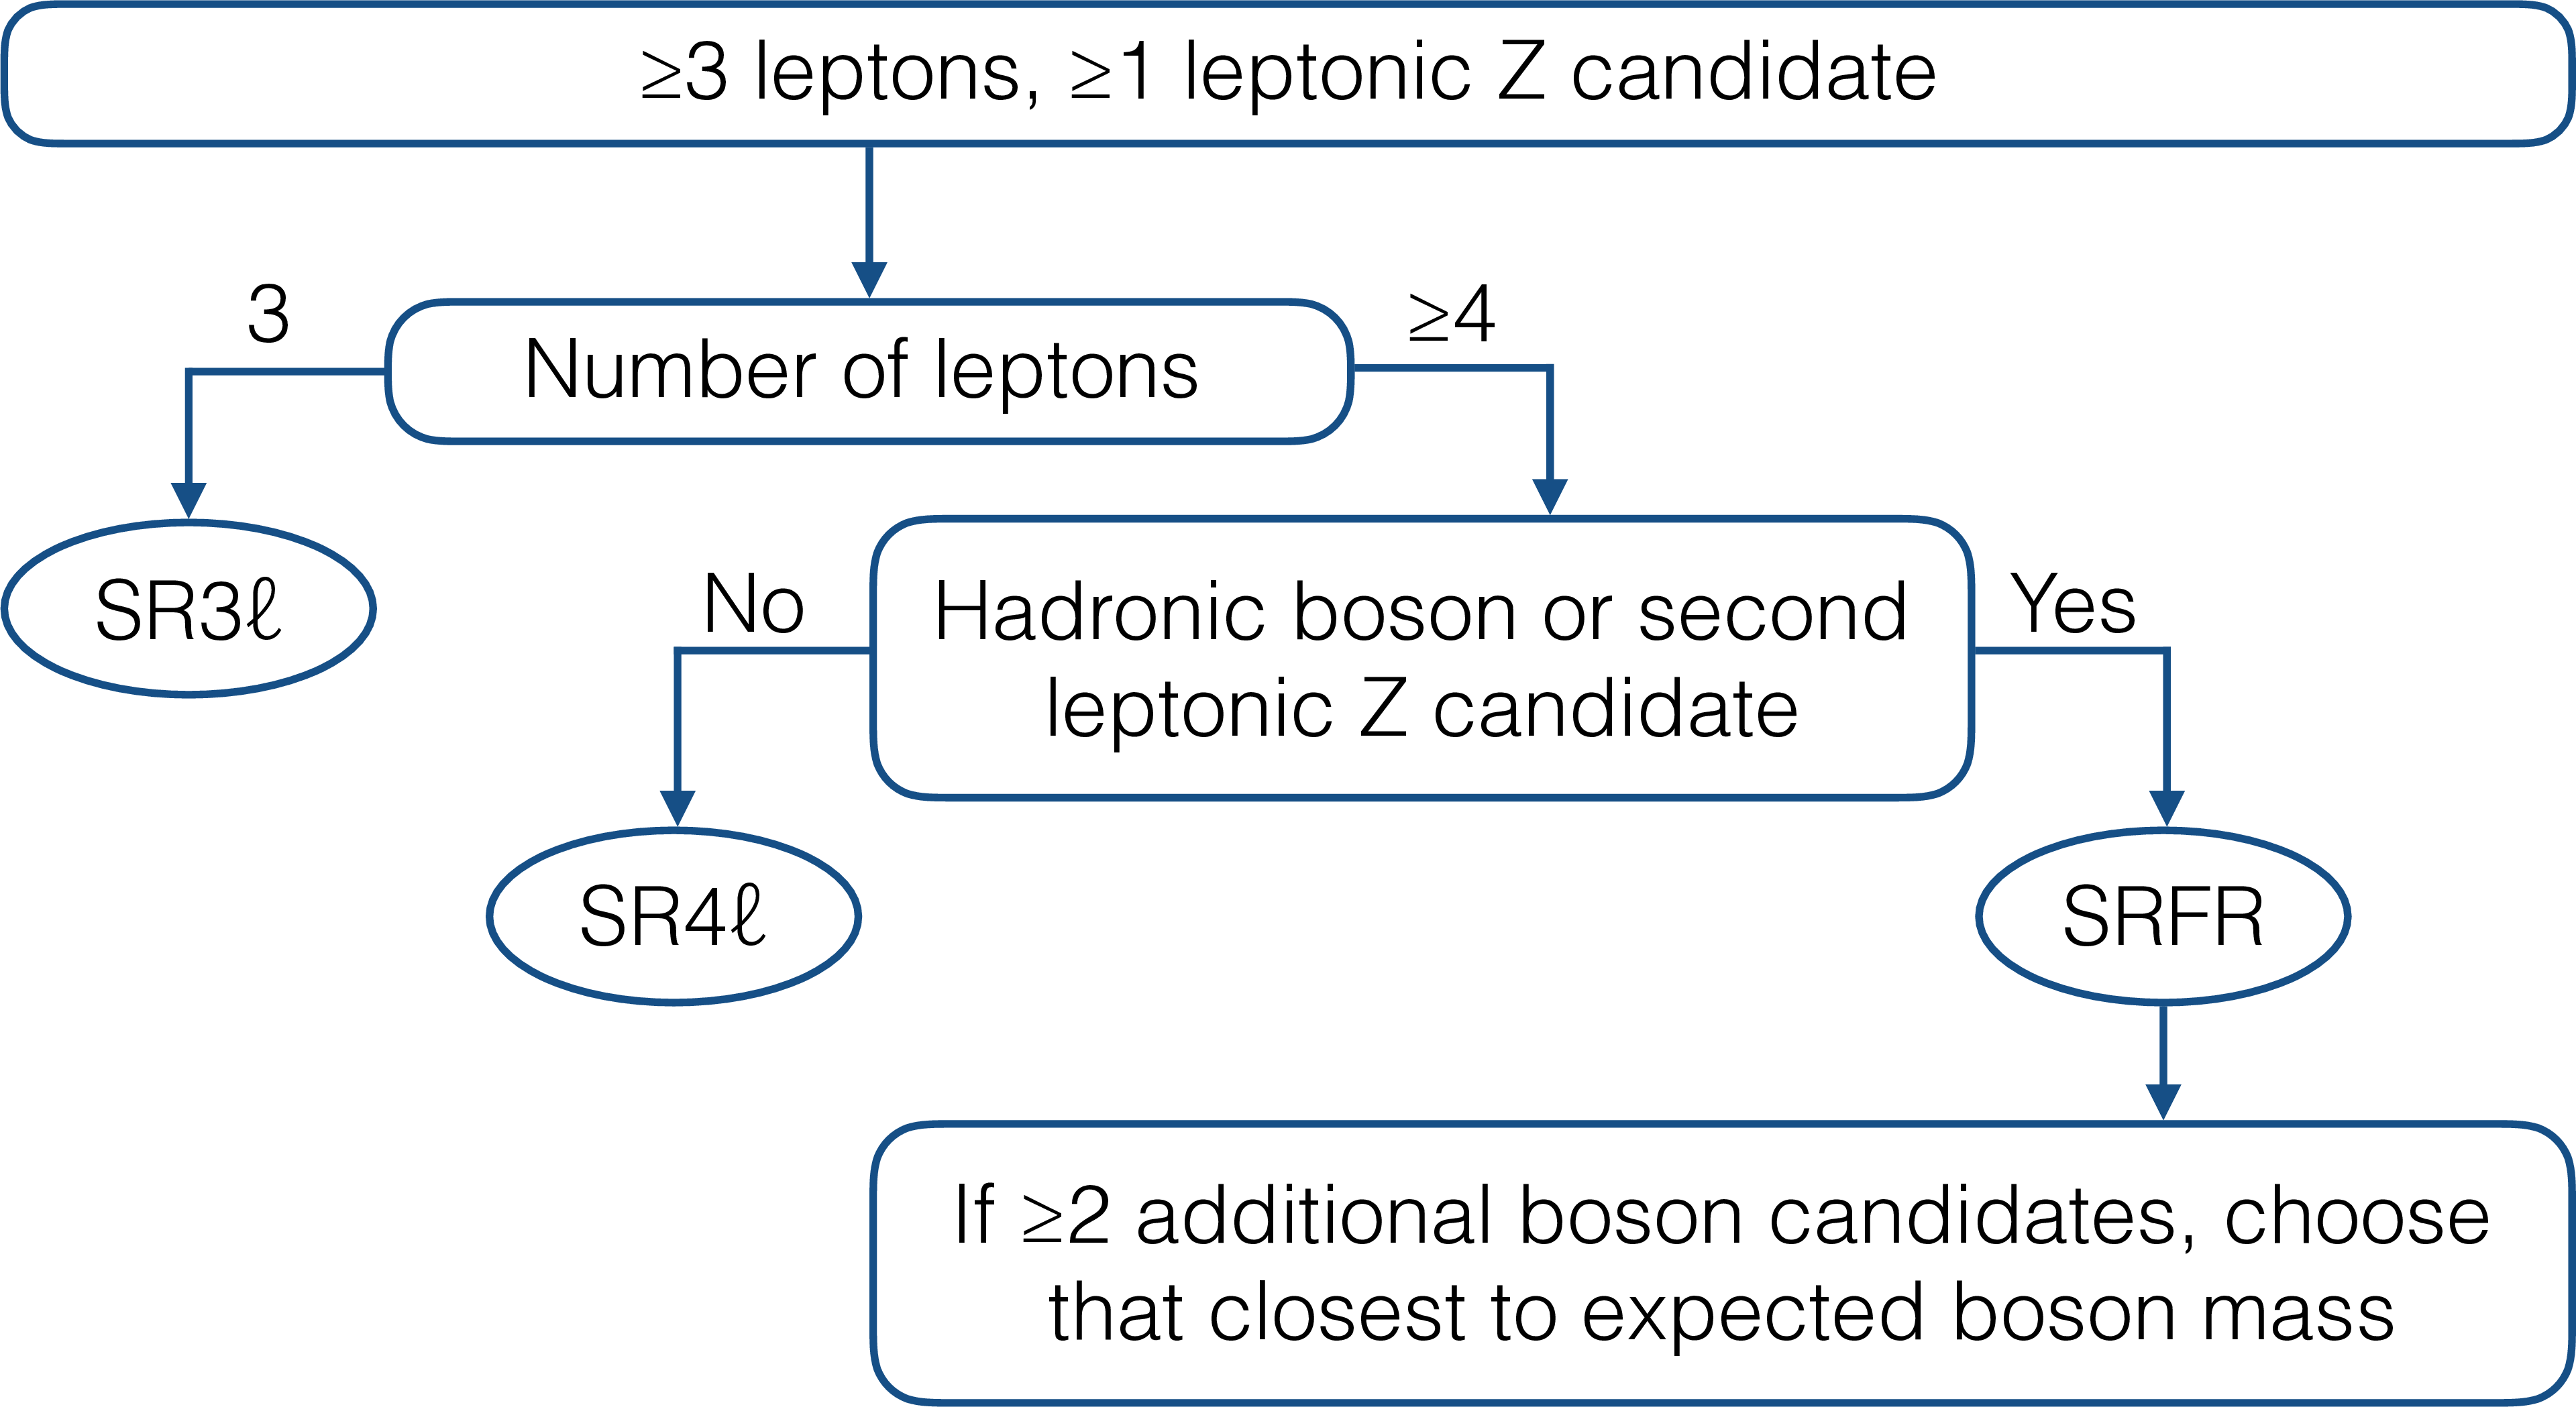
\includegraphics[width=0.98\textwidth]{figs/rpvthreel/3LRPVSchematic.png}
    %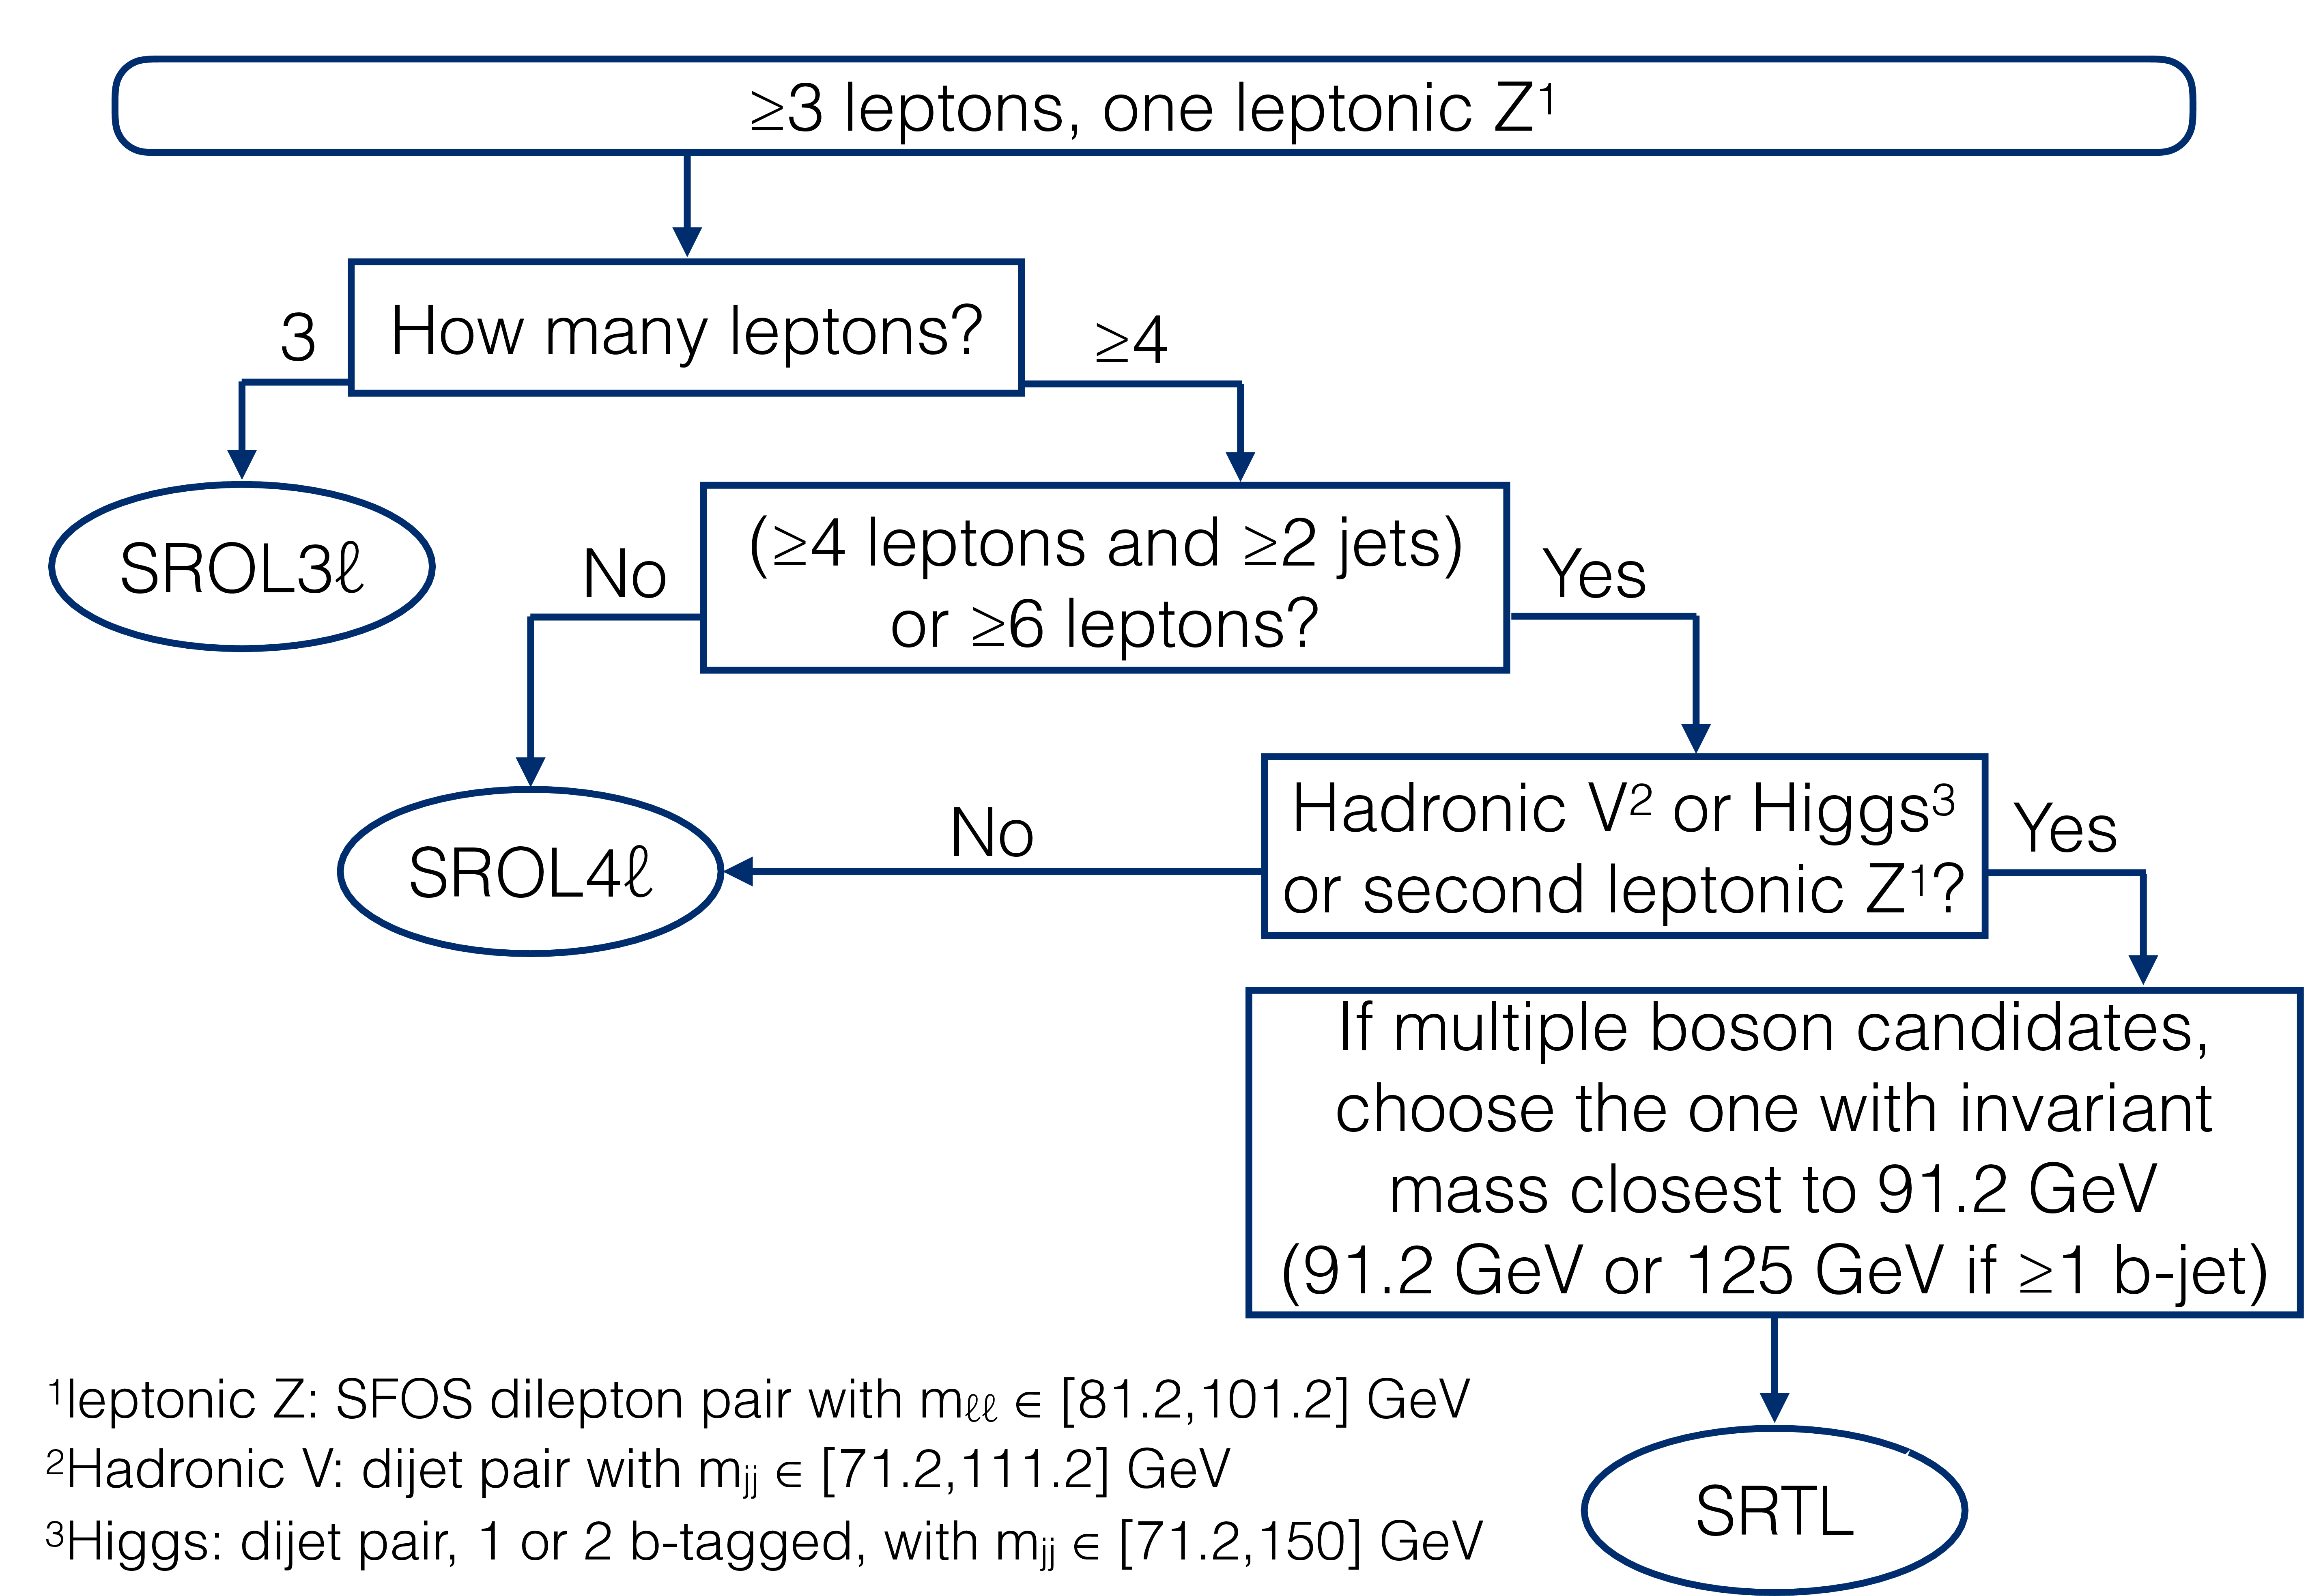
\includegraphics[width=0.98\textwidth]{figs/rpvthreel/regionCutflow.pdf}
  \end{center}
  \caption[Signal region flow chart]
          {Flow chart of selection algorithm dictating separation of events in the three main signal regions\cite{ATLAS:2020uer}}
          \label{fig:schematic}
\end{figure}

\subsubsection{\SRThree}
\label{sec:srthree}
The signal region requires exactly three light leptons, two of which form a SFOS pair within the \Zboson\ mass window of [81.2~\gev, 101.2~\gev].
If there are two SFOS sign candidates the candidate that is closest to the \Zboson\ mass is chosen.
The trilepton mass \mZl is then is then calculated.
Events in \SRThree are expected to exhibit a significant \met\ in final states where the other \chono decays has neutrinos in the final state, either directly for \chone$\rightarrow$\Wboson$\nu$ and \none$\rightarrow$\Hboson$\nu$ or \Zboson$\nu$, or from the subsequent decay of the \Wboson , \Zboson\ or Higgs boson.
A requirement of \met\ $>$ 150~\GeV reduces contamination from SM processes with no neutrinos, particularly \Zjet events that include a \fake lepton.
The SM \WZ process with fully leptonic decays is also a significant contributor to \SRThree, and contains a single neutrino from the \Wboson\ decay.
The measured \met\ is therefore representative of the \pt\ of the neutrino, and the transverse mass \mT of the \Wboson\ boson can be reconstructed from the \pt\ of the lepton and the azimuthal separation $\Delta\phi$ between the lepton and \pt$^{miss}$, with
\begin{equation}
m_{\text{T}}(\ell,\nu) = \sqrt{2p_{\mathrm{T}}^\ell E_{\mathrm{T}}^{\mathrm{miss}}[1-\cos(\phi_{\ell}-\phi_{\mathrm{miss}})]}
\label{eq:mT}
\end{equation}
The \mT of a \Wboson\ boson has a kinematic edge at the \Wboson\ boson mass, and signal events in \SRThree usually produce lepton--\met\ pairings with a larger \mT.
The minimum \mT of all lepton--\met\ pairings for which the other two leptons form a SFOS pair, defined as \mTmin, is required to be \mTmin\ $>$ 125~\GeV in \SRThree.
This definition allows \WZ events to be rejected even if the incorrect SFOS pair was selected for the \Zboson\ boson.
Finally a cut in the angular separation between the highest \pt\ $b\textrm{-jets}$, \dRbb$>$~1.5 is made to guarantee orthogonality to \ttZ regions.
This is discussed in greater detail in Section \ref{sec:crttz}.
The full definition of cuts for this region are shown in the region summary Table \ref{tab:regions:regionBreakdown}.

It is useful here to see how many events of a specific signal final state are accepted into the signal region when compared to the theoretically predicted number of events produced at the LHC for those processes.
Composed of products of selections applied at every level of the analysis for a given mass and final state this acceptance is computed via Equation \ref{eq:trilep:acc}.
\vspace{0.3cm}\\
\makebox[\textwidth]{\parbox{1.1\textwidth}{%
\begin{equation}\label{eq:trilep:acc}
  \begin{split}
    \mathcal{A}_{SR,i,{\tilde\chi^\pm_1\tilde\chi^\mp_1}}=
    \frac{n_{SR,i,{\tilde\chi^\pm_1\tilde\chi^\mp_1}}}{N_{{\tilde\chi^\pm_1\tilde\chi^\mp_1}} \times F_{{\tilde\chi^\pm_1\tilde\chi^\mp_1}}} \times \frac{\sigma_{{\tilde\chi^\pm_1\tilde\chi^\mp_1}}}{\sigma_{{\tilde\chi^\pm_1\tilde\chi^\mp_1}} + \sigma_{{\tilde\chi^\pm_1\tilde\chi^0_1}}}, \hspace{0.2cm}
    \mathcal{A}_{SR,i,{\tilde\chi^\pm_1\tilde\chi^0_1}}=
    \frac{n_{SR, i, {\tilde\chi^\pm_1\tilde\chi^0_1}}}{N_{{\tilde\chi^\pm_1\tilde\chi^0_1}} \times F_{{\tilde\chi^\pm_1\tilde\chi^0_1}}} 
    \times \frac{\sigma _{{\tilde\chi^\pm_1\tilde\chi^0_1}}}{\sigma_{{\tilde\chi^\pm_1\tilde\chi^\mp_1}} + \sigma_{{\tilde\chi^\pm_1\tilde\chi^0_1}}}
  \end{split}
\end{equation}
}}
%\vspace{0.5cm}
where the number of events selected in a signal region from a specific final state $i$ in \CCsignal production is indicated by lower-case $n_{SR,i,{\tilde\chi^\pm_1\tilde\chi^\mp_1}}$ and the \emph{total} number of events generated for \CCsignal production is indicated by $N_{{\tilde\chi^\pm_1\tilde\chi^\mp_1}}$ ($\mathcal{O}(10^4)$), which is corrected by the filter efficiency (inverted) factor $F_{{\tilde\chi^\pm_1\tilde\chi^\mp_1}}$ ($\mathcal{O}(10^{2})$) determined by the MC generator in order to scale up to what would have been generated sans filters.
The acceptance is then multiplied by the ratio of the \CCsignal production cross section to the sum of the \CCsignal and \CNsignal production cross sections in order to show the relative importance of different final states from each production process. 
The similar formula for \CNsignal production is also shown.  Finally, note that to find the number of events expected in a signal region from a specific final state, the corresponding acceptance factor can simply be multiplied by the total production cross section and the integrated luminosity.  

Figure \ref{fig:AccSR3l} shows the acceptances for each specific final state as a function of the \chono mass from 100~\gev to 1200~\gev in steps of 50~\gev.
Branching ratios to bosons are democratic as well as to each lepton flavor.
The very first row with the label ``All'' row in the Figure is the total acceptance from all final states from both production processes.
The acceptance for the three lepton signal region, \SRThree, is shown in Figure~\ref{fig:AccSR3l}.
Having already explained that the top row is the total acceptance, note that approximately the upper third of the figure shows the acceptance for final states from the \CNsignal production process, while approximately the lower two-thirds shows  the final states from the \CCsignal production process.
The largest acceptance for \SRThree can indeed be seen to be from the final states that would be expected to have only three leptons (\Zboson$\ell$ \Zboson$\nu$, \Zboson$\ell$ \Hboson $\nu$, \Zboson$\ell$ \Wboson$\nu$).
The color scale is normalized to the largest acceptance from any single final state, which is $1.8 \times 10^{-3}$ for the \CNsignal$\rightarrow$\Zboson e \Zboson $\nu$ and \CNsignal$\rightarrow$\Zboson $\mu$ \Zboson $\nu$ final states for a \chone mass of 1200\GeV.

These figures are uploaded to the HEPData website associated with our analysis, which will allow reinterpretations in terms of future models.
%\makebox[\textwidth]{\parbox{1.1\textwidth}{
\begin{figure}[tbp]
  \begin{center}
    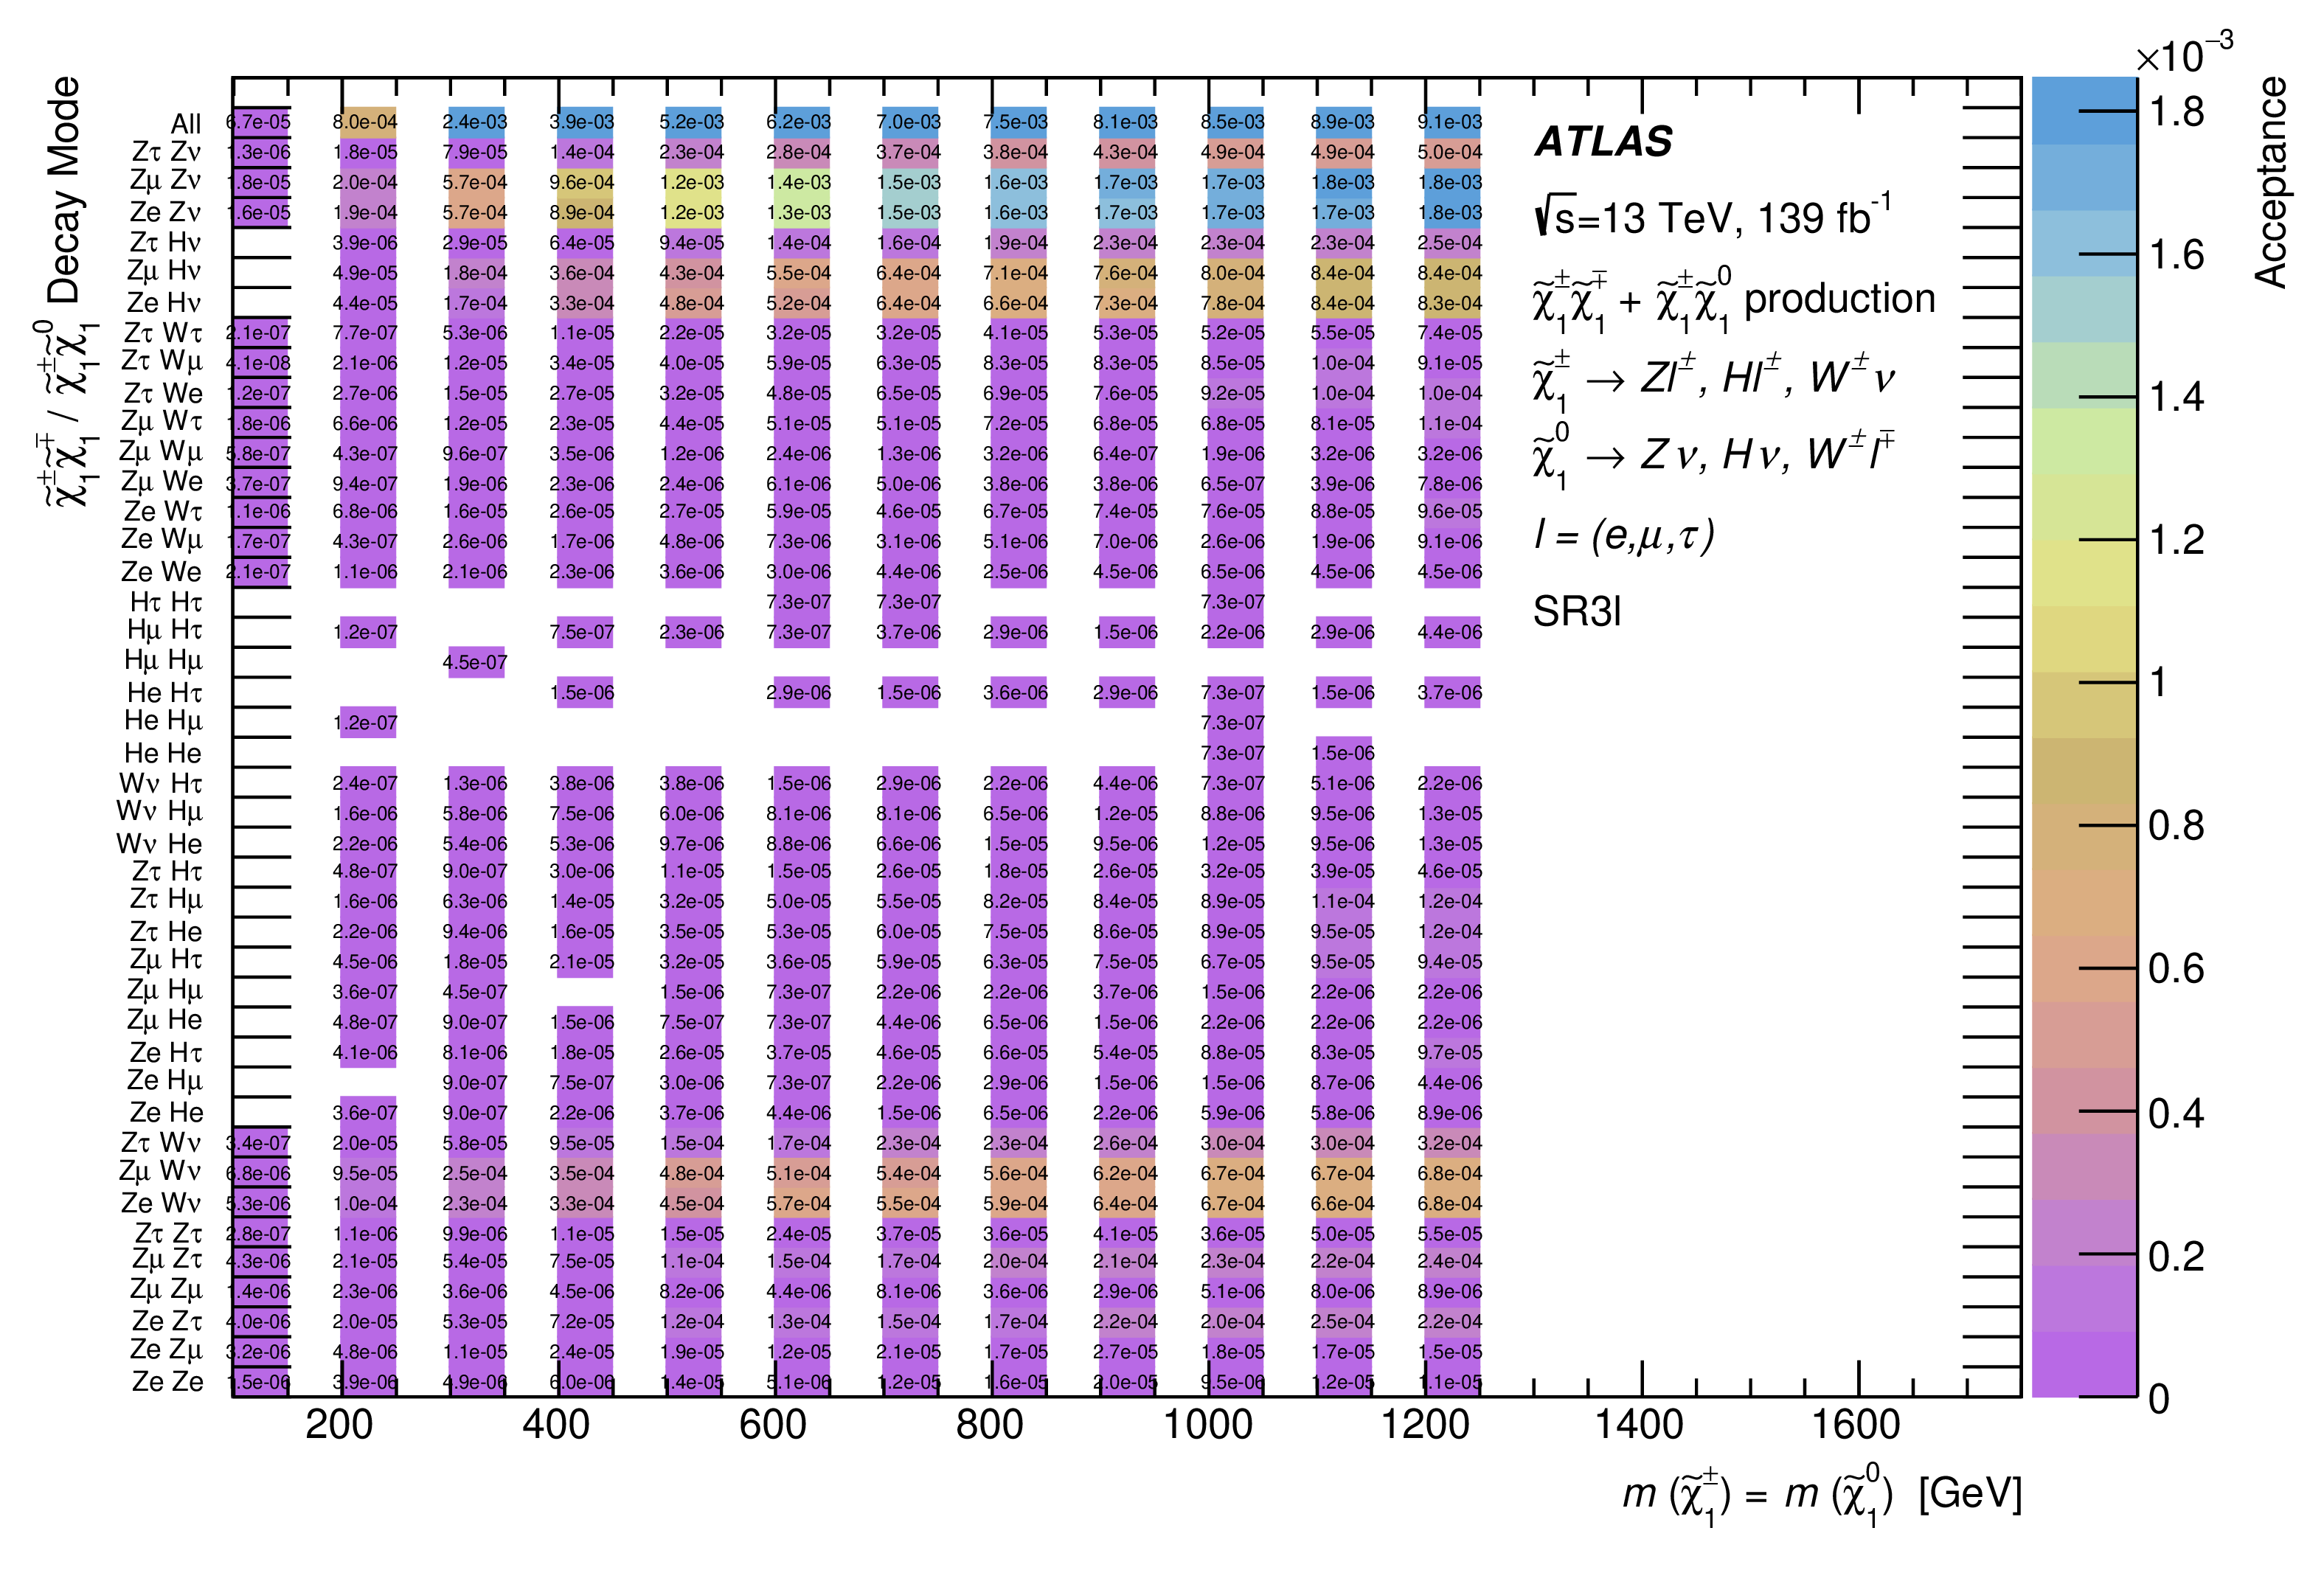
\includegraphics[width=0.98\textwidth]{figs/rpvthreel/MC_Acc_MassvsProcess_SROL3l_emutau.png}
  \end{center}
  \caption[Signal acceptance by process in \SRThree]
          {The truth-level acceptances for each decay mode of the generated \CCsignal + \CNsignal signals in the inclusive \SRThree region. Results are given as a function of \chono mass and the final state boson and lepton combination \cite{ATLAS:2020uer}.}
          \label{fig:AccSR3l}
\end{figure}

\subsubsection{\SRFR}
\label{sec:srfr}
To target fully visible events, \SRTL requires a fourth lepton and a second reconstructed \Zboson, \Wboson, or Higgs boson.
Pairs of jets are considered for the second boson if their invariant mass \mjj is consistent with that of a $W$ or $Z$ boson, with 71.2 $<$ \mjj\ $<$ 111.2~\GeV.
If at least one of the jets is a $b$-jet, the \mjj requirement is loosened to 71.2 $<$ \mjj\ $<$ 150~\GeV to allow for Higgs boson decays.
Additional SFOS lepton pairs are also considered for the second boson candidate in events with six or more leptons if their invariant mass is consistent with the $Z$ boson mass, such that 81.2 $<$ \mll $<$ 101.2~\GeV.
If there are multiple candidates for the second boson, the pairing selected is that with invariant mass closest to the \Zboson\ boson mass, or closest to the Higgs boson mass for pairs that include at least one $b$-jet.
The presence of one or more additional leptons from the second \chono decay introduces ambiguity in the assignment of a lepton and boson produced directly from a \chono decay.
So in order to form the correct invariant masses (\mZl, \mBl) a matching procedure is implemented to identify the leptons that come directly from the \chono decays, rather than from the subsequent decay of a boson, and to assign them to each \chono.
The procedure optimizes the sensitivity to signals of various masses by maintaining a high efficiency for the correct assignments while reducing the contamination from SM processes.
In \SRFR, both the trilepton decay and the fully visible decay of the second \chono, with reconstructed mass \mBl, are chosen as the groupings that minimize the mass asymmetry between the mass-degenerate \CCsignal or \CNsignal pair, where \mZlAsym is defined as
\begin{equation}
  m_{Z\ell}^{\mathrm{asym}}= \frac{|m_{Z\ell} - m_{\tilde\chi,2}|}{m_{Z\ell} + m_{\tilde\chi,2}}
  \label{eq:asym}
\end{equation}
Again a cut of \dRbb$>$~1.5 is made to guarantee orthogonality to \ttZ regions.
The acceptance for \SRFR is shown in Figure~\ref{fig:AccSRFR} and can be seen to be from the final states that are expected to have four or more leptons and two jets (\Zboson$\ell$ \Wboson$\ell$, \Zboson$\ell$ \Hboson$\ell$, \Zboson$\ell$ \Zboson$\ell$).
The color scale is normalized to the largest acceptance from any single final state, which is $0.29 \times 10^{-3}$ for the \CCsignal$\rightarrow$\Zboson$e$ \Zboson$\mu$ final state for a \chone mass of 400~\GeV.   
\begin{figure}[tbp]
  \begin{center}
    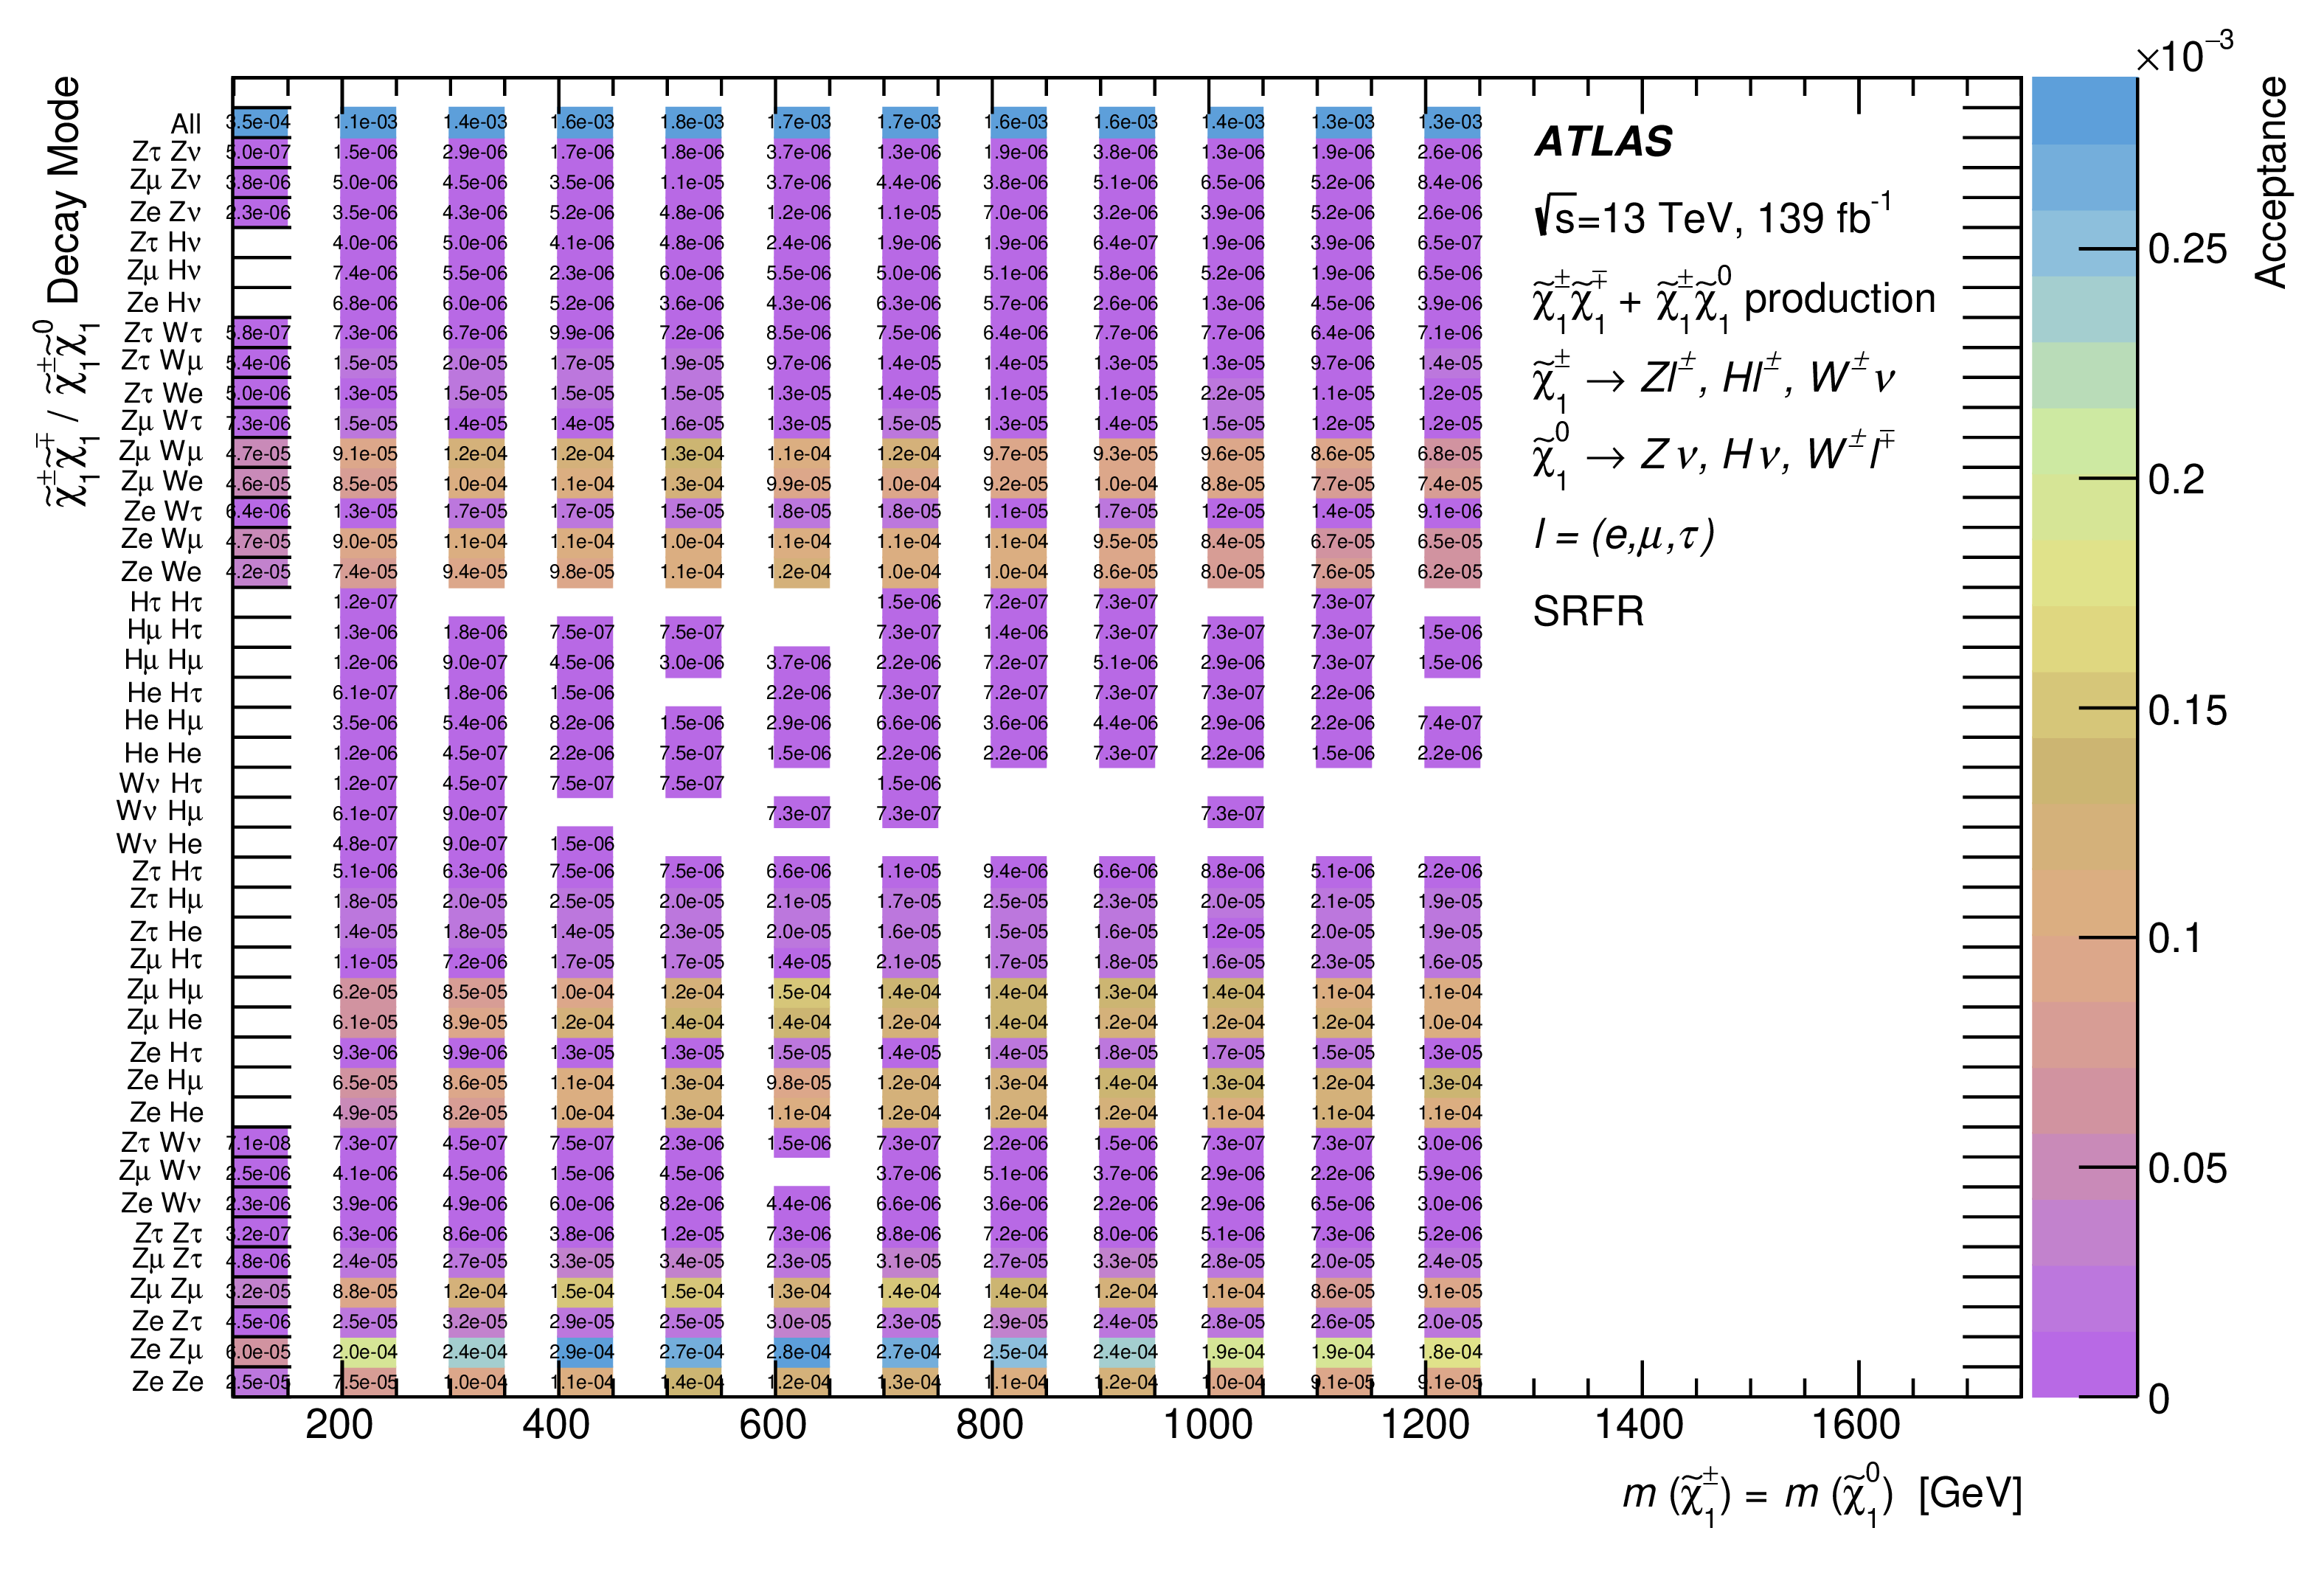
\includegraphics[width=0.98\textwidth]{figs/rpvthreel/MC_Acc_MassvsProcess_SRTL_emutau.png}
  \end{center}
  \caption[Signal acceptance by process in \SRFR]
          {The truth-level acceptances for each decay mode of the generated \CCsignal + \CNsignal signals in the inclusive \SRFR region. Results are given as a function of \chono mass and the final state boson and lepton combination~\cite{ATLAS:2020uer}.}
          \label{fig:AccSRFR}
\end{figure}

\subsubsection{\SRFour}
\label{sec:srfour}
The \SRFour region targets events in which the decay of the second \chono includes one or more leptons but cannot be fully reconstructed, for example due to the presence of neutrinos in the final state.
Events with four or more leptons that fail \SRTL requirements are are collected in \SRFour.
The optimal matching procedure to form the correct \mZl was found to be a combination of two separate methodologies that are chosen based on a threshold criterion value of \Lt, the scalar sum of the \pt\ of all the leptons in the event. 
Here \Lt acts as a proxy for the \chone mass.
In the low mass regime where \Lt\ $<$ 550~\GeV, the \chono can often be produced with a sufficiently large momentum such that the charged lepton and \Zboson\ boson are collimated, and \mZl is formed by choosing the lepton that is closest to the direction of the \Zboson\ boson candidate, i.e. the lepton with the smallest \dr to the \Zboson\ boson.
The second method targeting high-mass signals is used when \Lt\ $\geq$ 550~\GeV, the \chone decay products are often at a wide angle with respect to each other (back-to-back), and mispairings will produce a \mZl that is smaller than the \chone\ mass.
Therefore, the lepton that maximizes the reconstructed \mZl is chosen.
Again a cut of \dRbb$>$~1.5 is made to guarantee orthogonality to \ttZ regions.
The full definition of cuts for this region are shown in the region summary Table \ref{tab:regions:regionBreakdown}.
The process specific acceptance plot in Figure \ref{fig:AccSR4l} again shows good relative sensitivity to the the wide range of final states with neutrinos.
The color scale is normalized to the largest acceptance from any single final state, which is $0.42 \times 10^{-3}$ for the \CCsignal$\rightarrow$\Zboson$e$ \Zboson$\mu$ final state for a \chone mass of 1200~\GeV. 
\begin{figure}[tbp]
  \begin{center}
    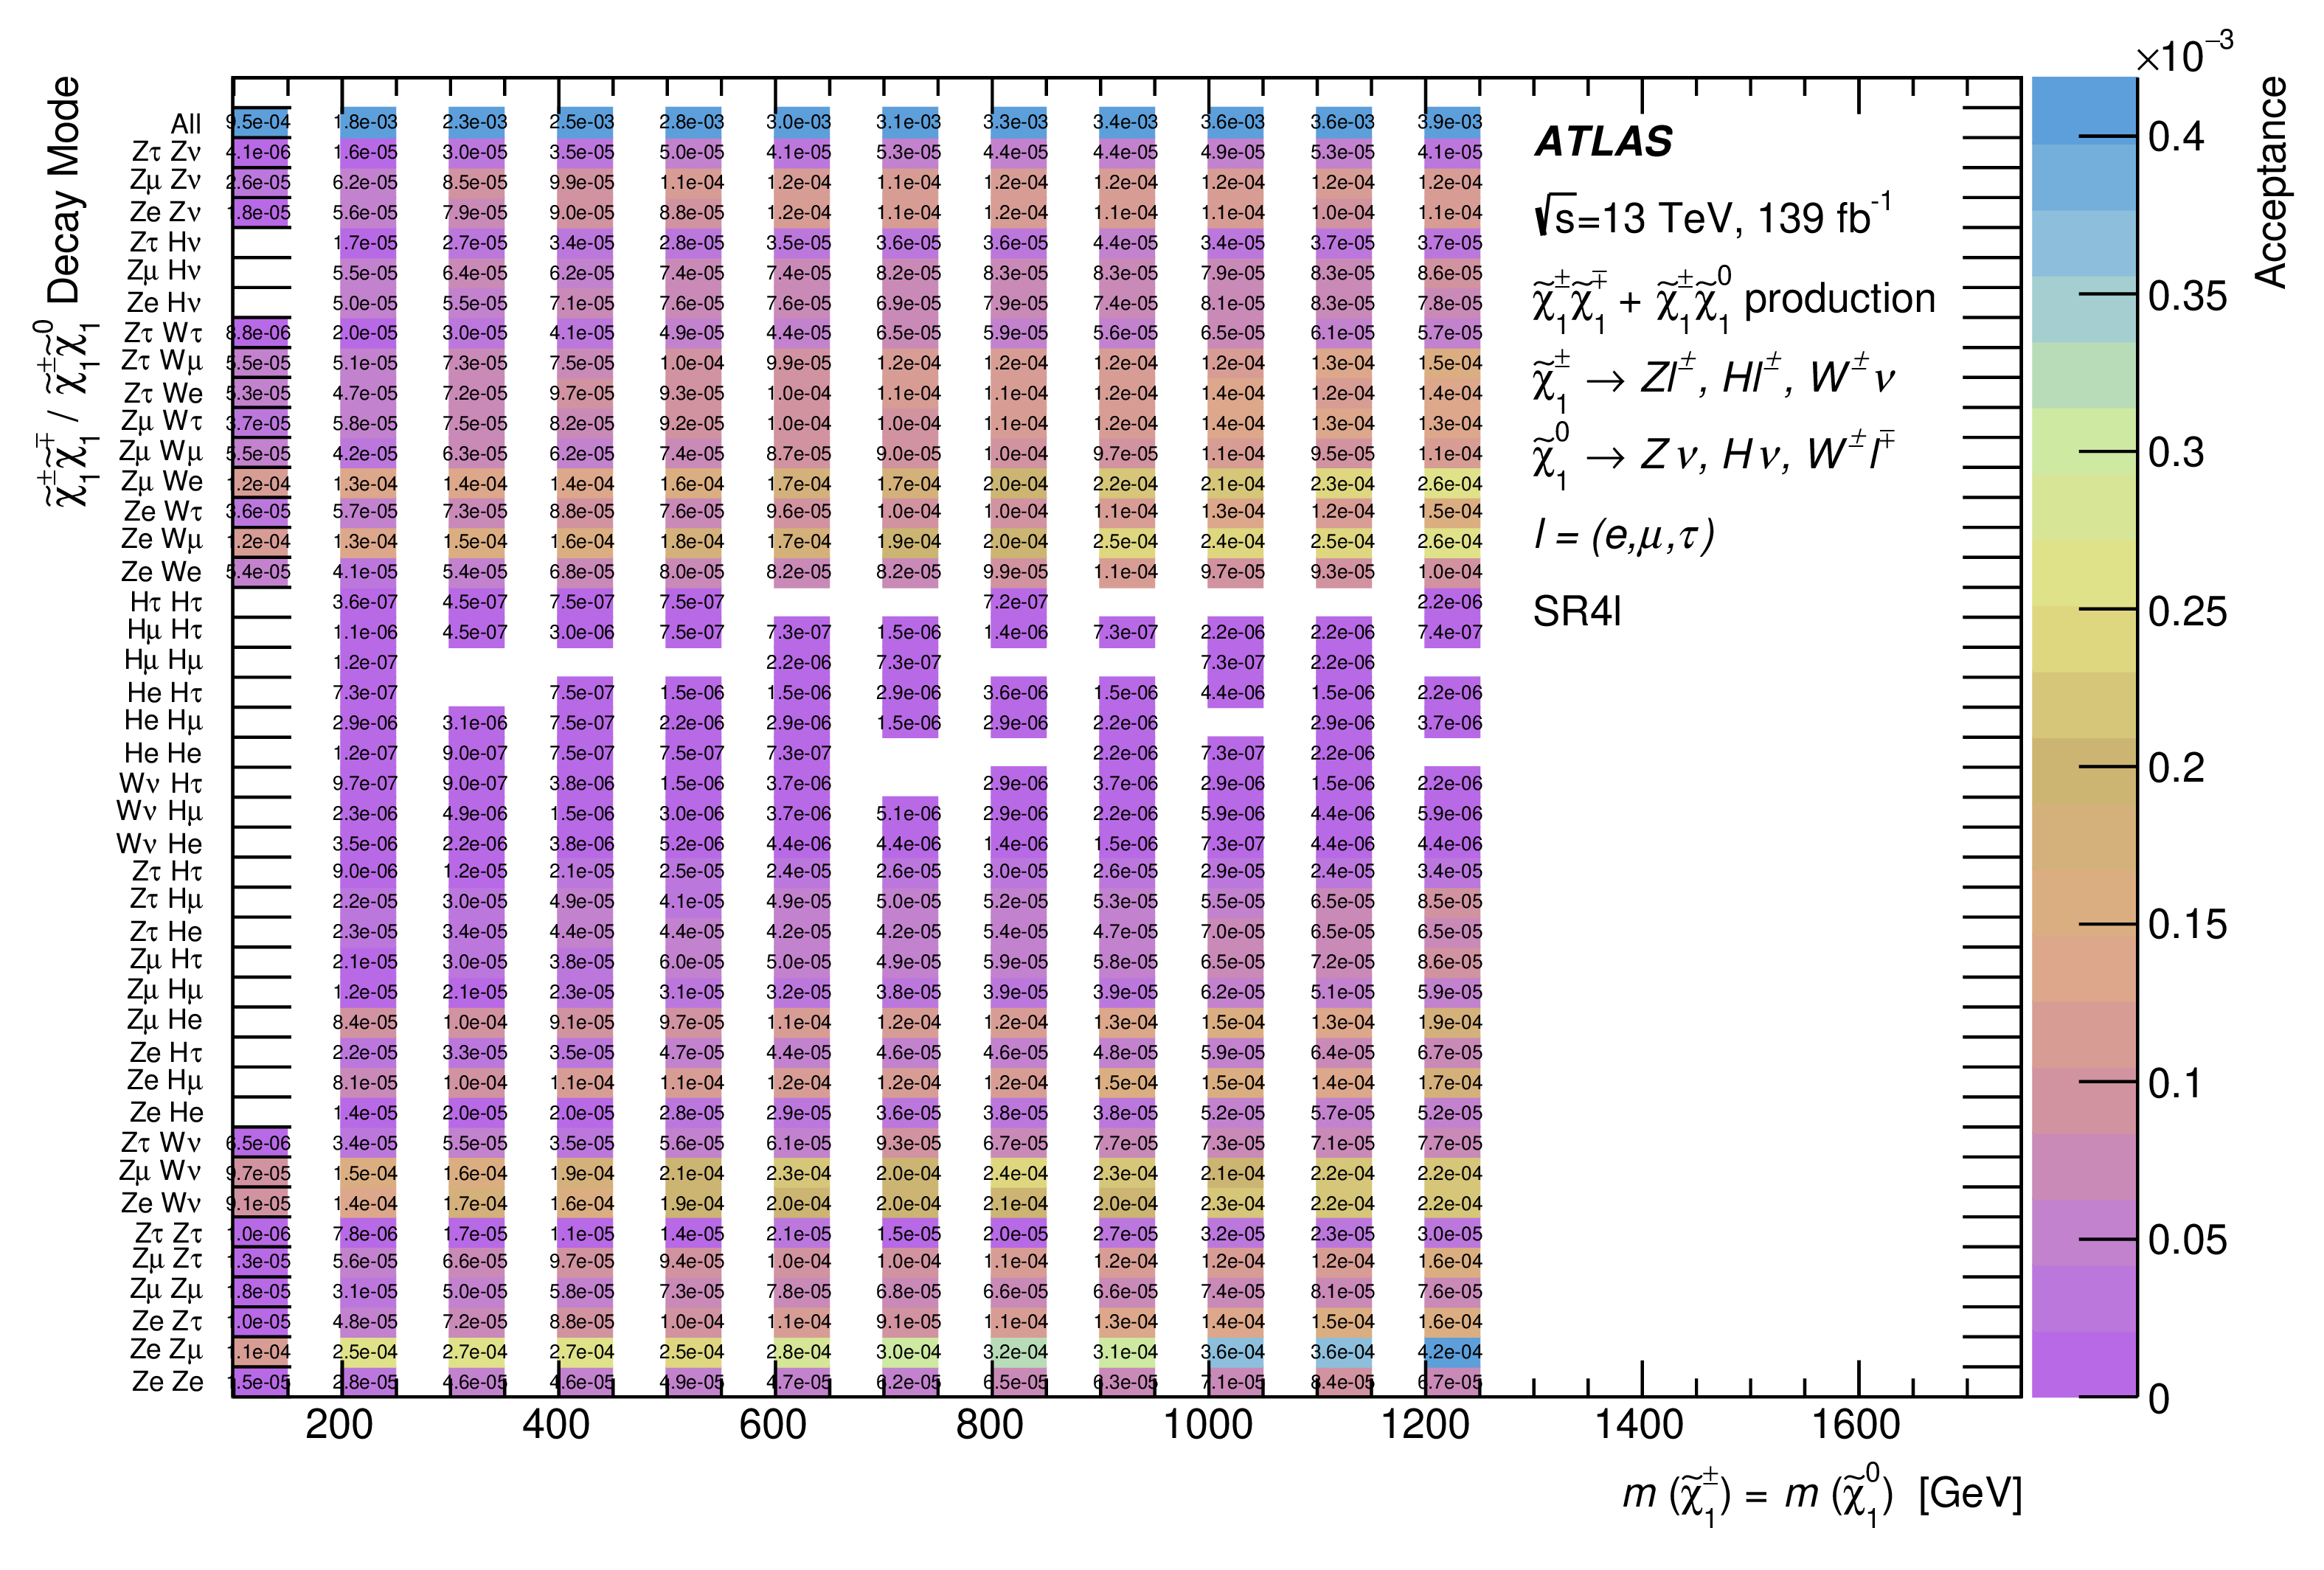
\includegraphics[width=0.98\textwidth]{figs/rpvthreel/MC_Acc_MassvsProcess_SROL4l_emutau.png}
  \end{center}
  \caption[Signal acceptance by process in \SRFour]
          {The truth-level acceptances for each decay mode of the generated \CCsignal + \CNsignal signals in the inclusive \SRFour region. Results are given as a function of \chono mass and the final state boson and lepton combination~\cite{ATLAS:2020uer}.}
          \label{fig:AccSR4l}
\end{figure}

%The \SRThree region targets decays of the second \chono that include no leptons, requiring exactly three leptons in the event.
%\subsection{Rejection of Combination SM Backgrounds}
%\label{sec:combback}
\begin{figure}[htb]
    \centering
    \begin{subfigure}[b]{0.49\textwidth}
      \centering
      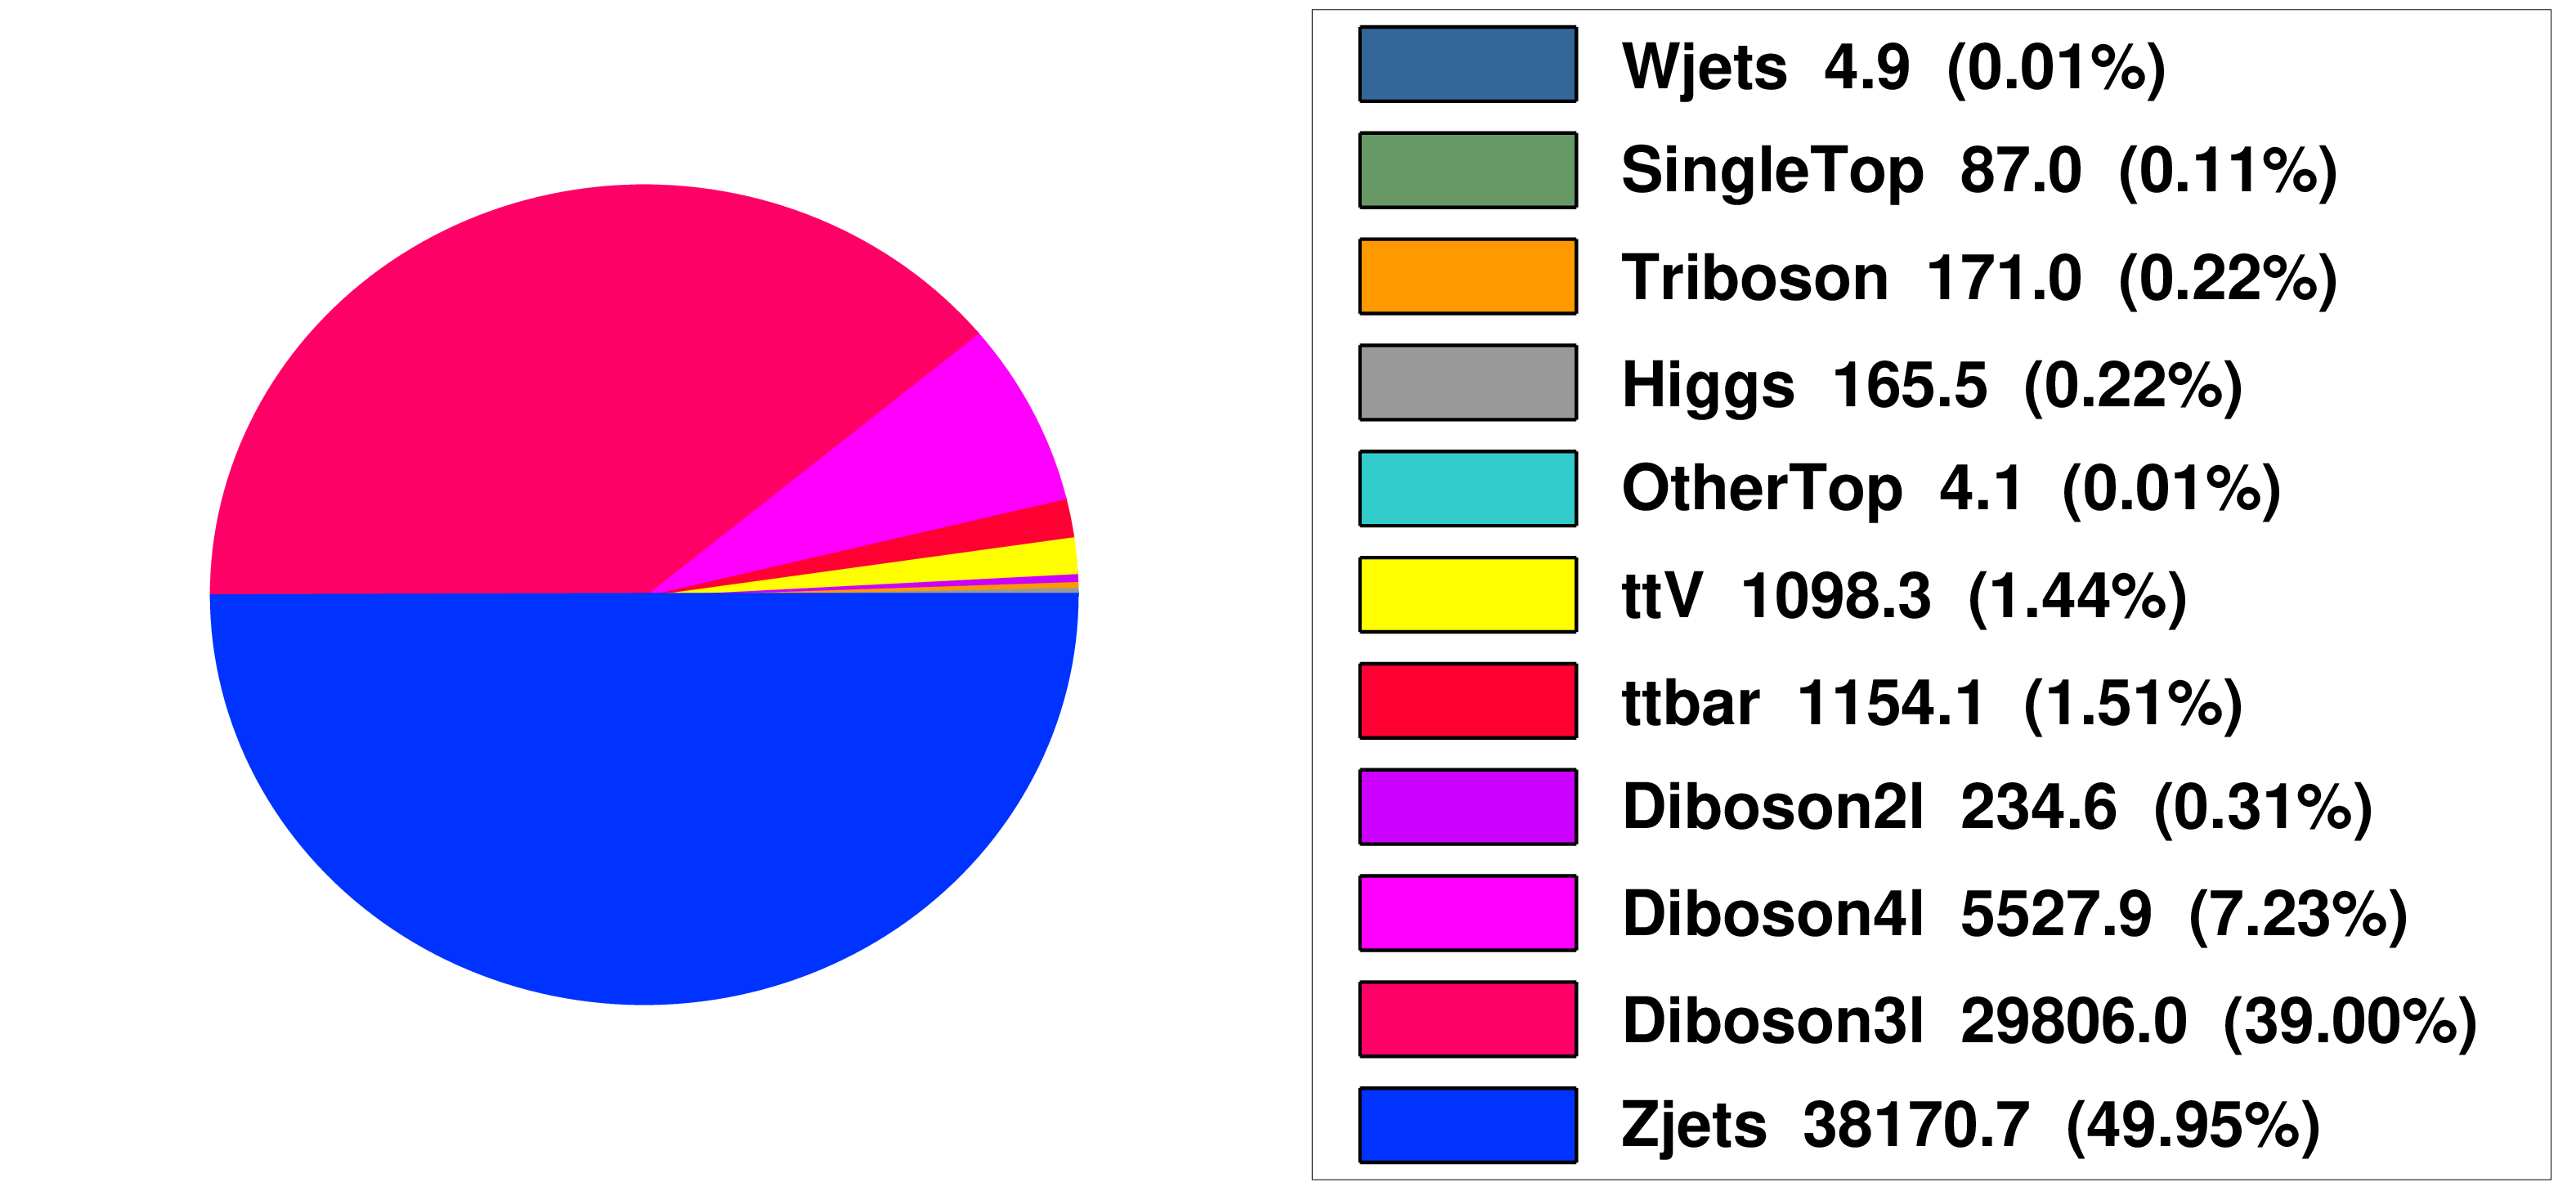
\includegraphics[width=0.98\textwidth]{figs/rpvthreel/bkgYields_SROL3l_noCuts.png}
      \caption{}
      \label{fig:pie_a}
    \end{subfigure}
    \hfill
    \begin{subfigure}[b]{0.49\textwidth}
      \centering
      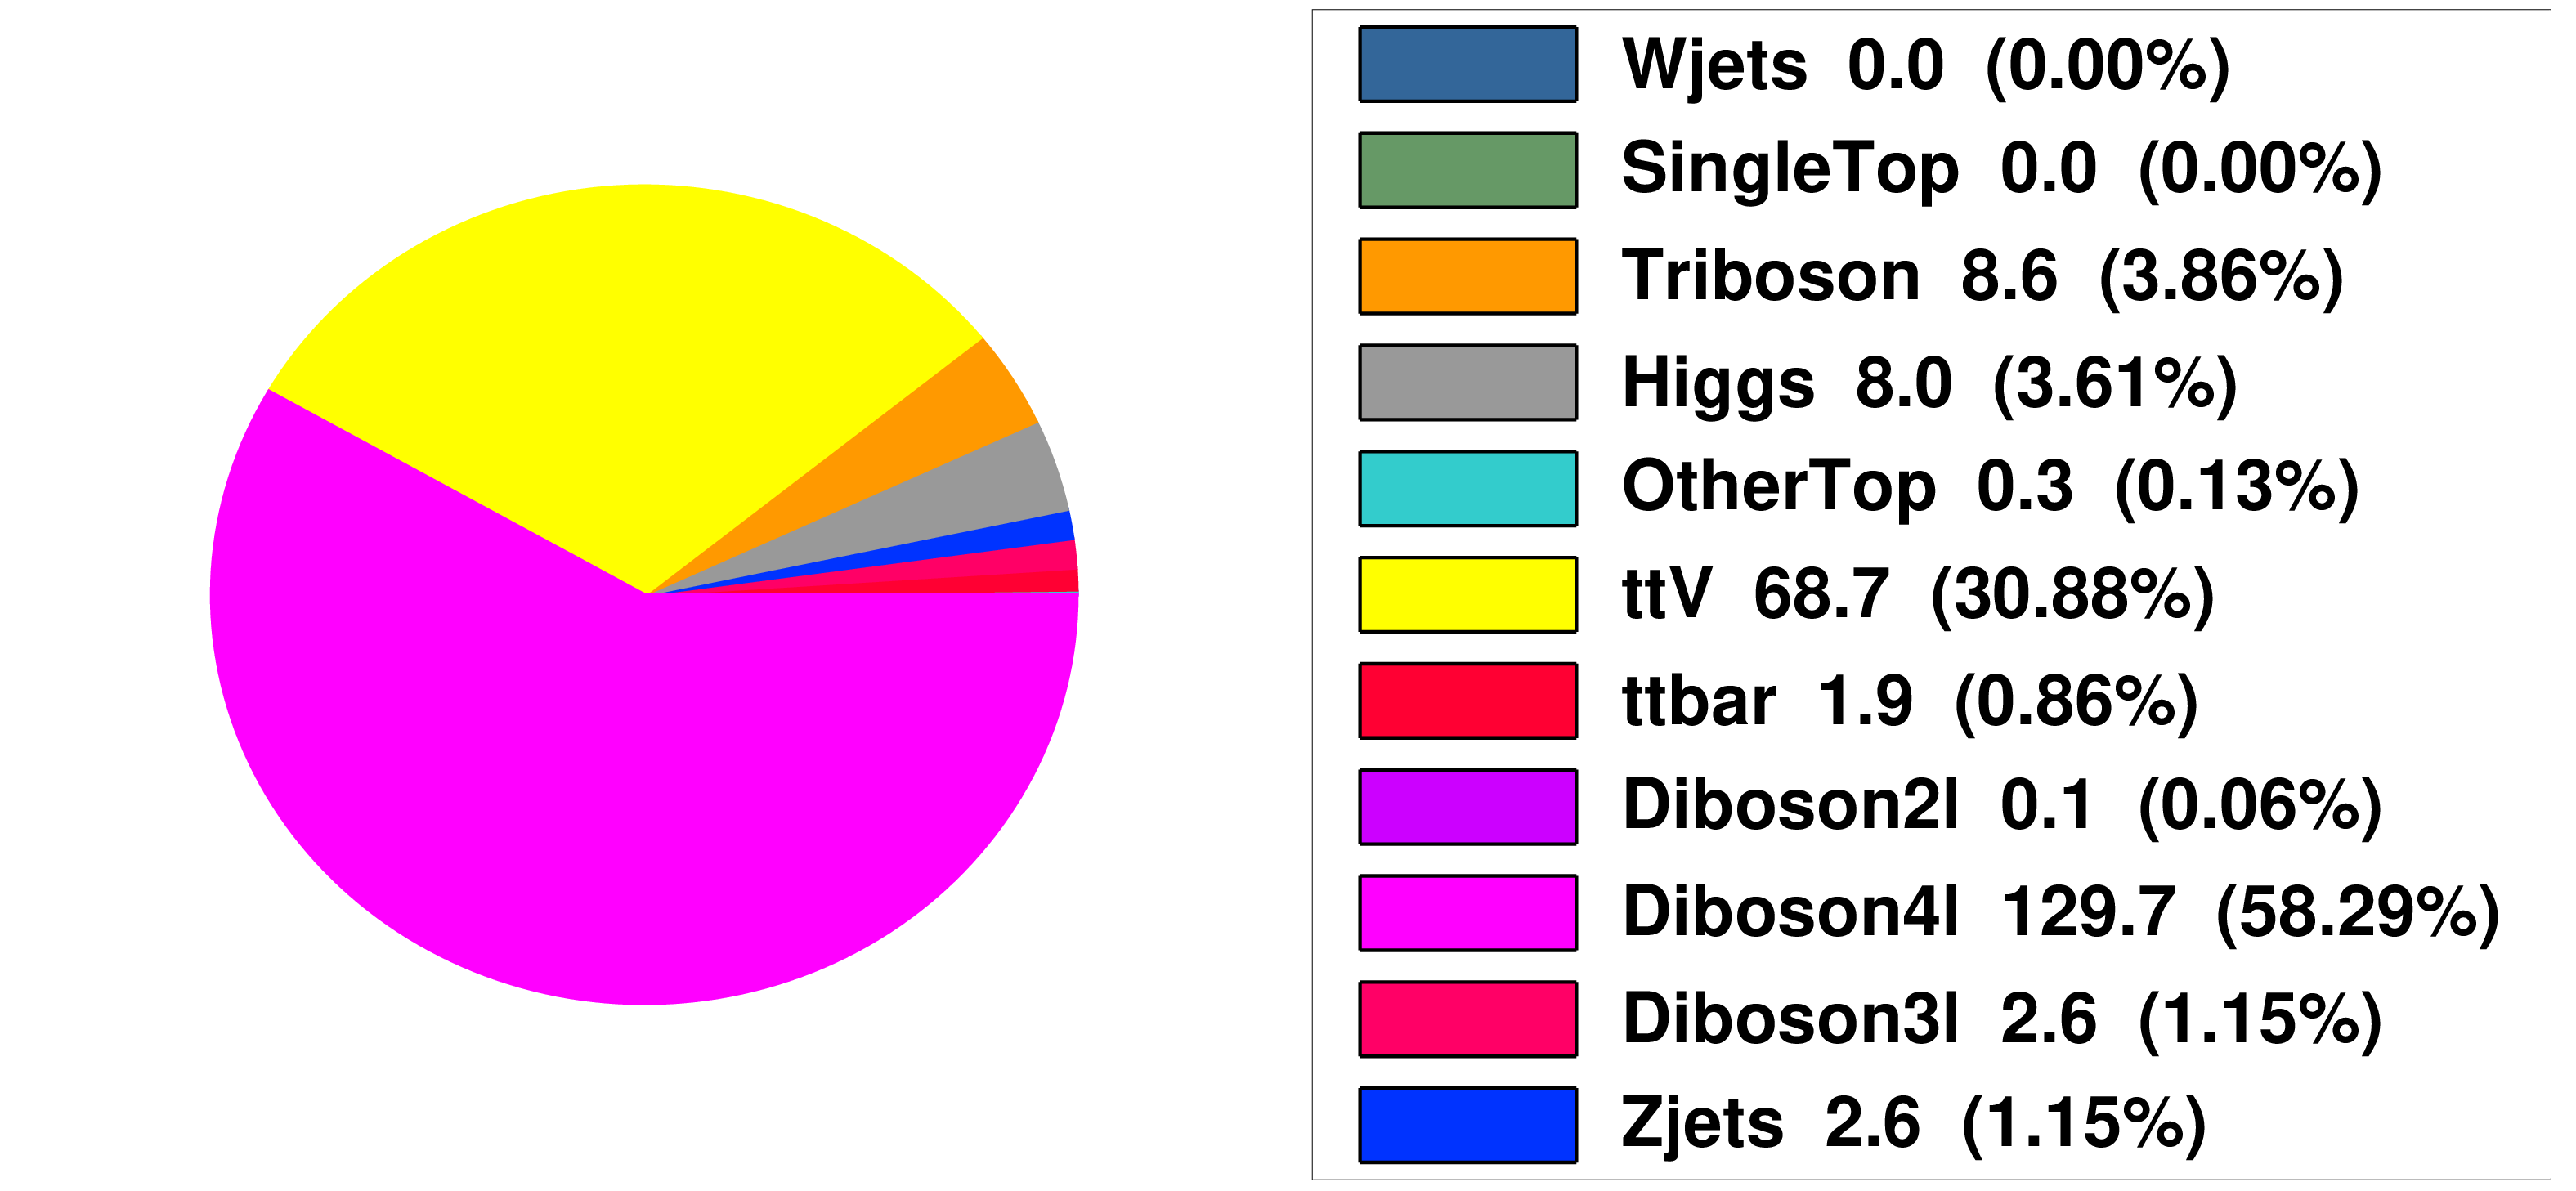
\includegraphics[width=0.98\textwidth]{figs/rpvthreel/bkgYields_SRTL_noCuts.png}
      \caption{}
      \label{fig:pie_b}
    \end{subfigure}
    \hfill
    \begin{subfigure}[b]{0.49\textwidth}
      \centering
      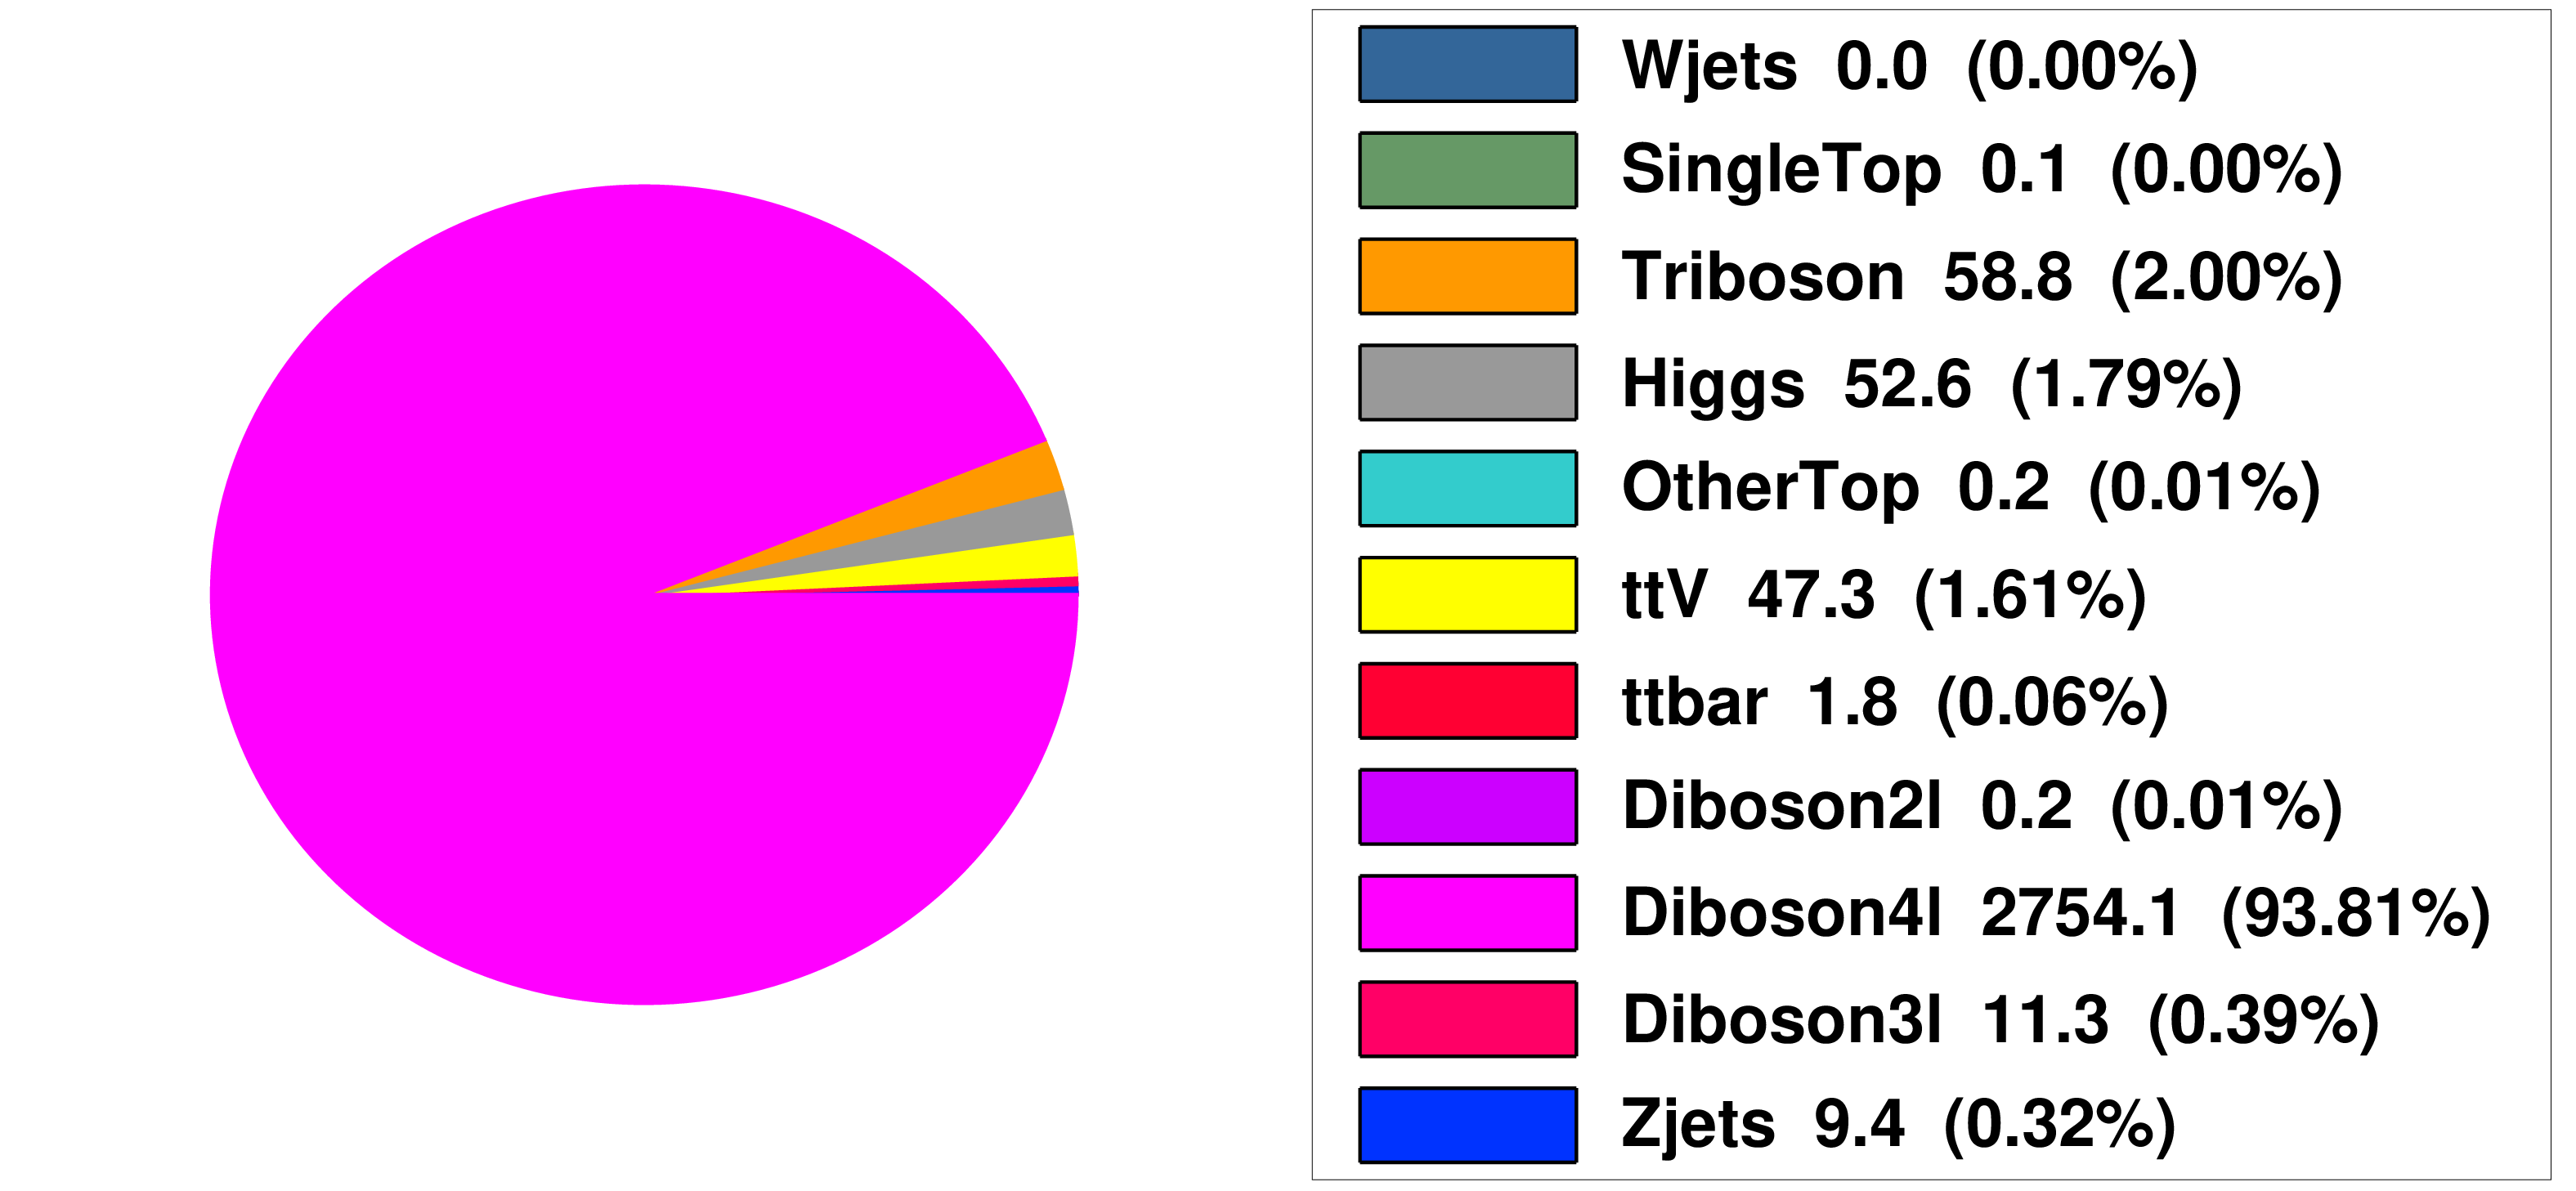
\includegraphics[width=0.98\textwidth]{figs/rpvthreel/bkgYields_SROL4l_noCuts.png}
      \caption{}
      \label{fig:pie_c}
    \end{subfigure}
    \caption{
    Expected yields from simulation for various background processes with (a) three leptons, four leptons (b) with and (c) without second boson candidate.
    Note that the kinematic requirements for the signal regions are not applied here.}
    \label{fig:PieYields}
\end{figure}

\subsection{Background Estimation and Validation}
As cursorily stated in Section \ref{sec:MC} the dominant backgrounds that contribute in the signal regions are \WZ, \ZZ, \ttZ, and \Zjets. 
Just how dominant is made clear from Figure~\ref{fig:PieYields}, which shows the relative background contributions estimate from simulation for events with three leptons, and for events with four leptons with and without a second boson candidate.
The additional region-specific kinematic requirements have not yet been applied here.
Note that in this figure, the many diboson processes are classified by the number of charged leptons in the final state.
Note that \WZ is the dominant diboson process with three leptons (classified as \small{\bf{Diboson3l}}), and \ZZ is the dominant diboson process with four leptons (classified as \small{\bf{Diboson4l}}). 
So in order to be confident in our ultimate background estimation it becomes pertinent to employ more robust techniques beyond simply taking yields directly from MC for these major players.
The \WZ, \ZZ, and \ttZ  have \Zboson\ bosons with leptonic decays and additional leptons, these are treated the same methodologically by way of dedicated orthogonal control and validation regions which are high in purity of the relevant background. 
The remaining large background, \Zjets, however is largely contributing by the misidentification of a jet as a lepton and is handled by a data-driven ``fake factor" method.
%are subjected to further 
%For the \SRThree region this ends up being \Zjets and \WZ (Diboson3l).
%One can see from Figure \ref{}, what \WZ amounts to about a third of total background while \Zjets contributes nearly half before any cuts are applied.
%For \SRFour the main contributor is coming from \ZZ (Diboson4l), accounting for nearly 94\% of the background share in that region (Figure \ref{}).
%For \SRFR we again see a large \ZZ contribution as well as a sizeable amount of \ttZ (ttV). 
\subsubsection{Handling Backgrounds: \emph{fake} Leptons }
\label{sec:fakes}
As it is required for all regions, the background estimate from fake-leptons will be described first.
In this analysis \emph{fake}-leptons or ``\emph{fakes}" are defined as misidentified prompt (light) leptons.
Or in other words any event object that is identified as prompt light lepton that is \emph{not} a prompt light lepton, is a \emph{fake}.
It is therefore important to determine the rate at which this misidentification occurs in all relevant kinematic regions. 
The most relevant sources for this analysis include the in-flight decays of heavy-flavor hadrons (HF) and misidentified light-flavor jets or in-flight decays of pions and kaons (LF).
The pair production of two electrons from the conversion of a prompt photon (Conv) is also considered a \emph{fake}-lepton process but makes a minor contribution.
In this analysis the relevant \emph{fake} processes (and their sources) are \Zjets (LF, HF) and \ttbar (HF) in the three-lepton regions and \WZ (LF) and \ZZ (LF, Conv) in the four-lepton regions, with \SRTL also having a large contribution from \ttZ (HF).
Due to the difficult MC modeling made by the many sources of fake-lepton processes, each of which is kinematically different and provides a relative contribution to the background estimate that is dependent on the analysis phase-space, the approach that is used for estimating this background is a data-driven fake-factor method.
%\hspace*{\fill}$\S$~\bf{Measuring \emph{fake} Factors}\\

To measure the \emph{fake} factors, a region enriched in \Zjets type fake events is defined, \CRZj.
The \CRZj region sets itself apart from other to-be-defined regions in that it is not directly included in the fit, but is used to derive the \fake-lepton estimation in each analysis region.
Events in this region are selected by requiring two signal leptons that form an SFOS pair and with an invariant mass within 10~\GeV of the \Zboson\ boson mass.
One of the two signal leptons is required to have fired a single-lepton trigger, thus ensuring no selection bias from \fake leptons.
To enhance the \Zjets purity and reduce prompt-lepton event contamination from the \WZ process, \CRZj requires \met\ $<$ 30~\GeV and \mT\ $<$ 30~\GeV.
A third, unpaired baseline lepton is also required in the event and is designated as the \fake candidate.
A requirement on the trilepton invariant mass of \mThreel $>$ 105~\GeV reduces contamination from the $Z\rightarrow4\ell$ process.
This region is further split into so called nom-ID and anti-ID events.
Where nom-ID refers to events in which the \fake candidate passes all nominal lepton ID criteria, and anti-ID refers to events where the \fake candidate passes all but at least one of three criteria: lepton ID requirements, isolation, or the impact parameter criteria. 
The expected contamination by prompt-lepton events from \WZ and \ZZ processes, as estimated from MC simulation, is subtracted from both populations so that they better represent the yields from \fake-lepton sources.
From these two types of events we can define our \fake factors by Equation \ref{eq:fakefactors}. 
\begin{equation}
  F(i) = \frac{N_\text{ID, data}(i) - N_\text{ID, prompt MC}(i)}{N_\text{antiID, data}(i) - N_\text{antiID, prompt MC}(i)}
  \label{eq:fakefactors}
\end{equation}
Where the fake factor is parameterized as a function of specific kinematic quantity $i$.
Several parameterizations were studied and the one best suited to this phase space was determined to be the variable \pTcone, which is defined as the scalar sum of the lepton \pt\ and the track isolation \ptiso, that is the scalar sum of the \pt\ of all the tracks in the given lepton's isolation cone.
In general, \pTcone provides a better handle on the momentum of the underlying jet giving rise to the fake/non-prompt lepton.
Three \ptiso working points are employed depending of flavor and lepton \pt~ as seen in Equation \ref{eq:pTcone}.
\begin{equation}
  p_{\text{T}}^{\text{cone}} =
  \begin{cases}
    p_{\text{T}} + \text{ptvarcone20\_TightTTVA\_pt1000}, & \text{electron } \\
    p_{\text{T}} + \text{ptvarcone30\_TightTTVA\_pt1000}, & \text{muon w/ } p_{\text{T}} < 50 \text{ GeV} \\
    p_{\text{T}} + \text{ptcone20\_TightTTVA\_pt1000}, & \text{muon w/ } p_{\text{T}} > 50 \text{ GeV} \\
  \end{cases}
  \label{eq:pTcone}
\end{equation}
%\hspace*{\fill}$\S$~\bf{Applying \emph{fake} Factors}\\
Applying the \fake factors then involves defining an additional \emph{anti-ID} region for each analysis region where the \fake factors are to be applied.
This region meets the exact conditions of its corresponding region with the exception that at least one signal lepton is replaced with an anti-ID lepton.
The \fake factor can then be applied to the anti-ID region to determine the \fake estimate for the nominal region. 
%\hspace*{\fill}$\S$~\bf{Validating \emph{fake} Factors}\\
The validation of the \fake factors takes place in the orthogonal region of \VRZj, an intermediate \met~ region designed as to move closer to the other analysis regions while maintaining \Zjets purity.
%The \fake factors were well validated as can be seen in the aux. Figures \ref{}.
The full region definition is given in the summary Table \ref{tab:regions:regionBreakdown}.

\subsubsection{Handling Backgrounds: \WZ}
\label{sec:crwz}
With the \WZ process being the dominant background in the three lepton region, dedicated control and validation regions are designed to constrain its normalization, a method described later in Section~\ref{sec:stats}.
Natural discrimination for this background with a \Wboson$\rightarrow\ell\nu$ decay is provided by the missing transverse energy from the neutrino and a kinematic variable that targets the \Wboson\ boson mass.
For this we look to \mTmin (Equation~\ref{eq:mTmin}), which inherits from the standard definition of \mT in Equation \ref{eq:mT},
%This distribution will have a kinematic edge at the \Wboson\ mass for the  \Wboson\ $\rightarrow \ell \nu$ channel. 
defined as the minimization of \mT when considering all leptons in the event while still always being able to form a SFOS pair. 
\begin{equation}
m_{\mathrm{T}}^{\mathrm{min}} = min(m_{\mathrm{T}}(\ell_{i},\nu))),~~ i=1,2,3
\label{eq:mTmin}
\end{equation}
Where $i$ indexes the three leptons.
The \mTmin is chosen over the standard \mT as the main discriminator in the \WZ regions because while the \Zboson\ reconstruction efficiency is high ($>$95\%) for signal, the SM \WZ background can have an off-shell \Zboson\ and a selection which matches leptons to form a mass closest to the nominal \Zboson\ pole mass may not choose the correct leptons from an off-shell \Zboson. 
It was found that for signal \mT and \mTmin are often the same quantity as expected from the high reconstruction efficiency, but for background it is found that \mTmin is often much lower than \mT and is more consistent with the kinematic edge at the \Wboson\ mass. 
Again a cut of \dRbb$>$~1.5 is made to guarantee orthogonality to \ttZ regions.
The full definition of cuts for the control region for \WZ and two associated validation regions that check extrapolation in mtmin and missing et are shown in the region summary Table~\ref{tab:regions:regionBreakdown} and illustrated in Figure~\ref{fig:3lorthogonality}.
The expected yields in the control and validation regions for \WZ are shown in Figure~\ref{fig:CRVRWZ_yields}.
The \mTmin and \met\ distributions are shown in Figure~\ref{fig:dataMCagreement_CRVR}, where good agreement is seen between data and the post-fit background estimates.
\begin{figure}[tbp]
  \begin{center}
    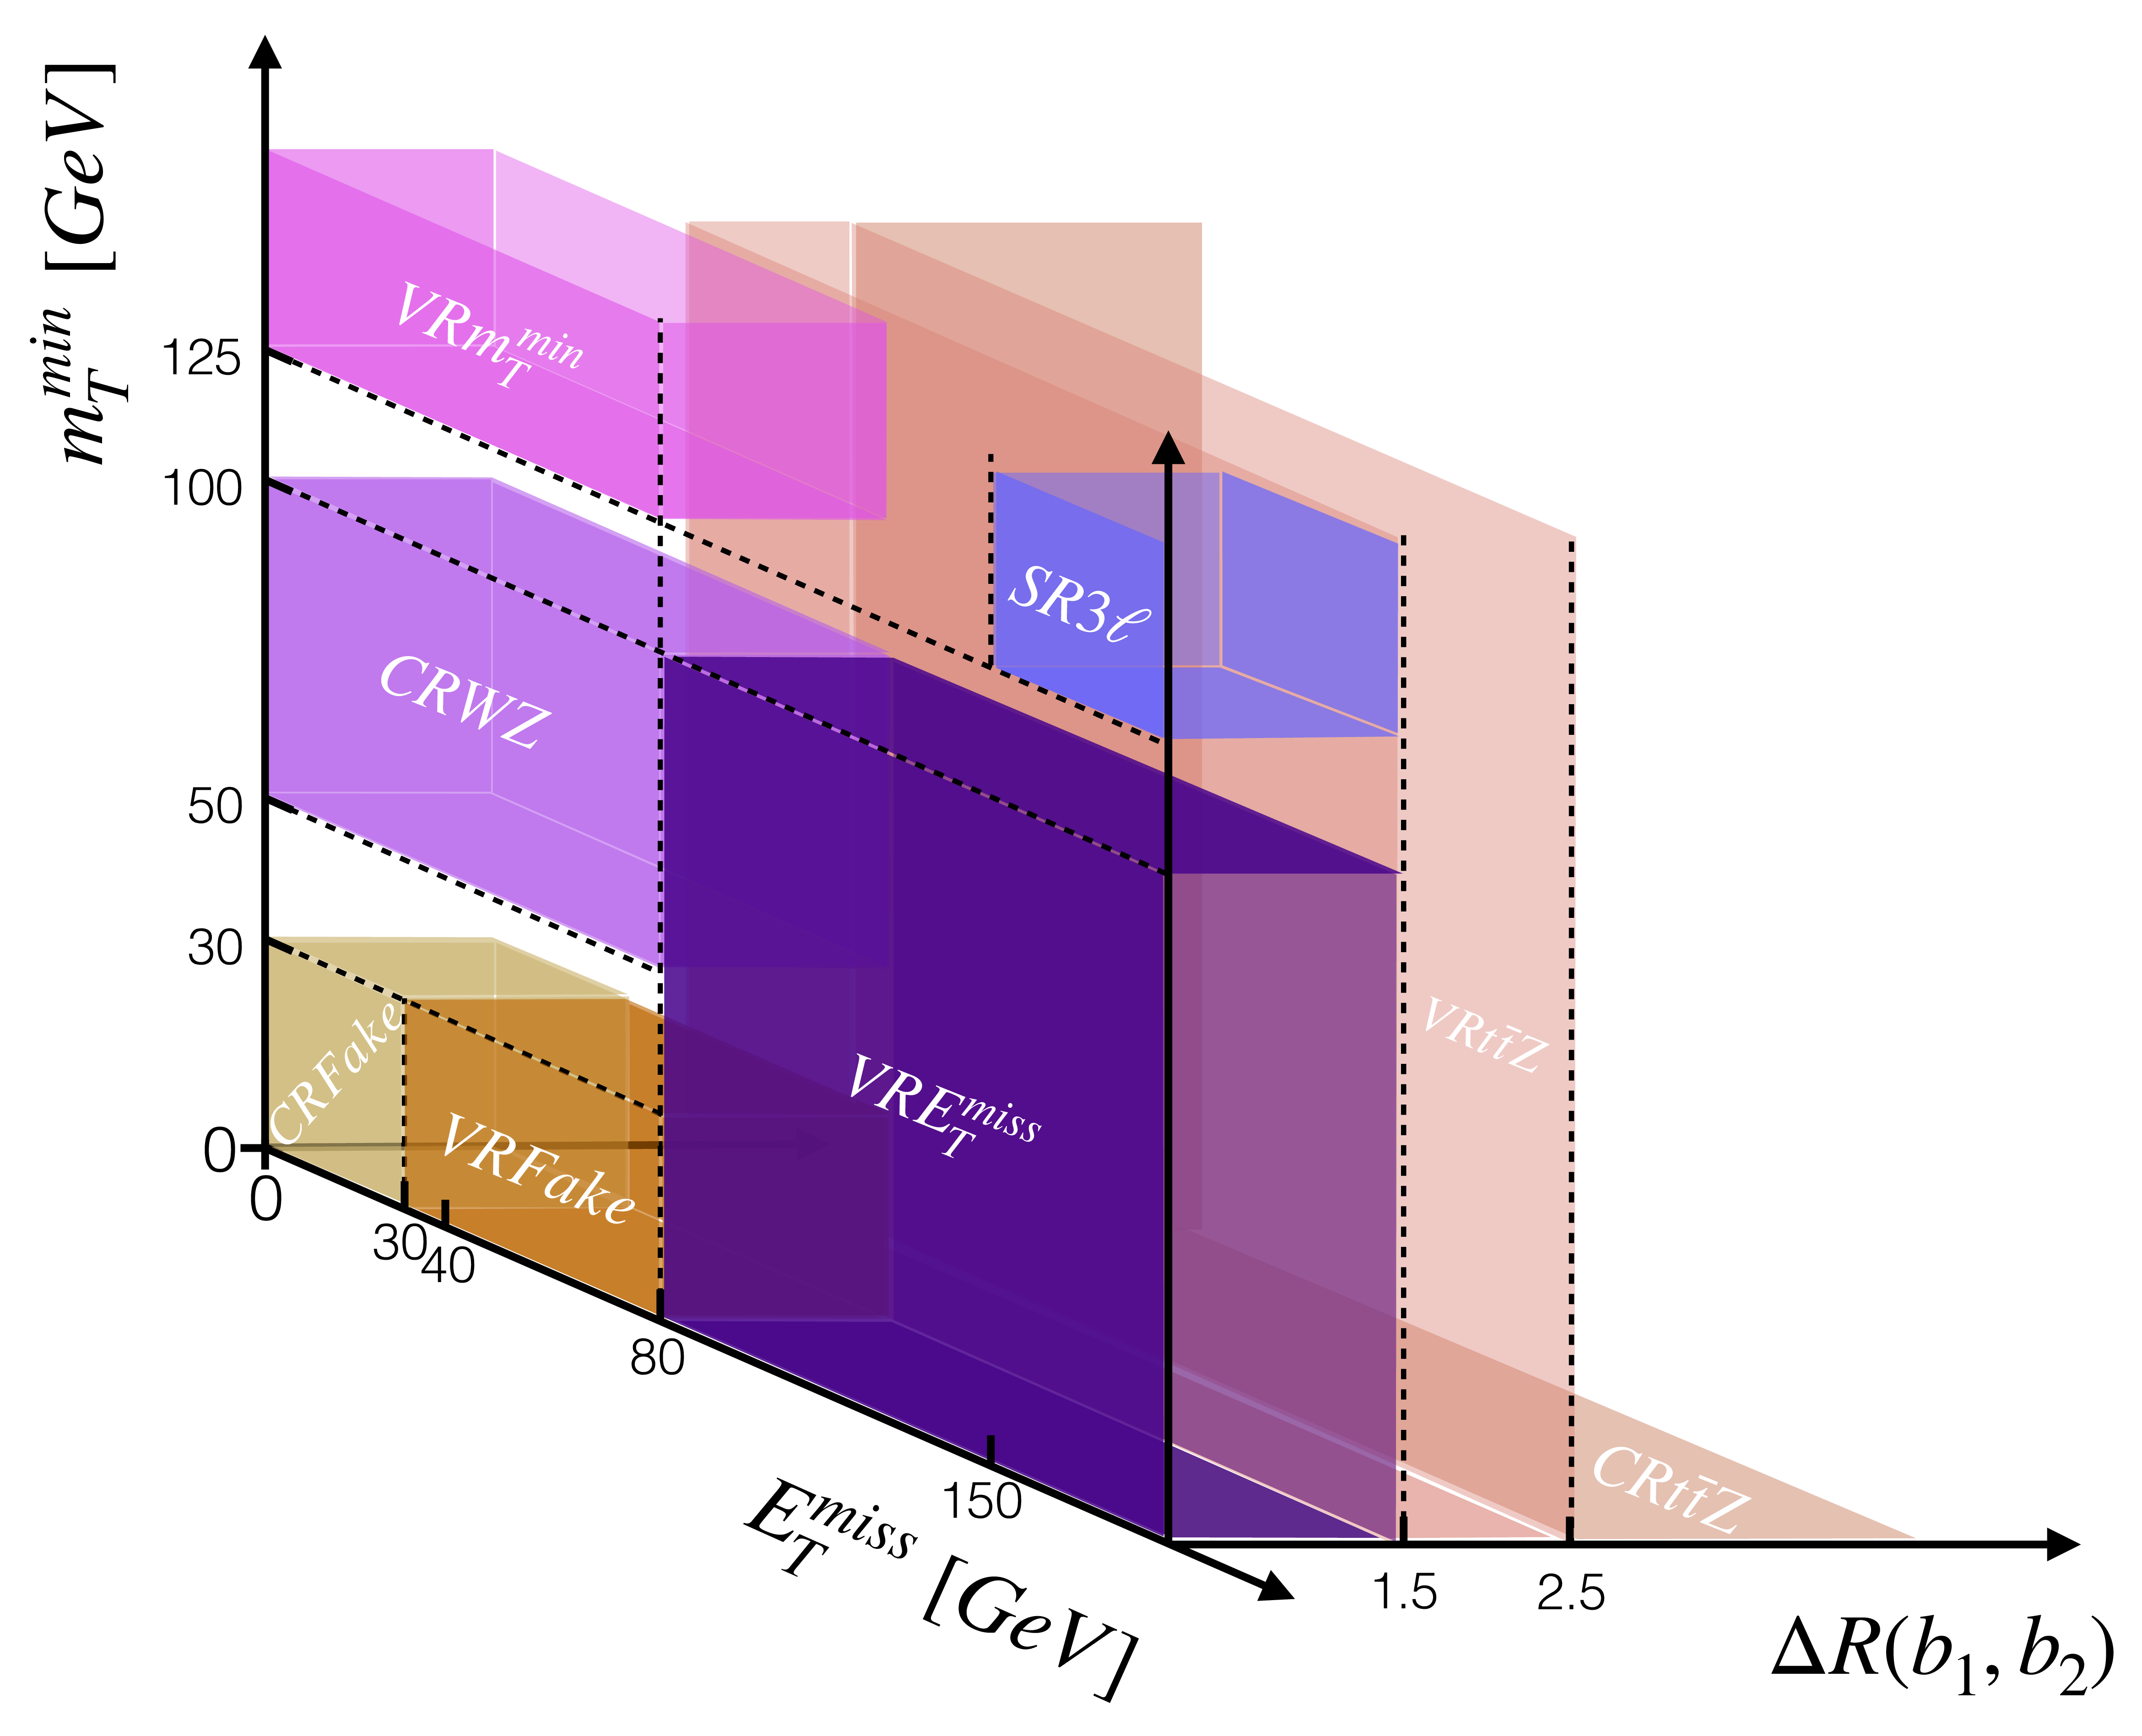
\includegraphics[width=0.98\textwidth]{figs/rpvthreel/3lregions.png}
    %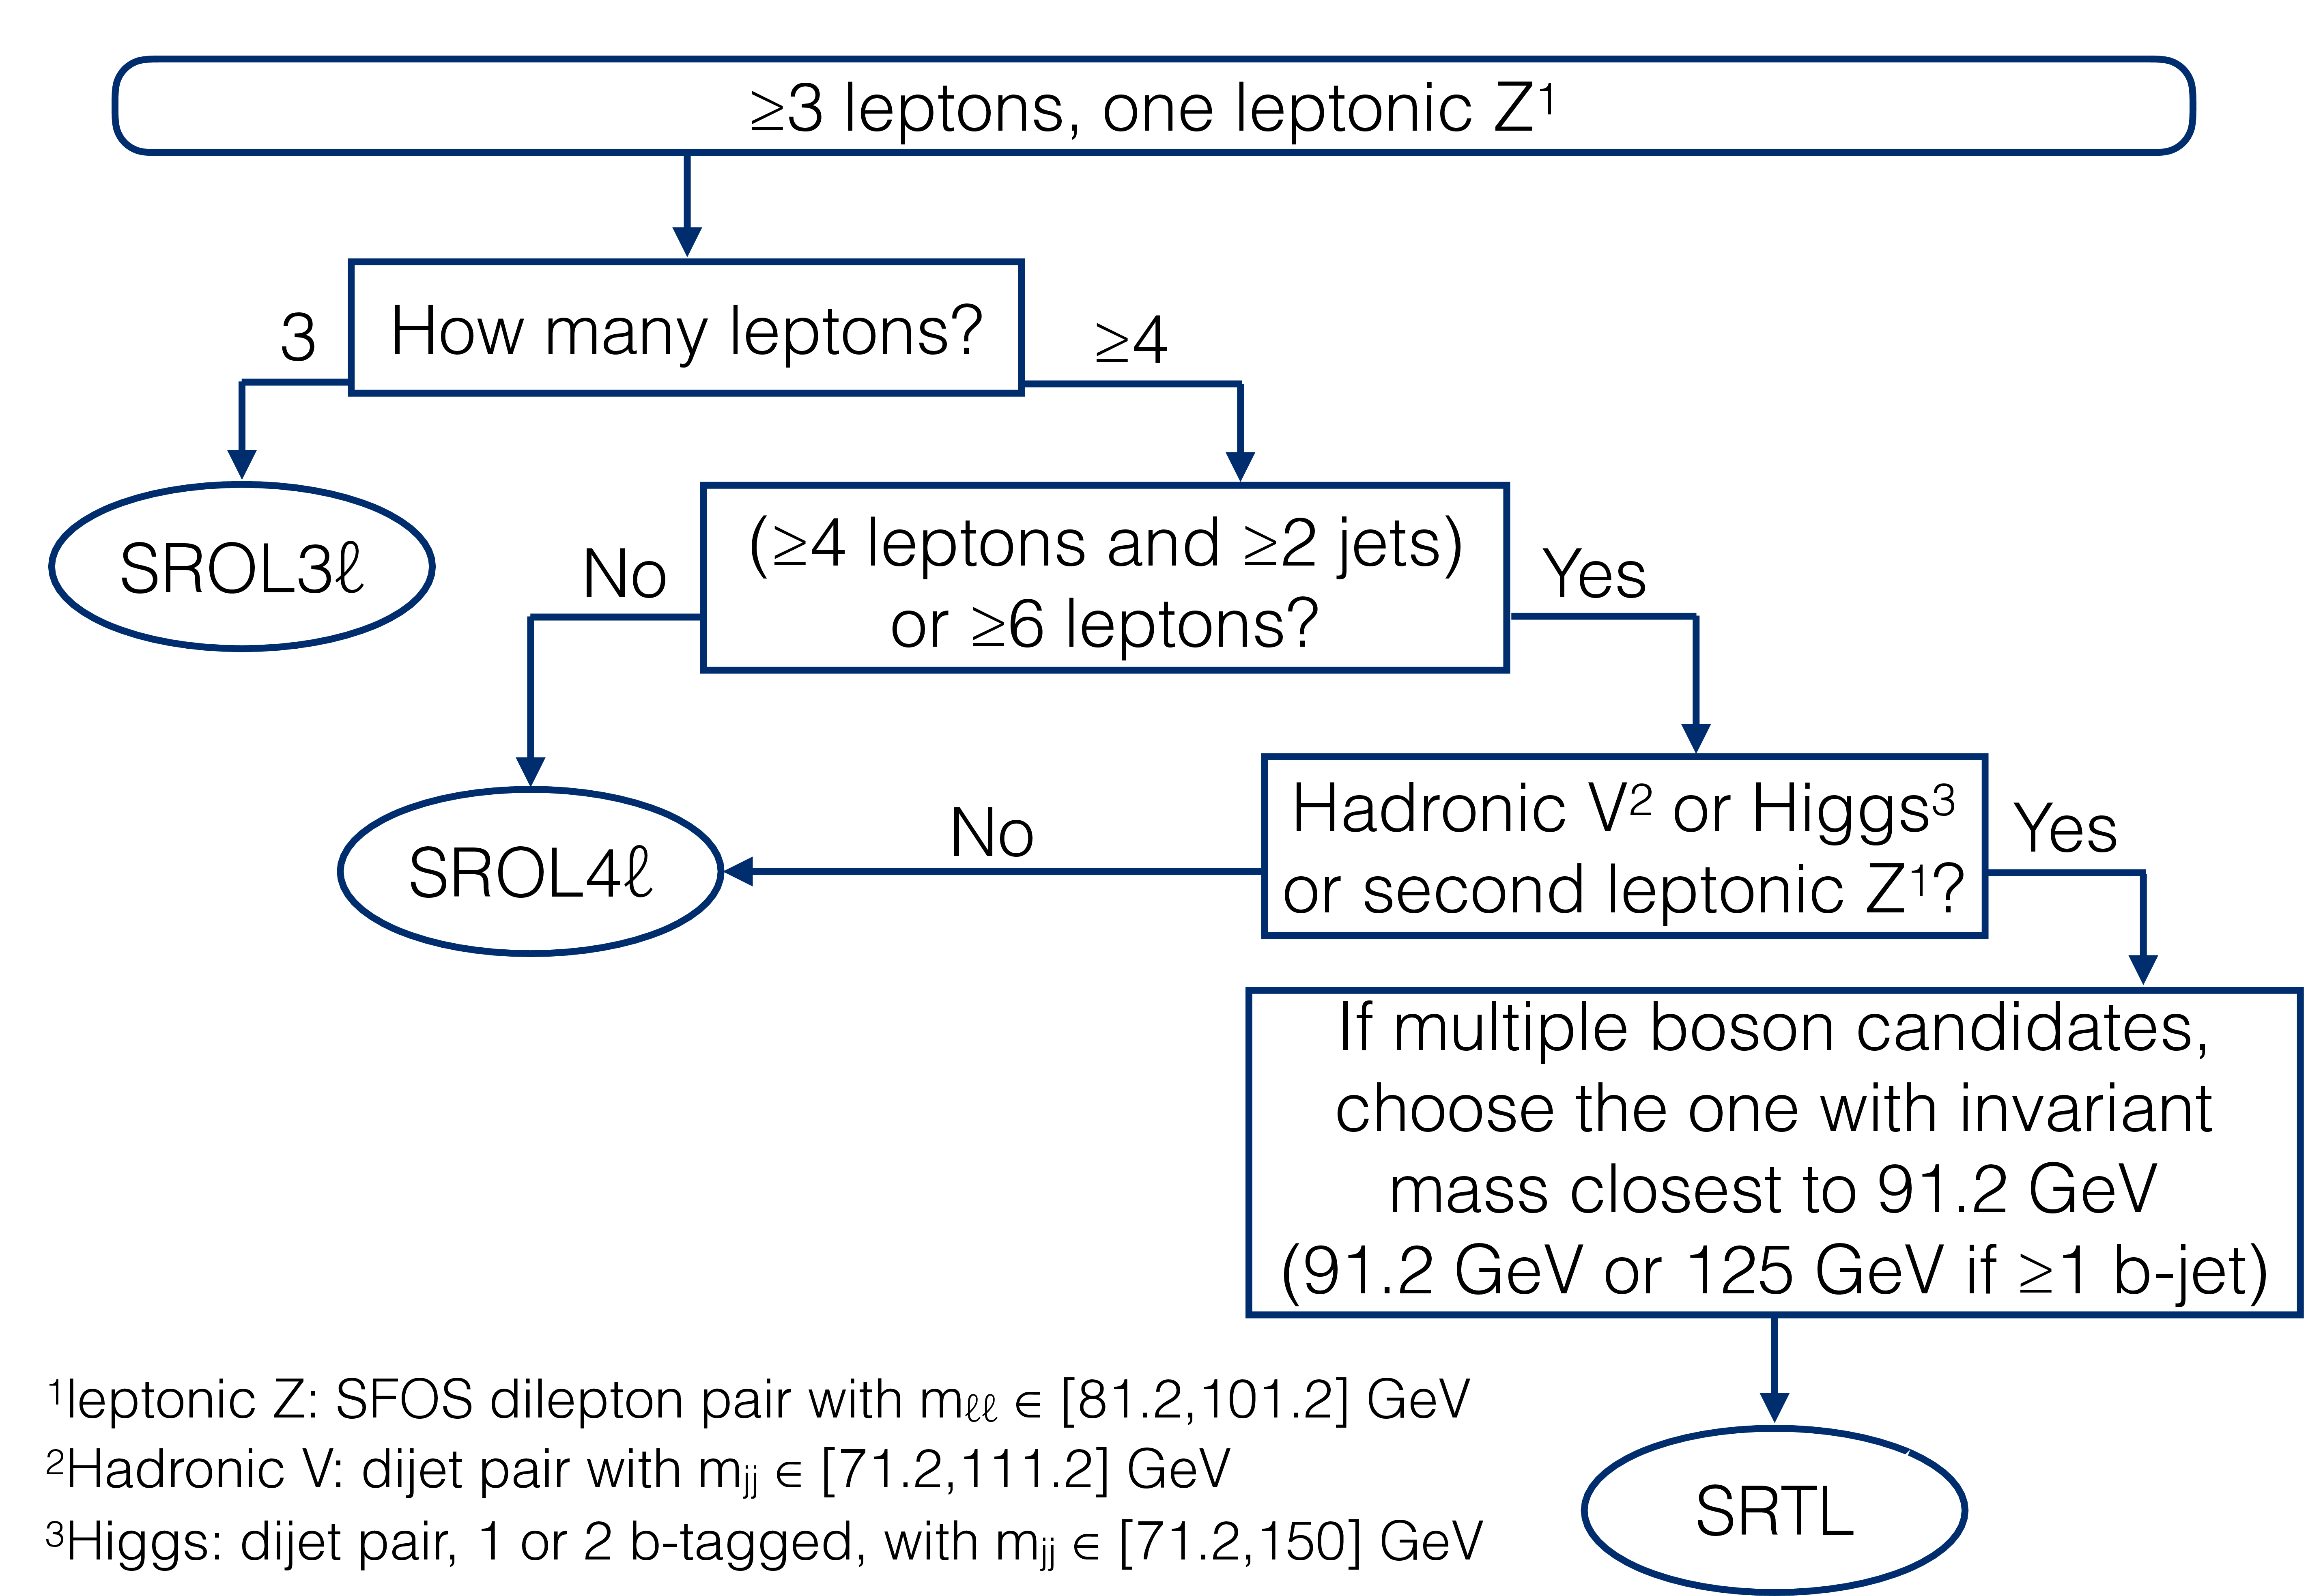
\includegraphics[width=0.98\textwidth]{figs/rpvthreel/regionCutflow.pdf}
  \end{center}
  \caption[Graphic depicting the orthogonality of the three lepton regions.]
          {Graphic depicting the orthogonality of the three lepton regions.
          Boxes without a side are unbounded in that direction in that variable.
          The full region definitions are summarized in Table \ref{tab:regions:regionBreakdown}}
   \label{fig:3lorthogonality}
\end{figure}
\begin{figure}[tbp]
    \centering
    \begin{subfigure}[b]{0.49\textwidth}
      \centering
      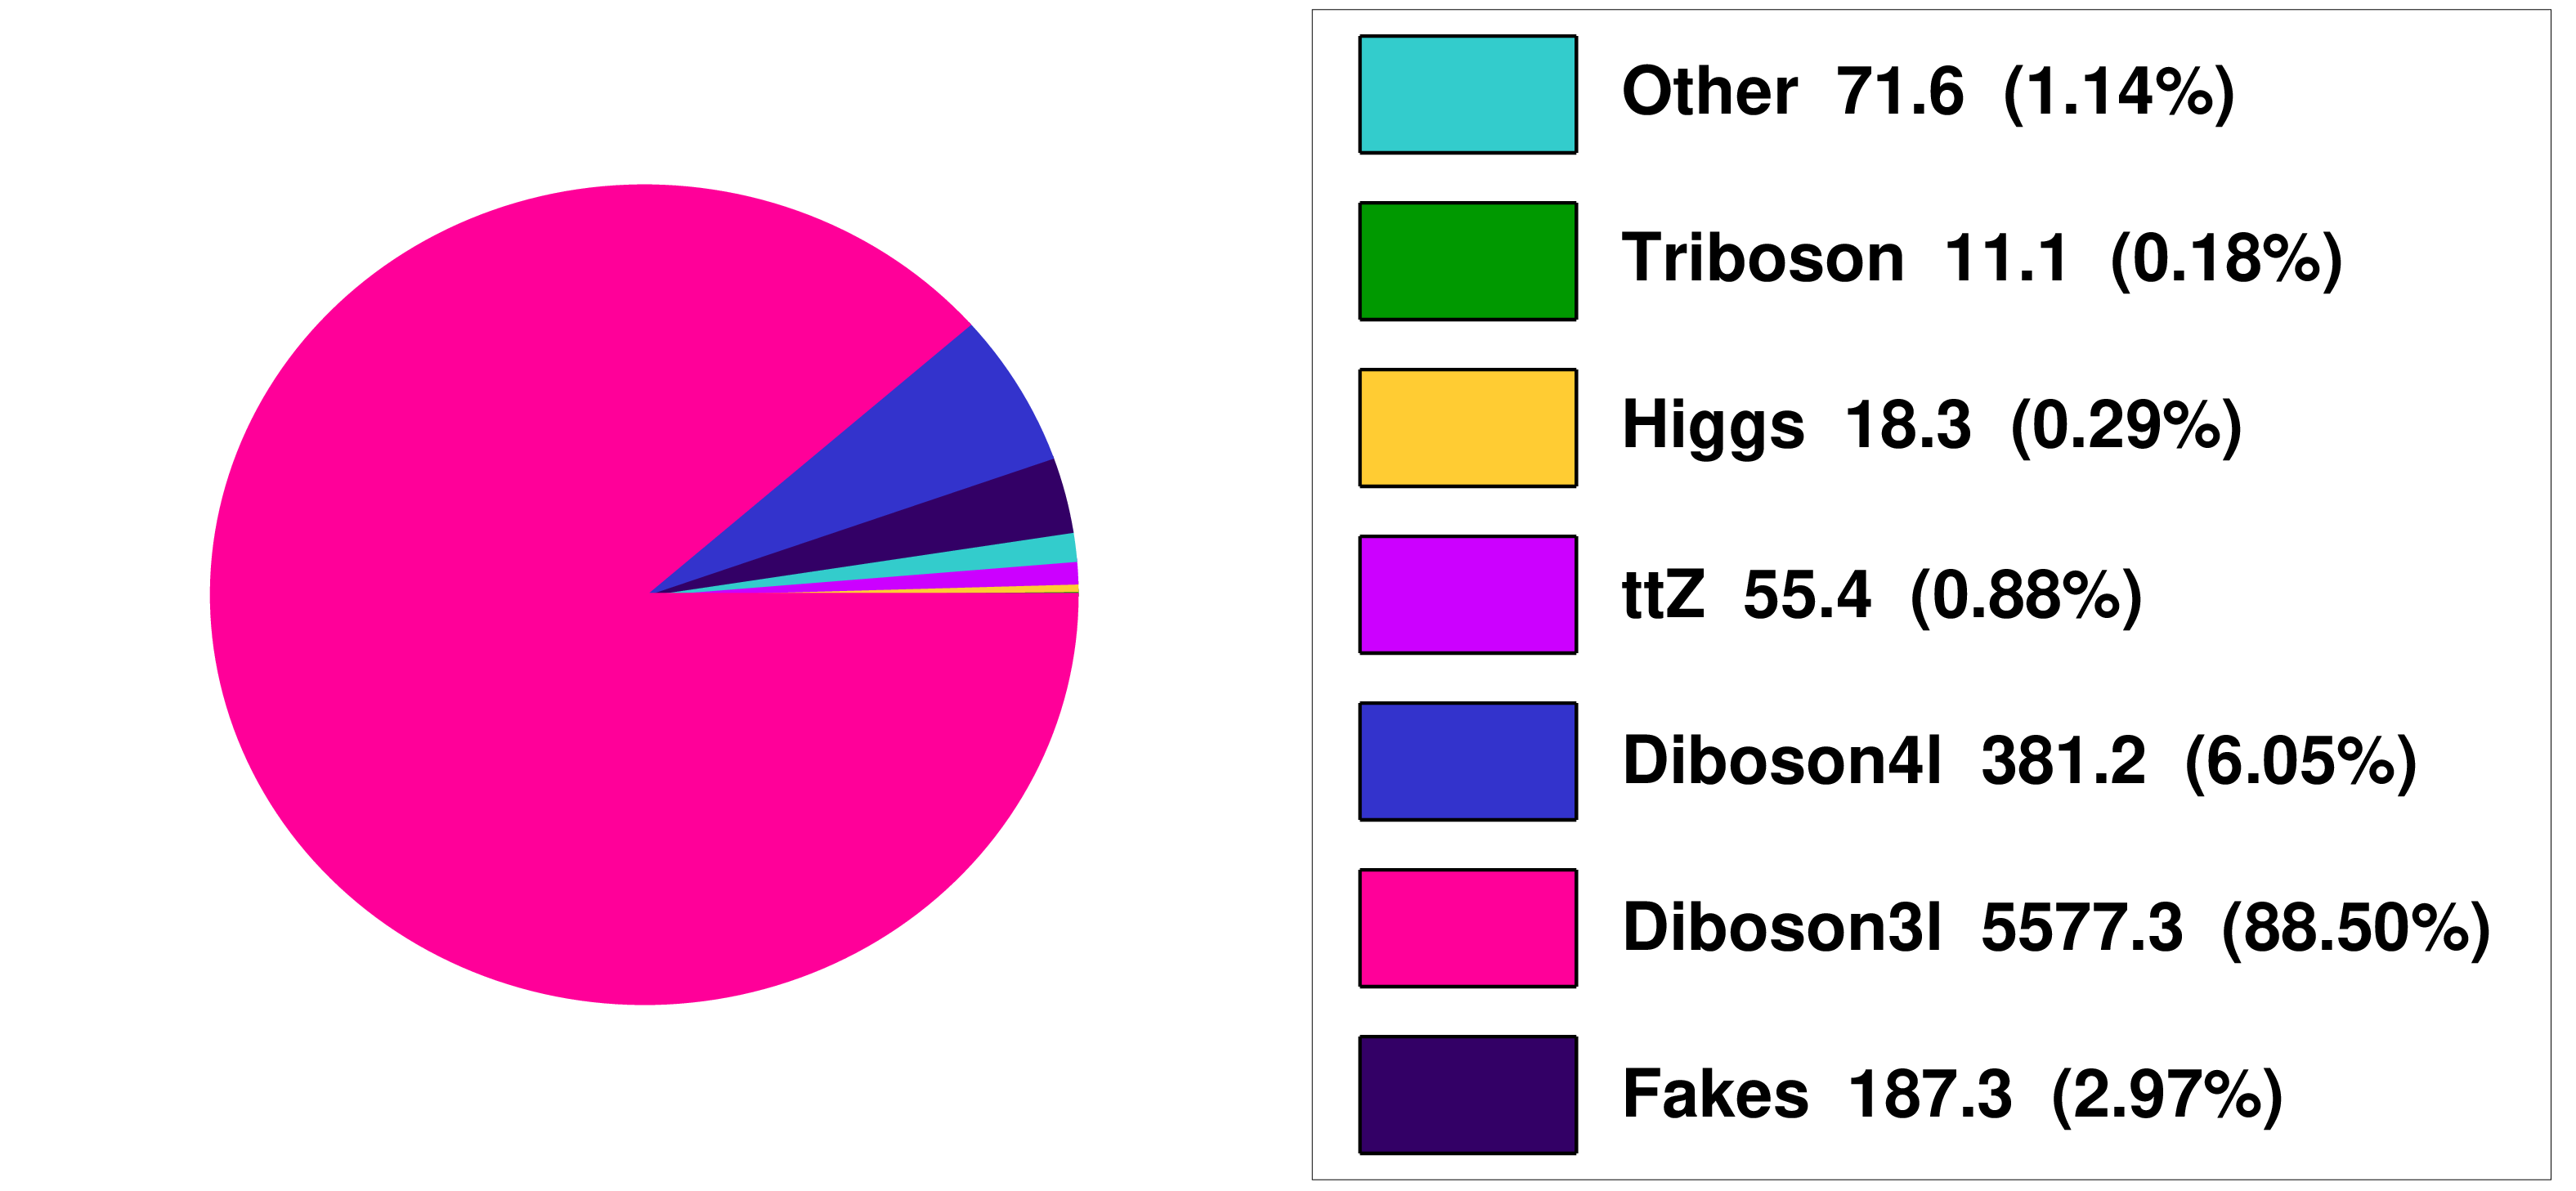
\includegraphics[width=0.98\textwidth]{figs/rpvthreel/CRWZ_yields.png}
      \caption{}
      \label{fig:CRWZ_yields}
    \end{subfigure}
    \hfill
    \begin{subfigure}[b]{0.49\textwidth}
      \centering
      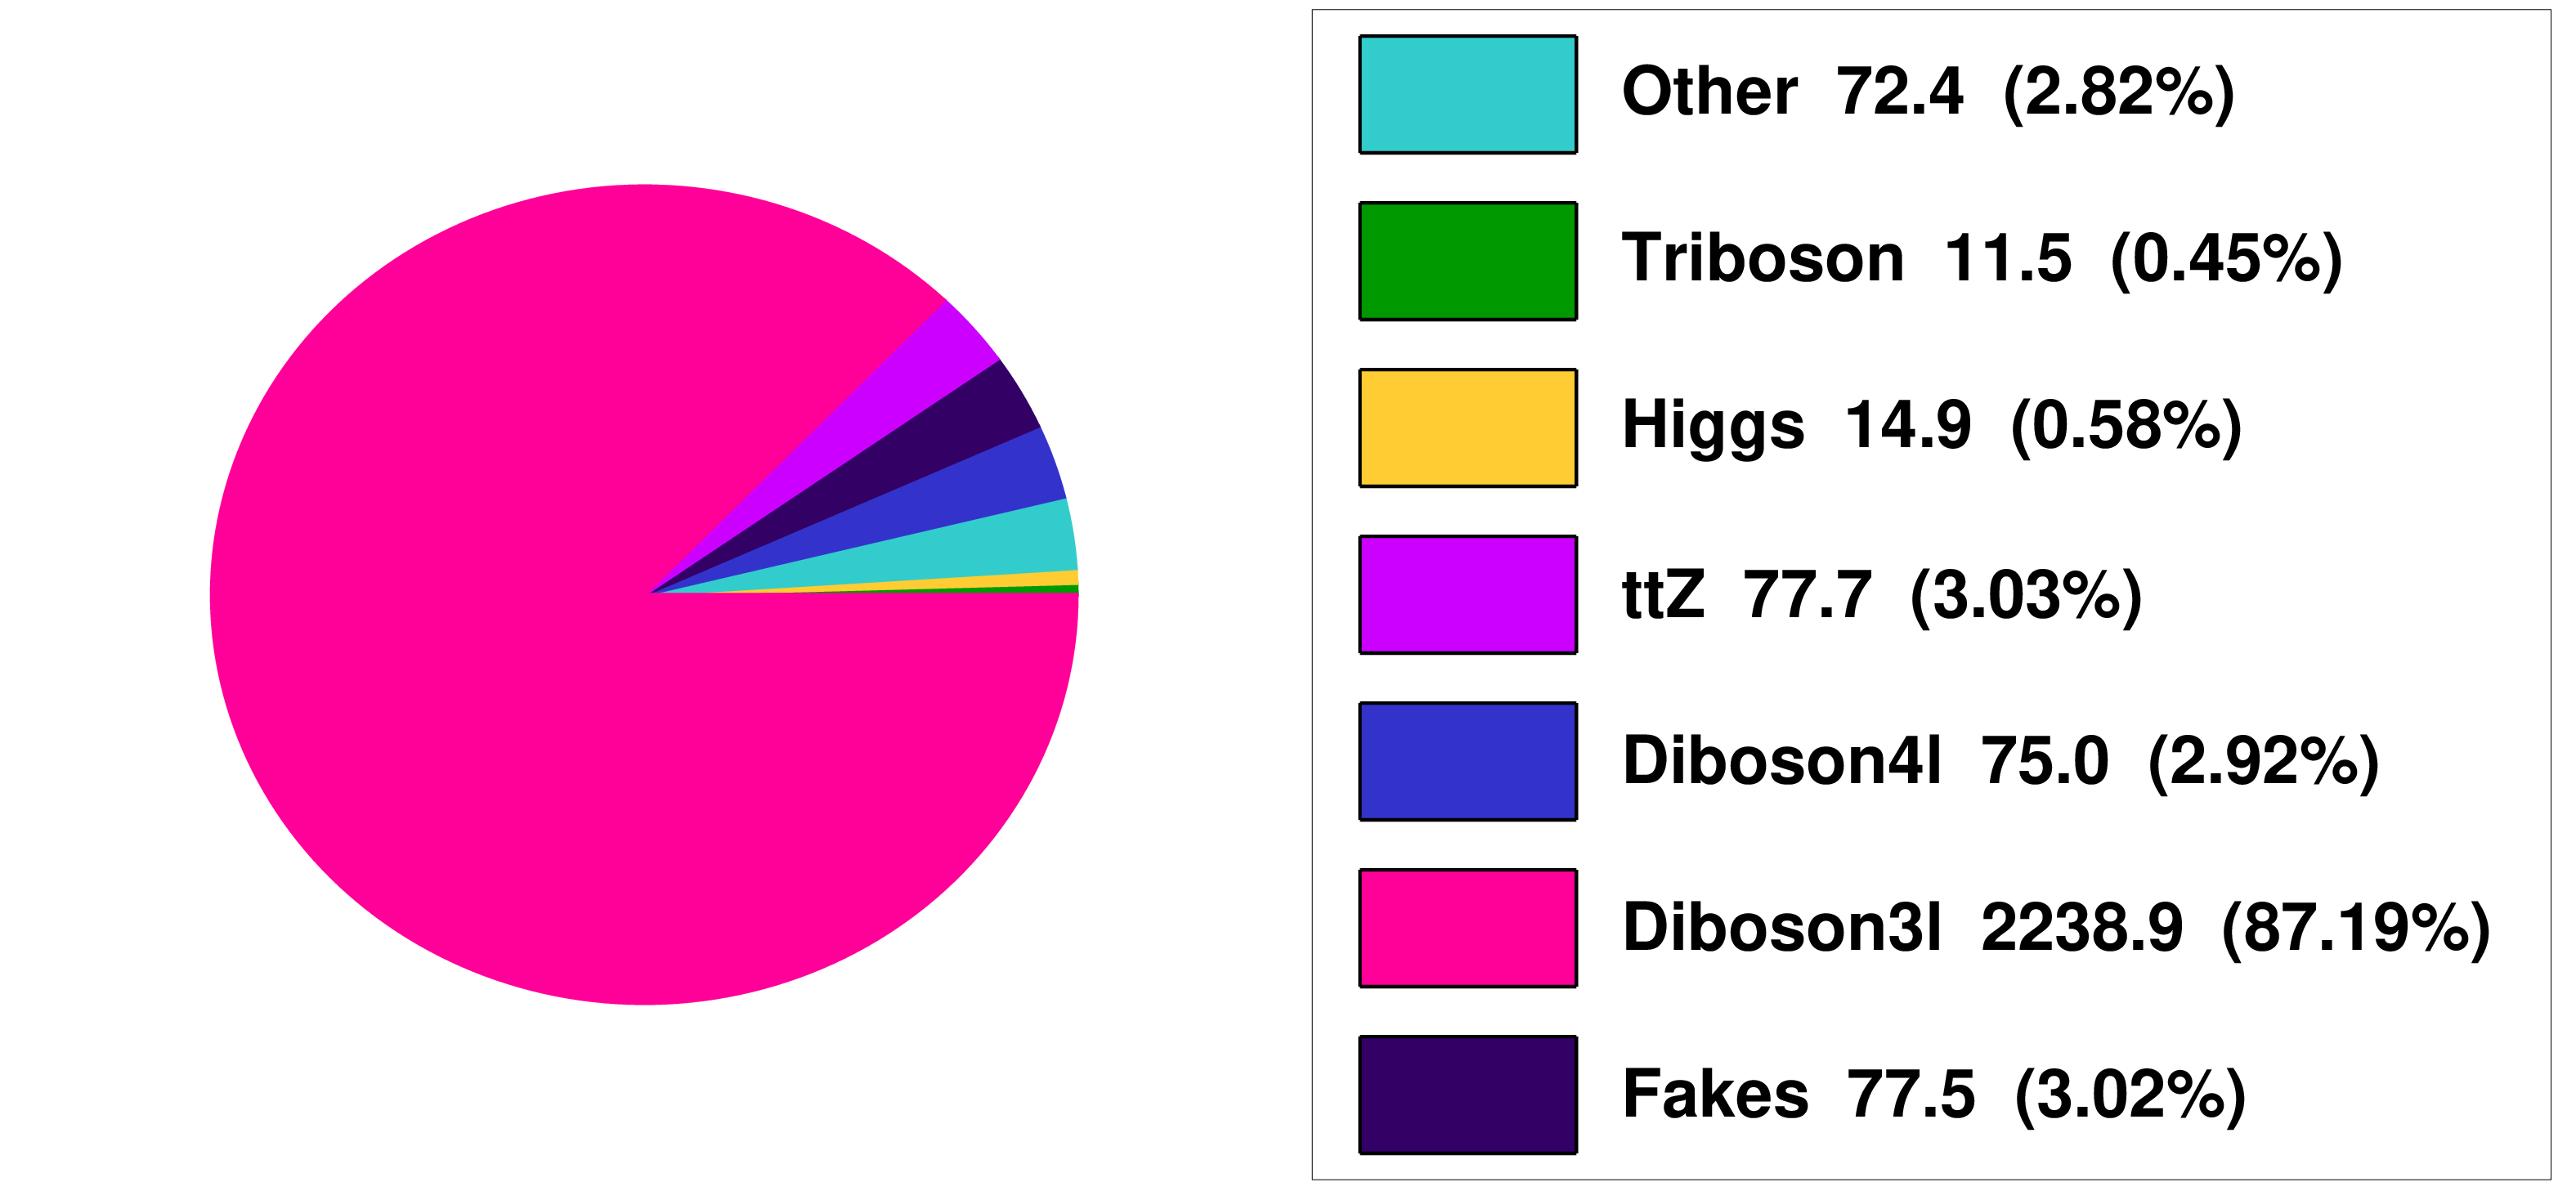
\includegraphics[width=0.98\textwidth]{figs/rpvthreel/VRMet_yields.png}
      \caption{}
      \label{fig:VRMet_yields}
    \end{subfigure}
    \hfill
    \begin{subfigure}[b]{0.49\textwidth}
      \centering
      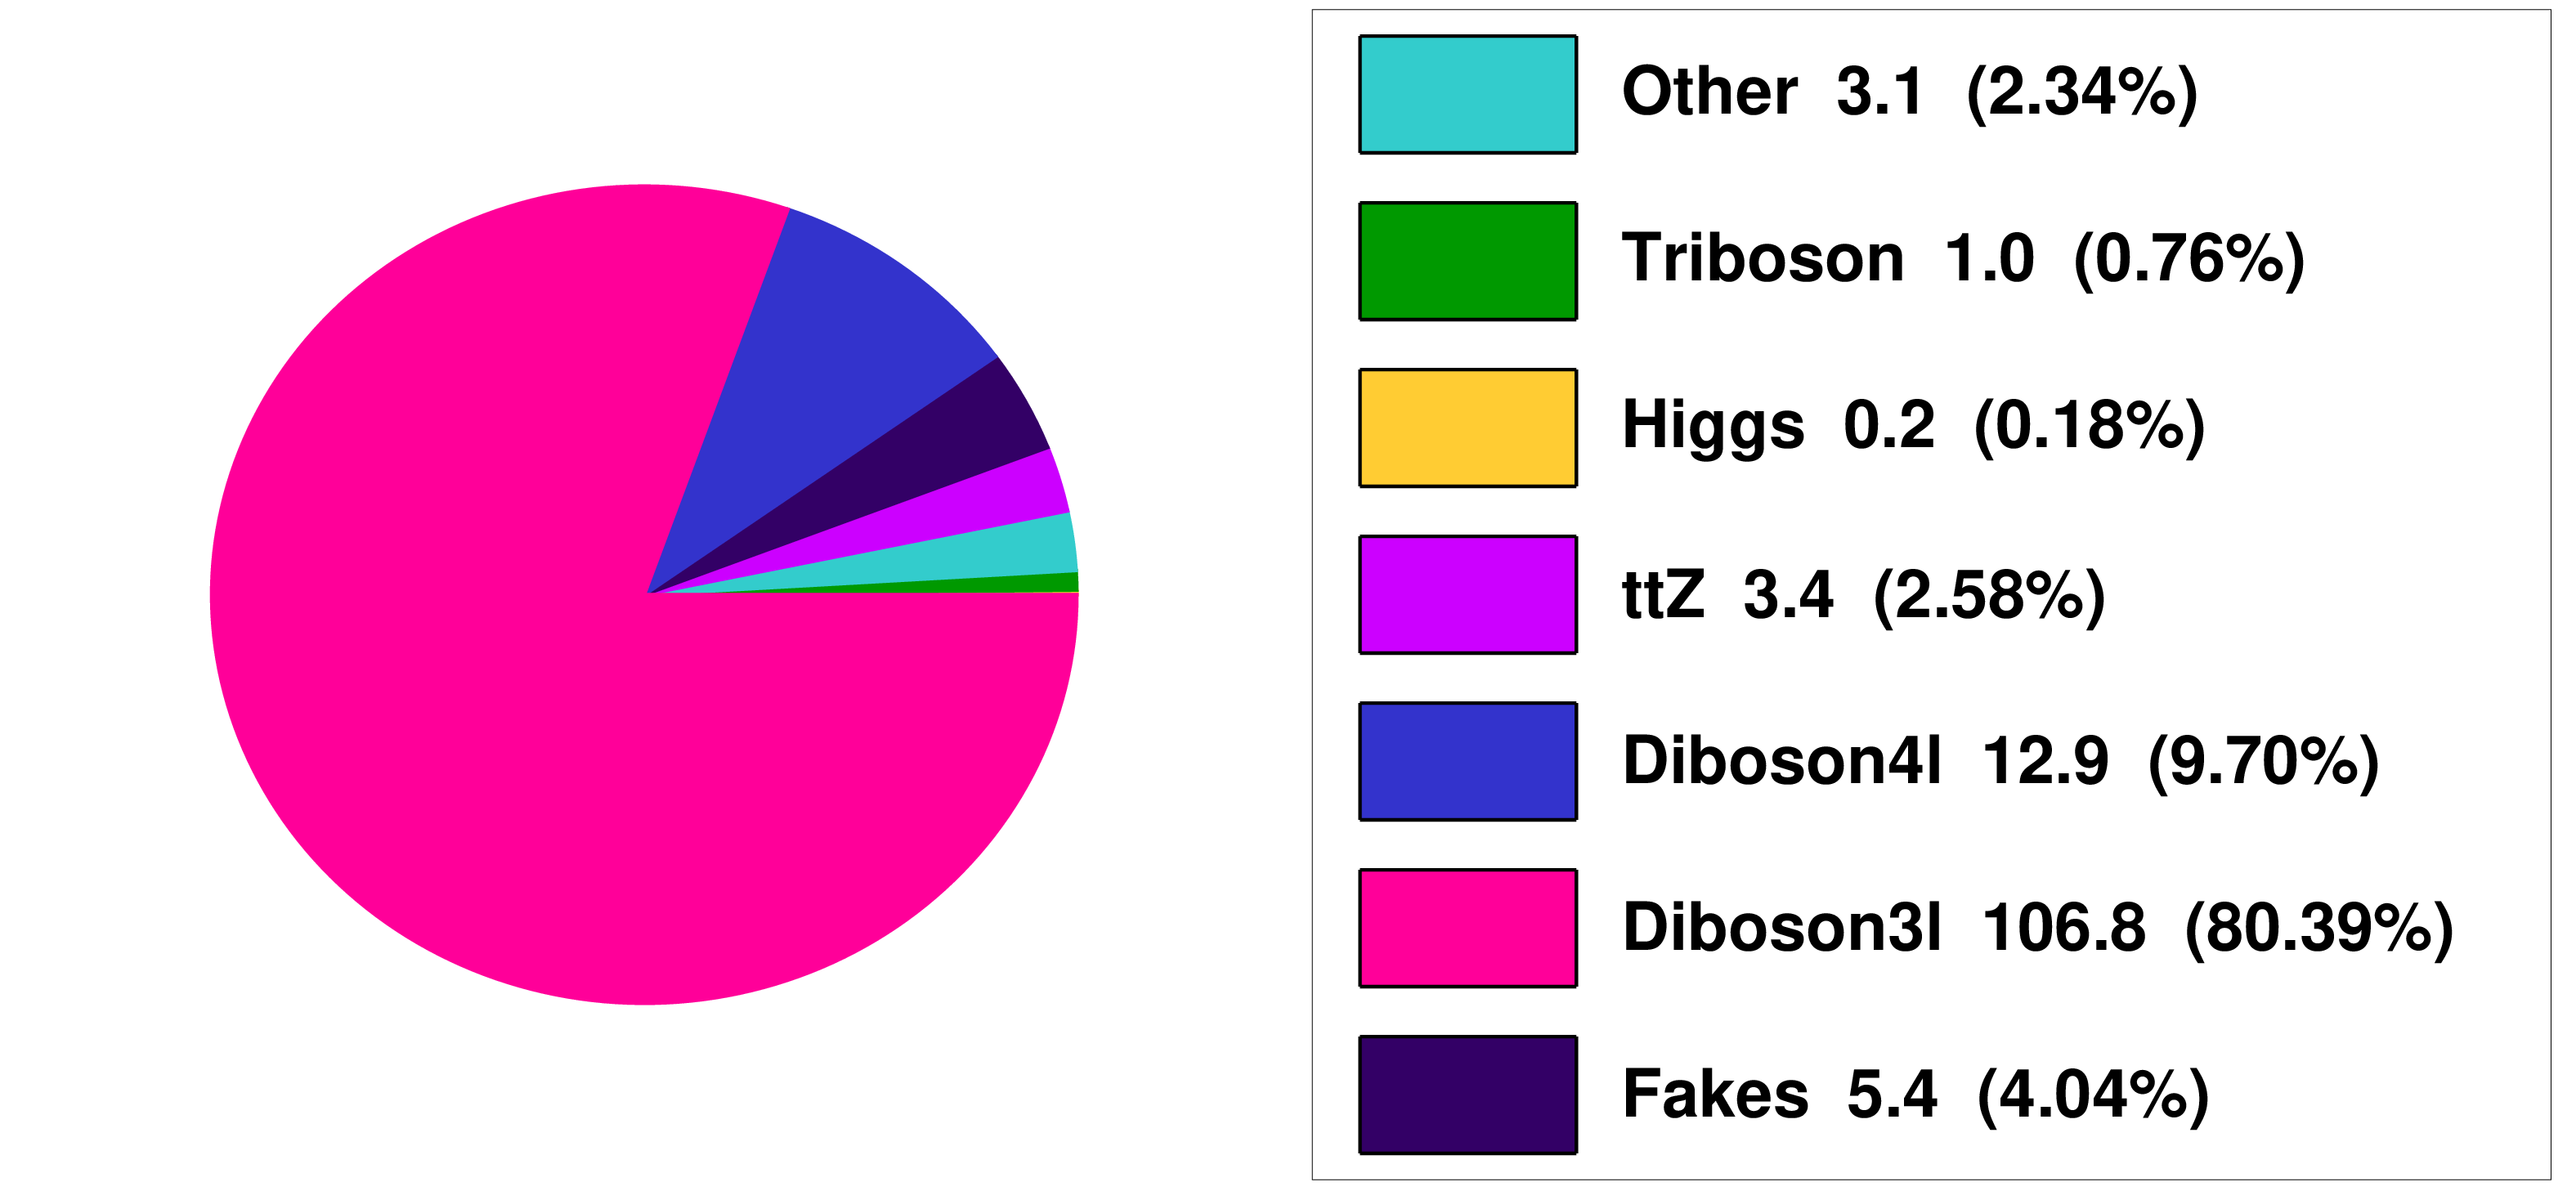
\includegraphics[width=0.98\textwidth]{figs/rpvthreel/VRmTmin_yields.png}
      \caption{}
      \label{fig:VRmTmin_yields}
    \end{subfigure}
  \caption[Expected yields of each background in \CRWZ, \VRmet and \VRmTmin, assuming 140 \ifb. No normalization factors are applied.]
          {Expected yields of each background in \CRWZ, \VRmet and \VRmTmin, assuming 140 \ifb. No normalization factors are applied.}
   \label{fig:CRVRWZ_yields}
\end{figure}
%i.e. this is a variable that can provide significant phase space separation between events with and with out a leptonically decaying \Wboson, i.e. expressly our \WZ background.
%Cuts on this variable combined with the pre-selection three lepton and of a SFOS lepton pair consistent with the \Zboson\ mass creates a very pure selection of \WZ events.
%It is still then possible to increase the purity even further, as well as reduce signal contamination, by requiring the \met~ cut, \met~ $ < 80~\gev$.

\subsubsection{Handling Backgrounds: \ZZ}
\label{sec:crzz}
Regions designed to constrain \ZZ, which dominates both the four lepton regions \SRFour and \SRFR, are required to have two SFOS lepton pairs.
This single requirement already gives a very pure \ZZ region.
% Show plot?
The region is then further subdivided into CR and VR regions differentiated by the requirement on the mass window of the second reconstructed \Zboson\ mass, $ m_{ll,2} $.
The stricter requirement of the two is a window within 5~\gev of the \Zboson\ mass which defines the control region \CRZZ.
For \VRZZ a looser window requirement is defined within 20~\gev, which does not include the \CRZZ window in order to maintain orthogonality.
The expected yields in the control and validation regions for \ZZ are shown in Figure~\ref{fig:CRVRZZ_yields}.
The $m_{ll,2}$ distribution which contains both \CRZZ and \VRZZ can be seen in Figure \ref{fig:mll2ZZ} where good agreement is seen between data and the post-fit background estimates.
Events for which one $Z$ decays into a pair of $\tau$-leptons that both then subsequently decay leptonically are included in this validation region.
Good modeling in the three-lepton regions is also expected for such \ZZ events when only one $\tau$-lepton decays leptonically,
although this process is strongly suppressed by the \met\ and \mTmin requirements.
Again a cut of \dRbb$>$~1.5 is made to guarantee orthogonality to \ttZ regions.
The full definition of cuts for this region are shown in the region summary Table \ref{tab:regions:regionBreakdown} and illustrated in Figure~\ref{fig:4lorthogonality}. 
\begin{figure}[tbp]
  \begin{center}
    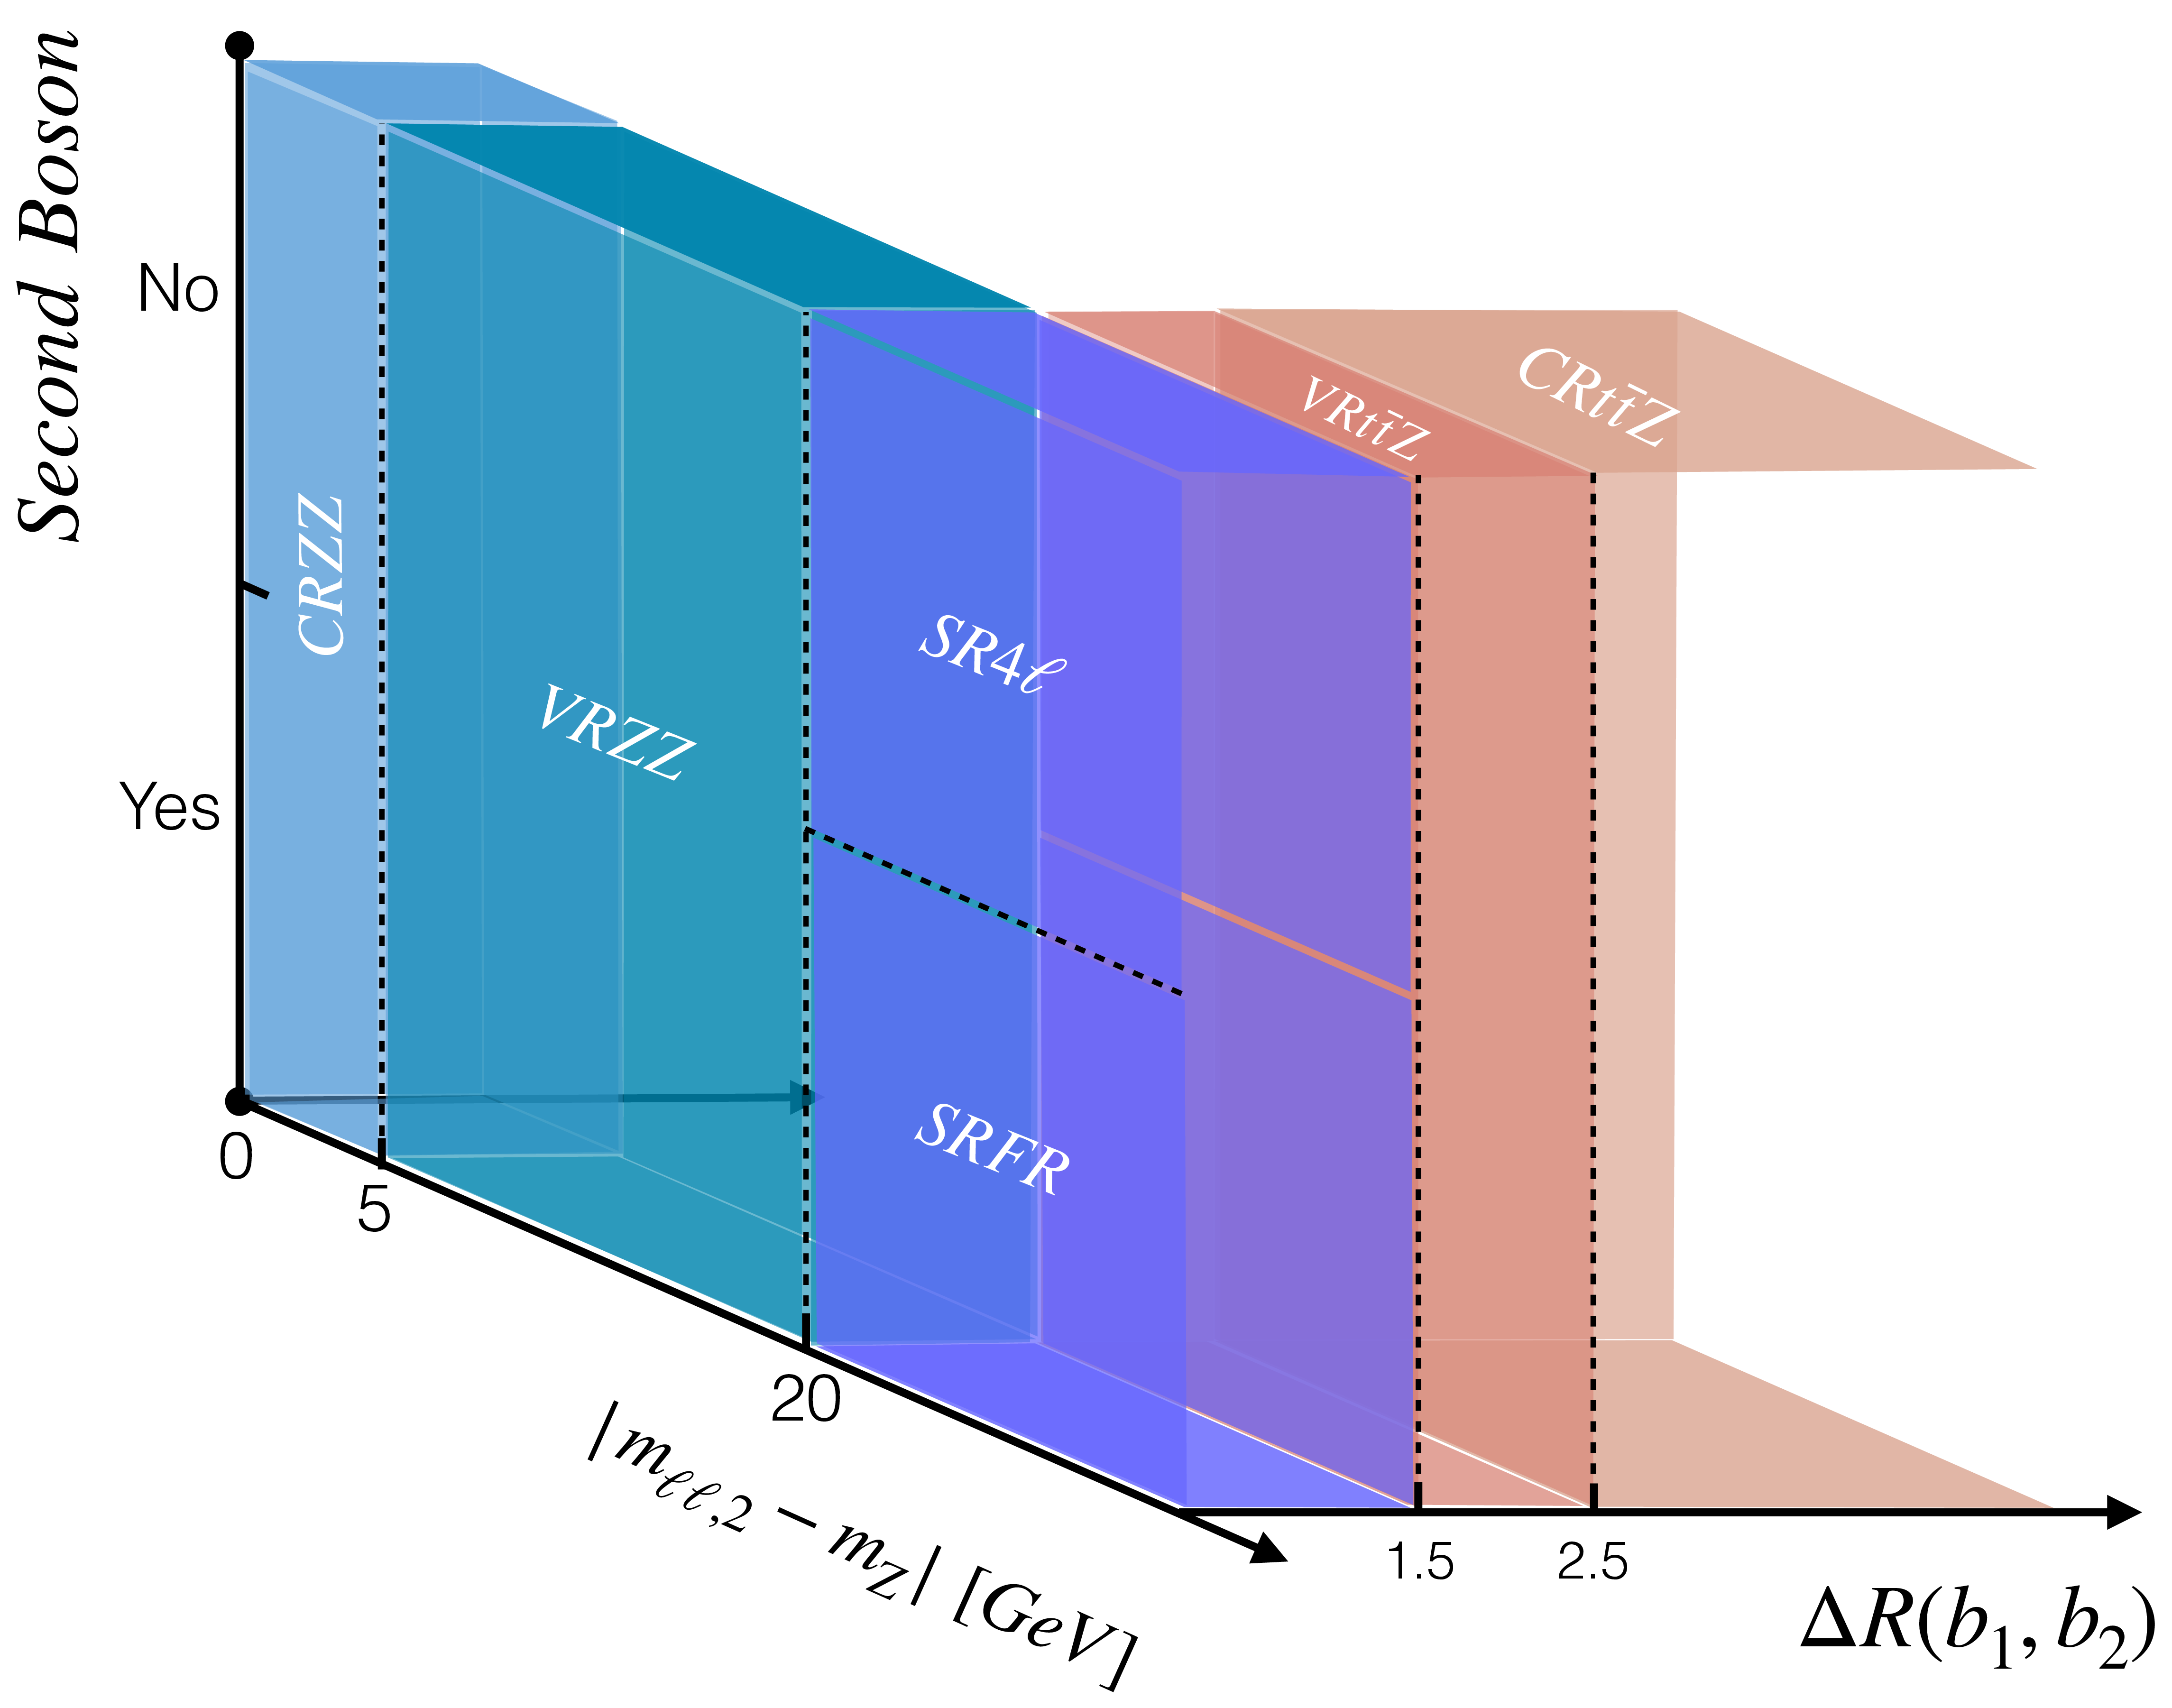
\includegraphics[width=0.98\textwidth]{figs/rpvthreel/4lregions.png}
  \end{center}
  \caption[Graphic depicting the orthogonality of the four lepton regions.]
          {Graphic depicting the orthogonality of the four lepton regions.
          Boxes without a side are unbounded in that direction in that variable.
          The full region definitions are summarized in Table \ref{tab:regions:regionBreakdown}}
          \label{fig:4lorthogonality}
\end{figure}
\begin{figure}[tbp]
    \centering
    \begin{subfigure}[b]{0.49\textwidth}
      \centering
      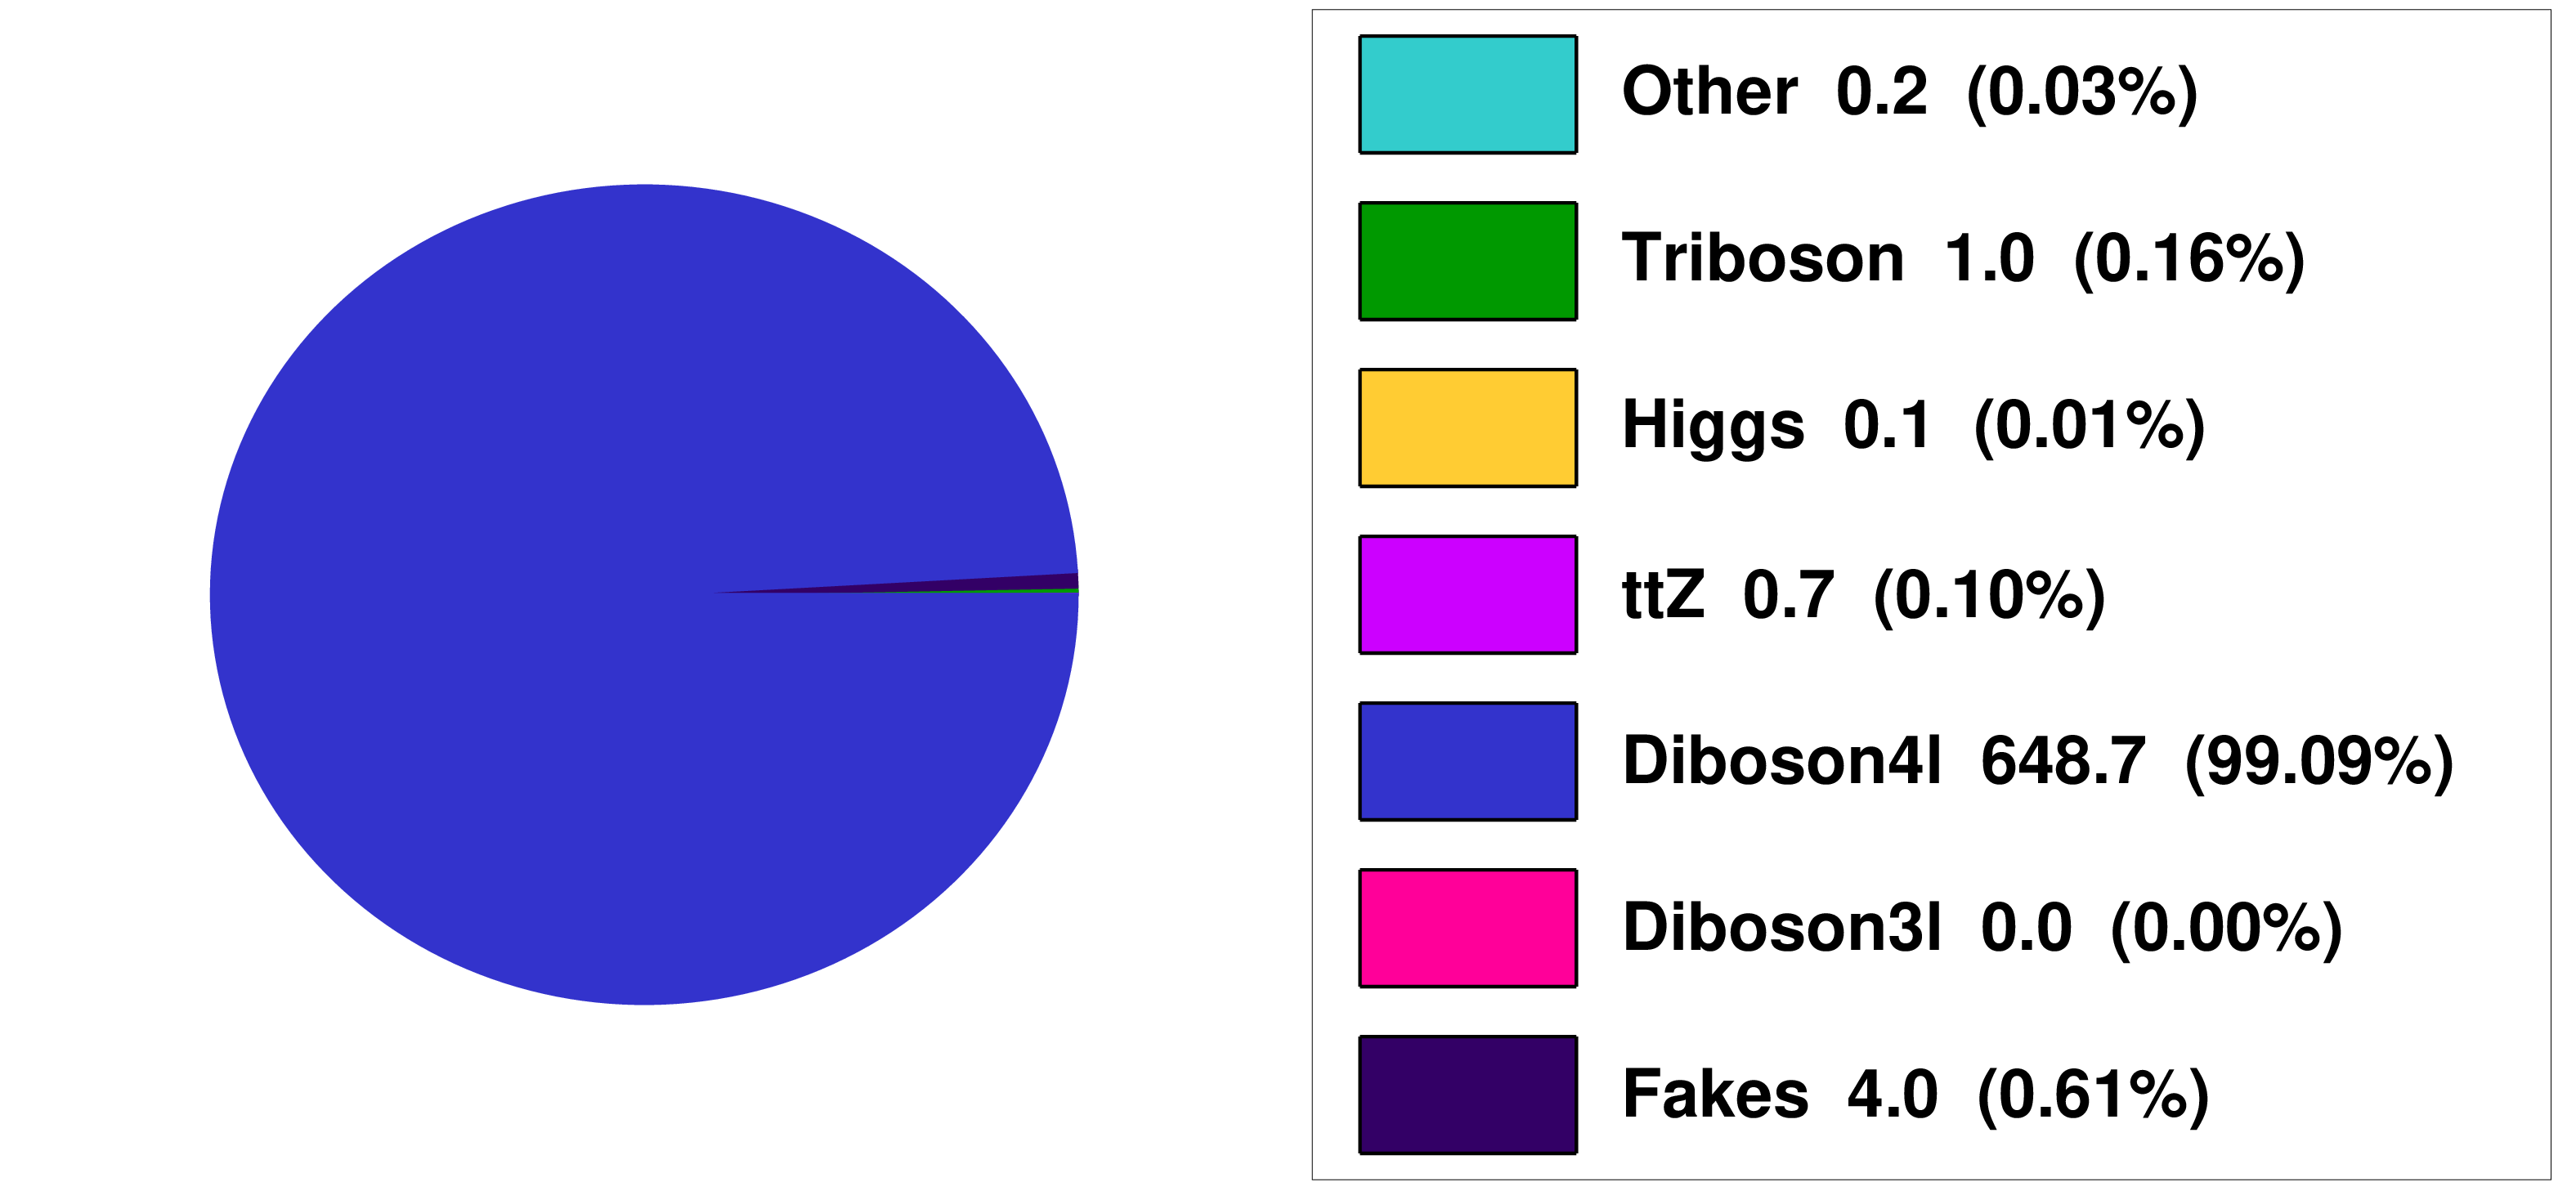
\includegraphics[width=0.98\textwidth]{figs/rpvthreel/CRZZ_yields.png}
      \caption{}
      \label{fig:CRZZ_yields}
    \end{subfigure}
    \hfill
    \begin{subfigure}[b]{0.49\textwidth}
      \centering
      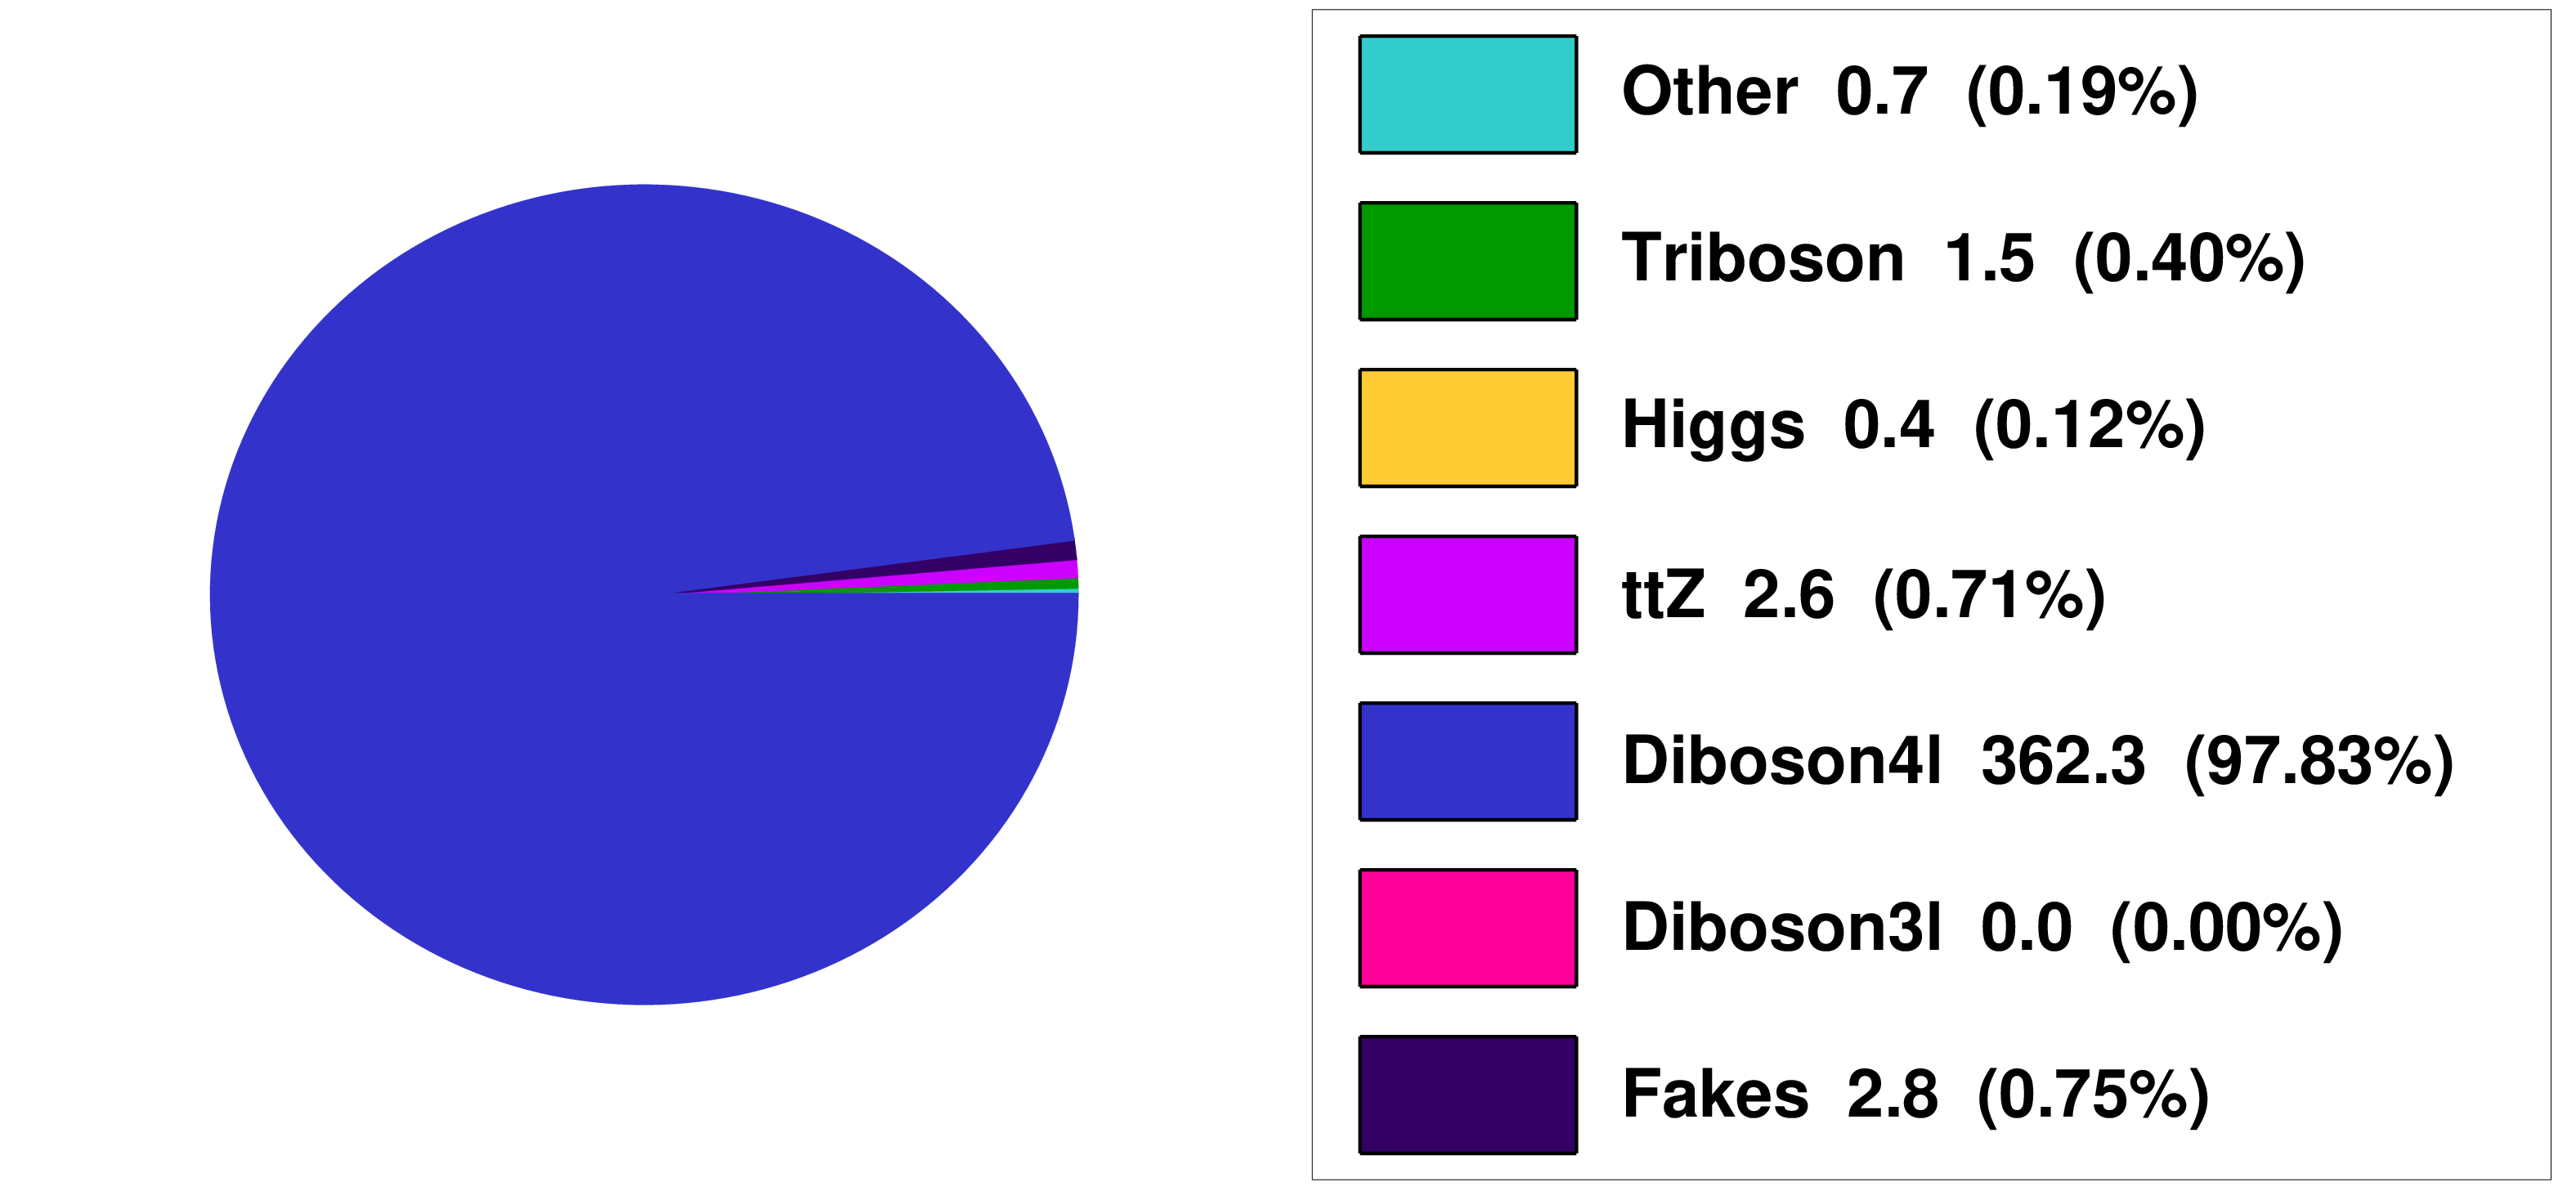
\includegraphics[width=0.98\textwidth]{figs/rpvthreel/VRZZ_yields.png}
      \caption{}
      \label{fig:VRZZ_yields}
    \end{subfigure}
  \caption[Expected yields of each background in \CRZZ and \VRZZ, assuming 140 \ifb. No normalization factors are applied.]
          {Expected yields of each background in \CRZZ and \VRZZ, assuming 140 \ifb. No normalization factors are applied.}
   \label{fig:CRVRZZ_yields}
\end{figure}

\subsubsection{Handling Backgrounds: \ttZ}
\label{sec:crttz}
The last dominant background, \ttZ, contributes via a leptonically decaying \Zboson\ and two top quarks in which one or both decay leptonically.
While \ttZ is primarily a major background in \SRFR the it is useful to construct the region such that it includes three lepton events as well in order to improve statistics in the region as well as to be able to extrapolate over number of leptons in the fit.
Many variations of cuts on standard variables such as \met\ and $b$-jet multiplicity were studied but the underlying physics of \ttbar decays, which heavily favor final states with two $b$-quarks, resulted in the best separation with reasonable CR purity and acceptable statistics.
Thus, a requirement of $N_{b-\textrm{jet}}\geq2$ is imposed along with a \FourlTwoZ veto in order to reduce contributions from \ZZ.
We can then go further by taking advantage of the expected large angular separation of the two b-quarks coming from \ttbar to further purify the \ttZ regions as well as to apply a blanket orthogonality requirement against all other regions.
To get a handle on this separation the \dr between the two highest \pt $b$-tagged jets in the event is defined as the variable \dRbb.
Figure \ref{fig:dRbb_PreSel} shows the. expected distribution from background processes as well as a few representative signal points in \dRbb at pre-selection, i.e. the baseline selection with three or more leptons.
From the linear plot in Figure \ref{fig:dRbb_Presel_lin} it is clear that \ttZ events favor a large angular separation between $b$-jets and the peak at \dRbb $\approx \pi$ is consistent with back-to-back production of \ttbar.
The relative high purity of \ttZ events through out this distribution invites us to compose a CR and VR.
Cuts of $1.5<$\dRbb$\leq2.5$ and \dRbb$\geq2.5$ were found to be optimal for \VRttZ and \CRttZ respectively.
While the region of \dRbb$\leq1.5$ is reserved for all other regions and therefore imposes orthogonality everywhere.
Yields in \VRttZ and \CRttZ are shown in Figure \ref{fig:ttZ_yields}.
The full definition of cuts for this region are shown in the region summary Table~\ref{tab:regions:regionBreakdown} and illustrated in Figures~\ref{fig:3lorthogonality} and \ref{fig:4lorthogonality}.
\begin{figure}[tbp]
    \centering
    \begin{subfigure}[b]{0.49\textwidth}
      \centering
      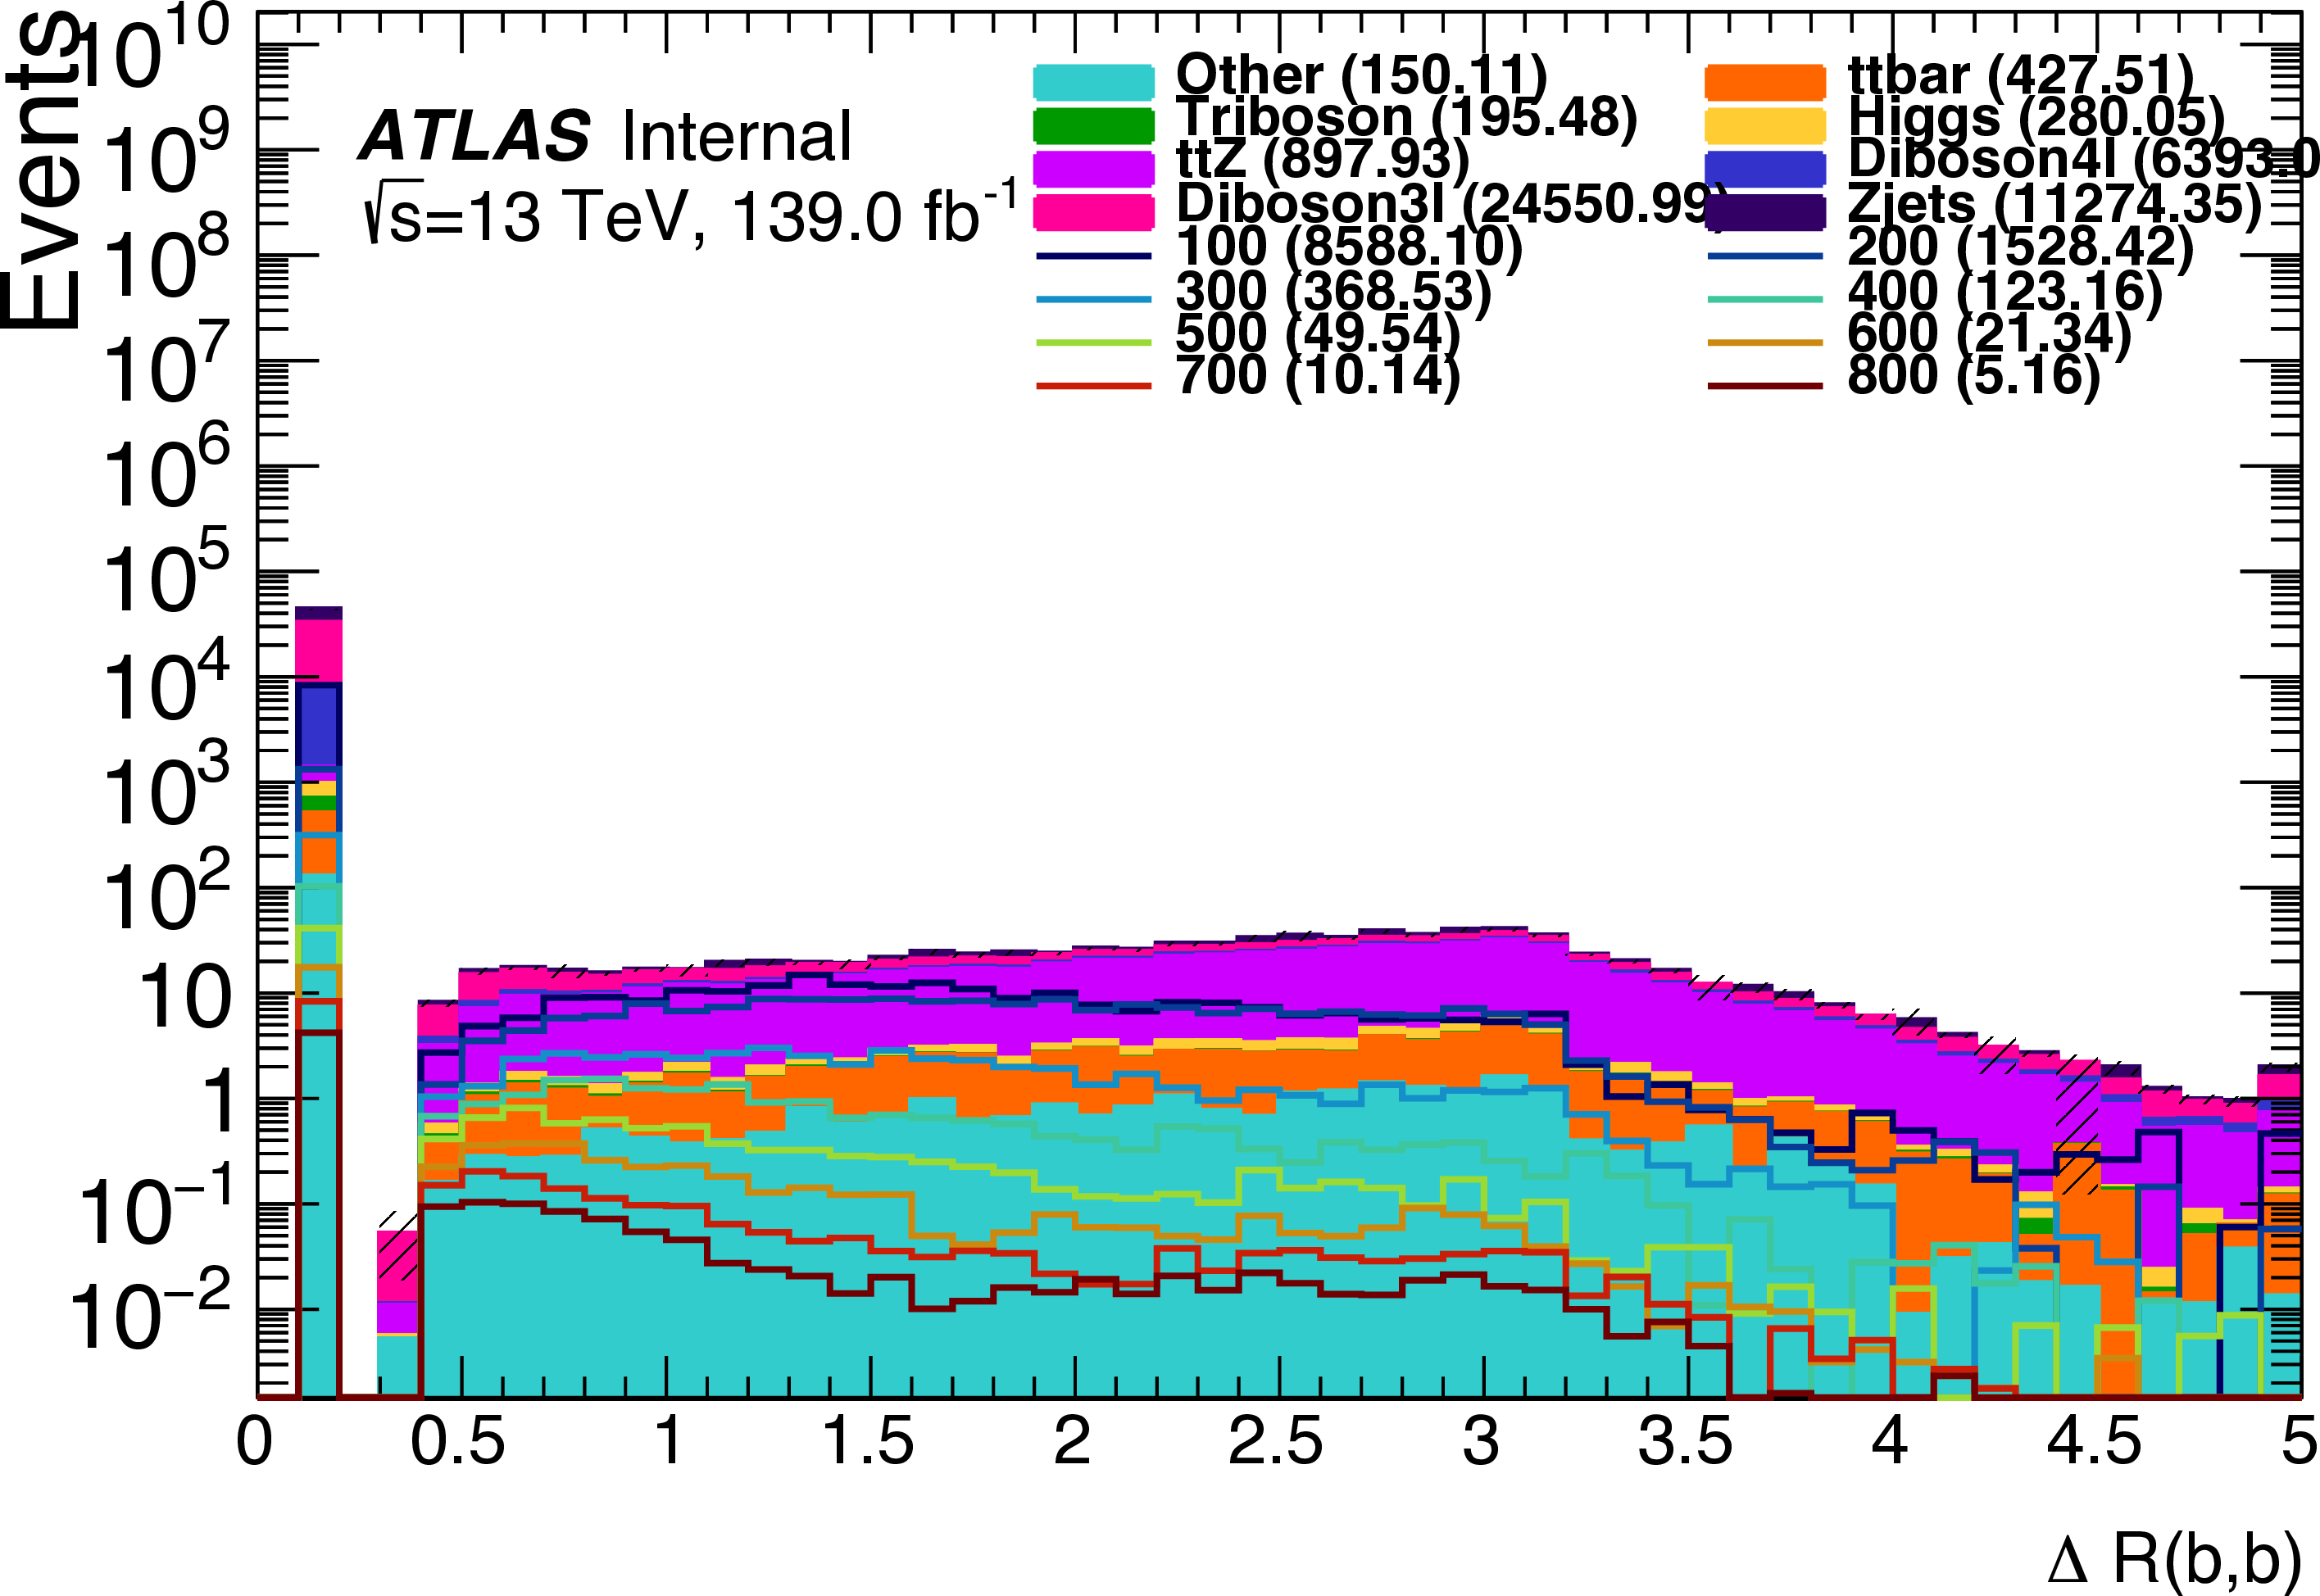
\includegraphics[width=0.98\textwidth]{figs/rpvthreel/dRbb_PreSel_logy_incl.png}
      \caption{}
      \label{fig:dRbb_PreSel_logy}
    \end{subfigure}
    \hfill
    \begin{subfigure}[b]{0.49\textwidth}
      \centering
      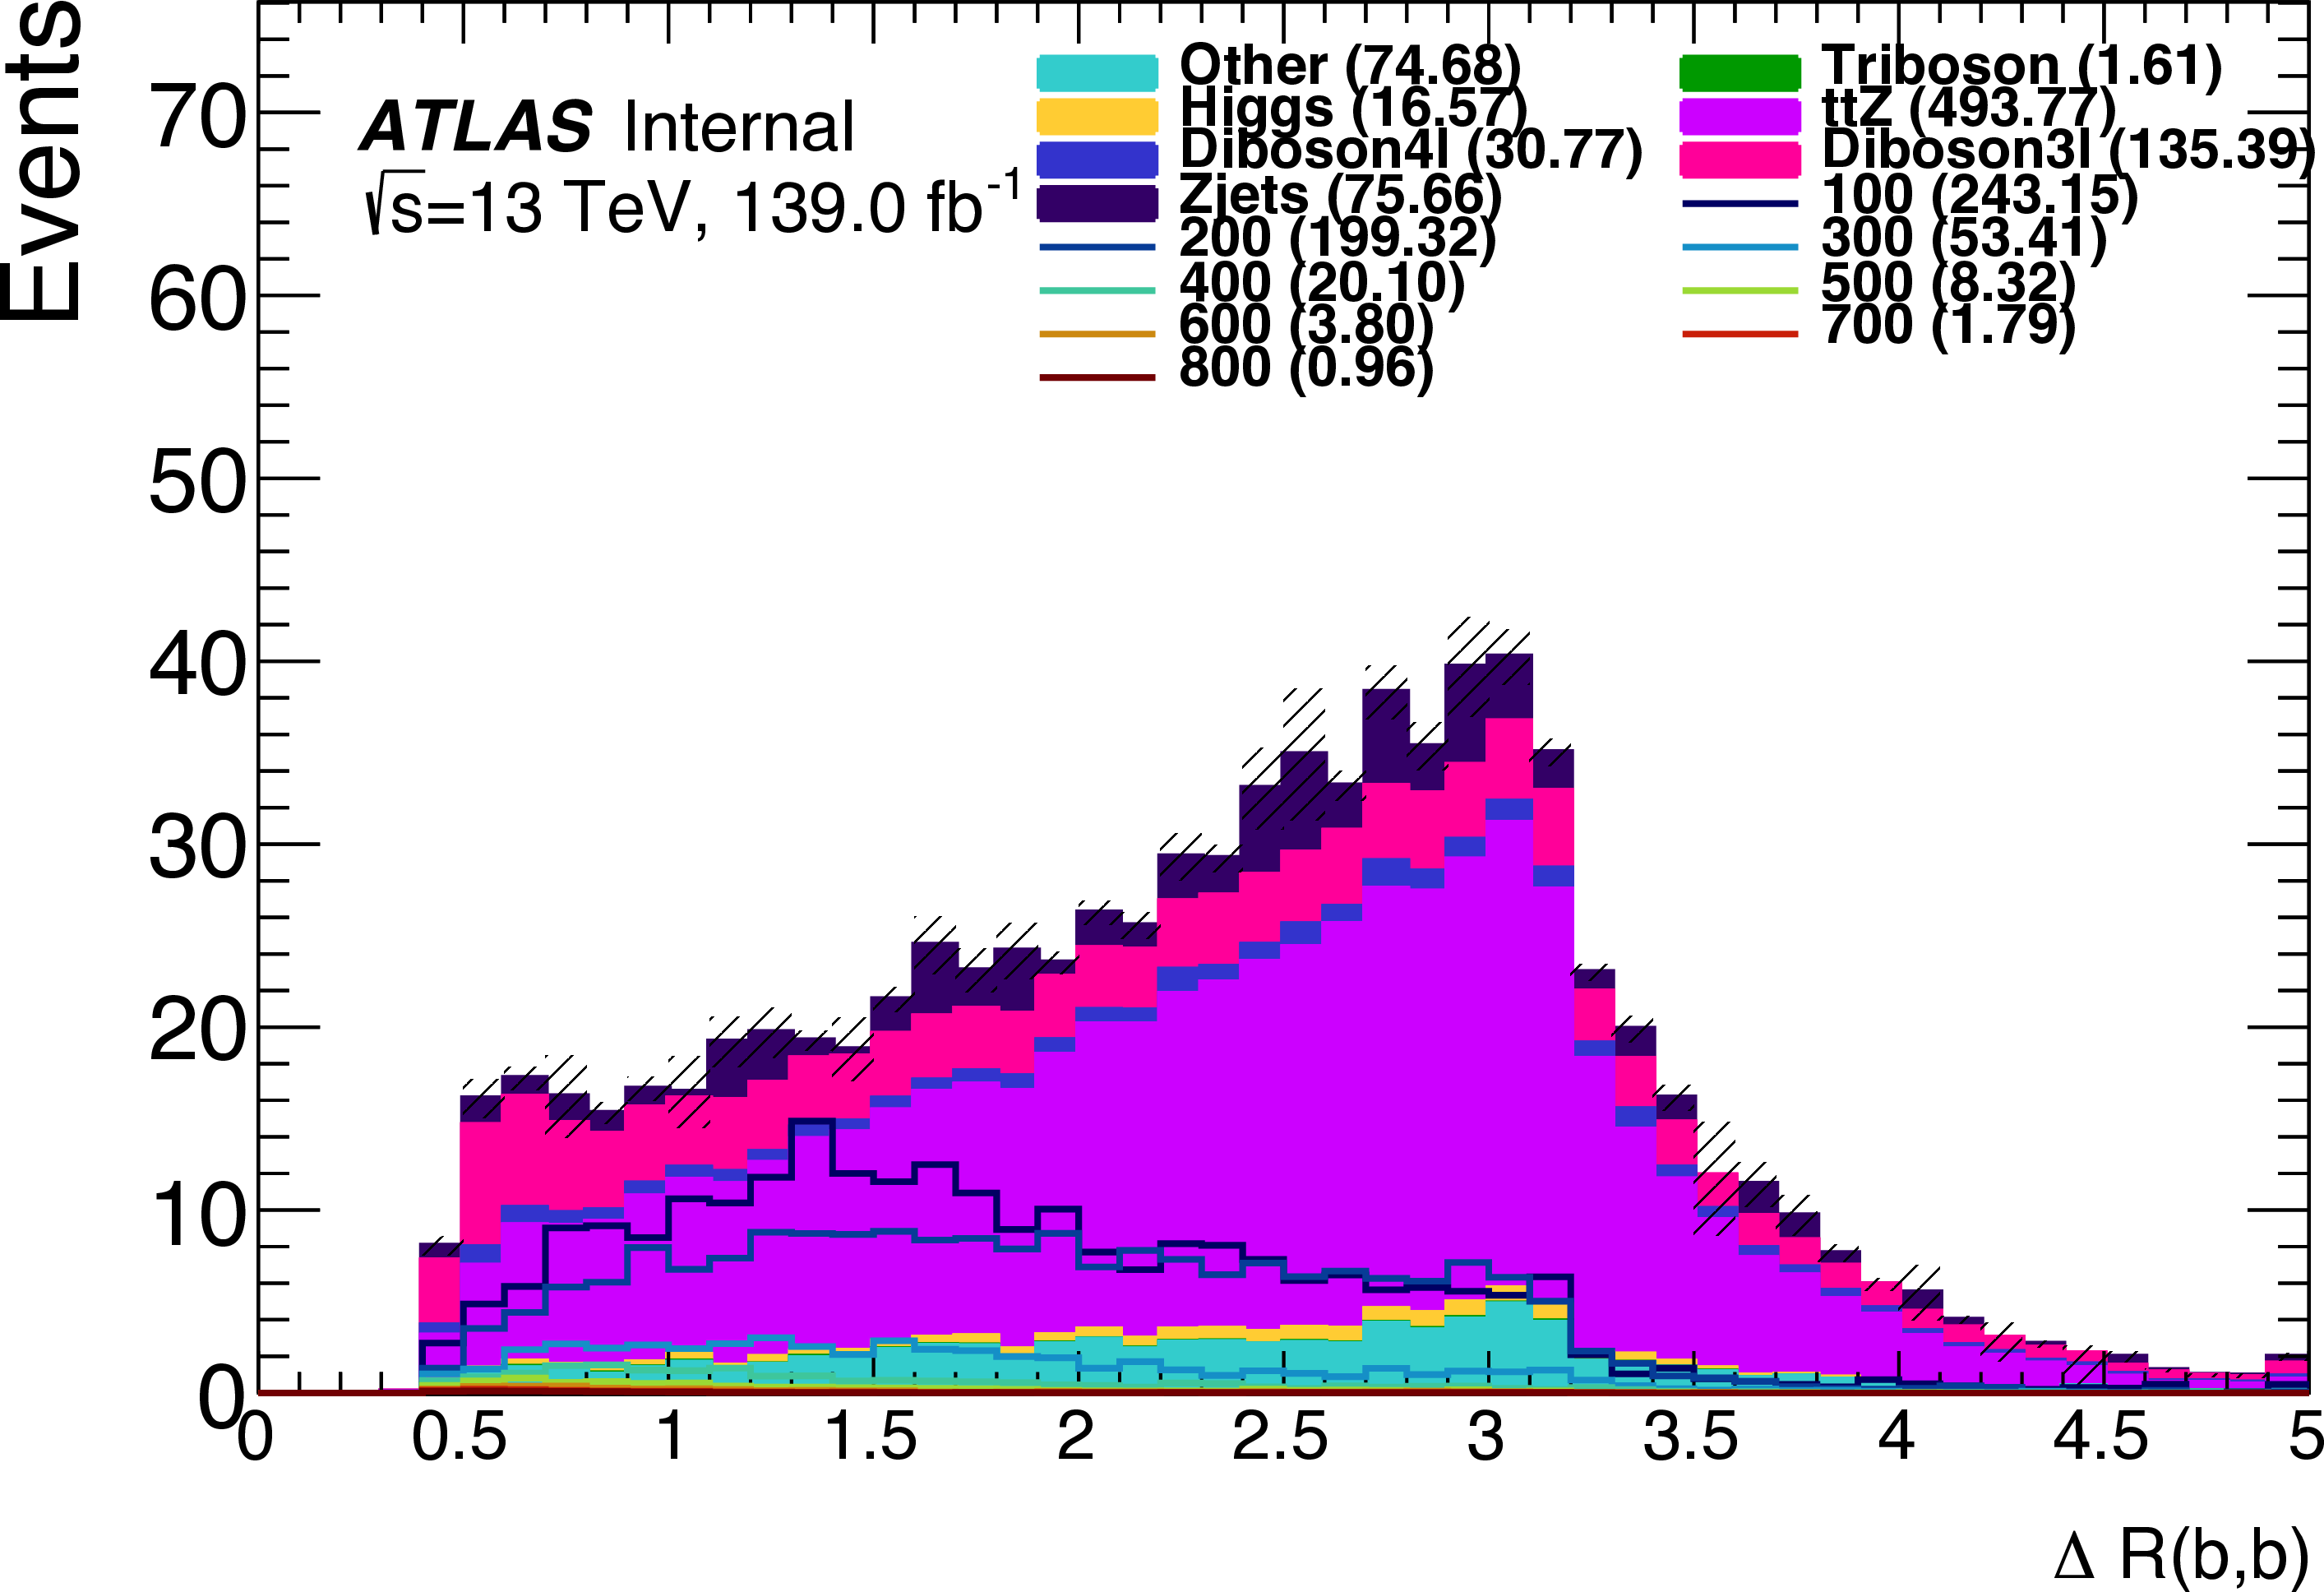
\includegraphics[width=0.98\textwidth]{figs/rpvthreel/dRbb_PreSel.png}
      \caption{}
      \label{fig:dRbb_Presel_lin}
    \end{subfigure}
  \caption{Expected distribution in simulation for background processes and signal processes of the angular separation between two $b$-tagged jets for events with three or more leptons (a) on a log scale where events without at least 2 $b$-jets have been assigned a value of 0.1, and (b) on a linear scale for events with at least 2 $b$-jets.}
          \label{fig:dRbb_PreSel}
\end{figure}
\begin{figure}[tbp]
    \centering
    \begin{subfigure}[b]{0.49\textwidth}
      \centering
      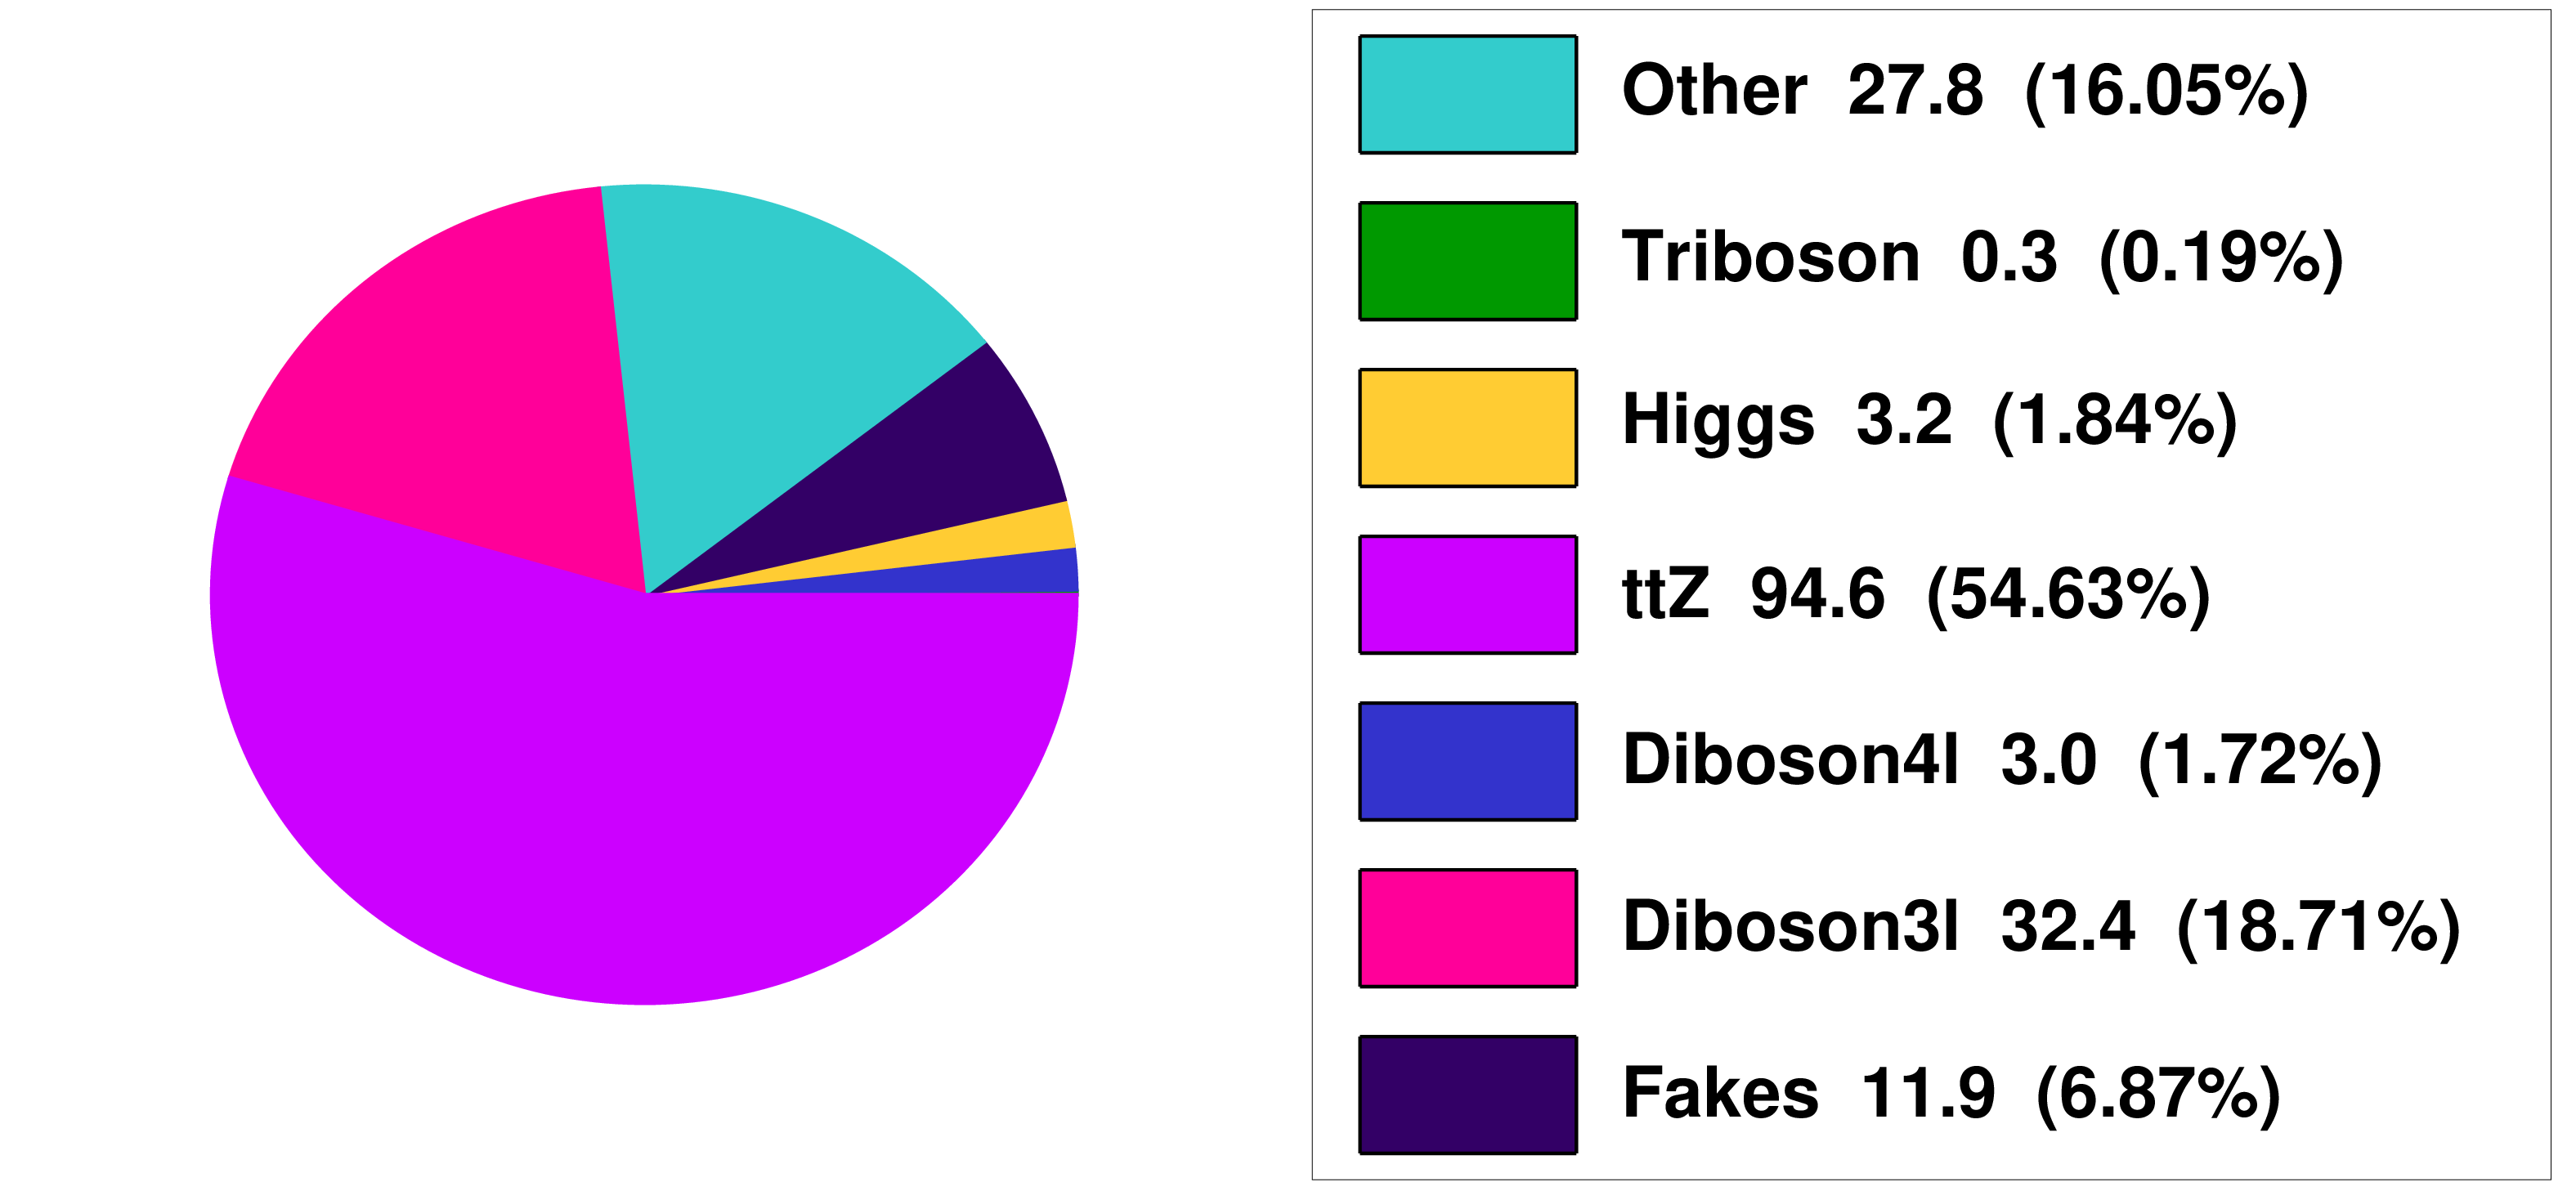
\includegraphics[width=0.98\textwidth]{figs/rpvthreel/CRttZ_yields.png}
      \caption{}
      \label{fig:CRttZ_yields}
    \end{subfigure}
    \hfill
    \begin{subfigure}[b]{0.49\textwidth}
      \centering
      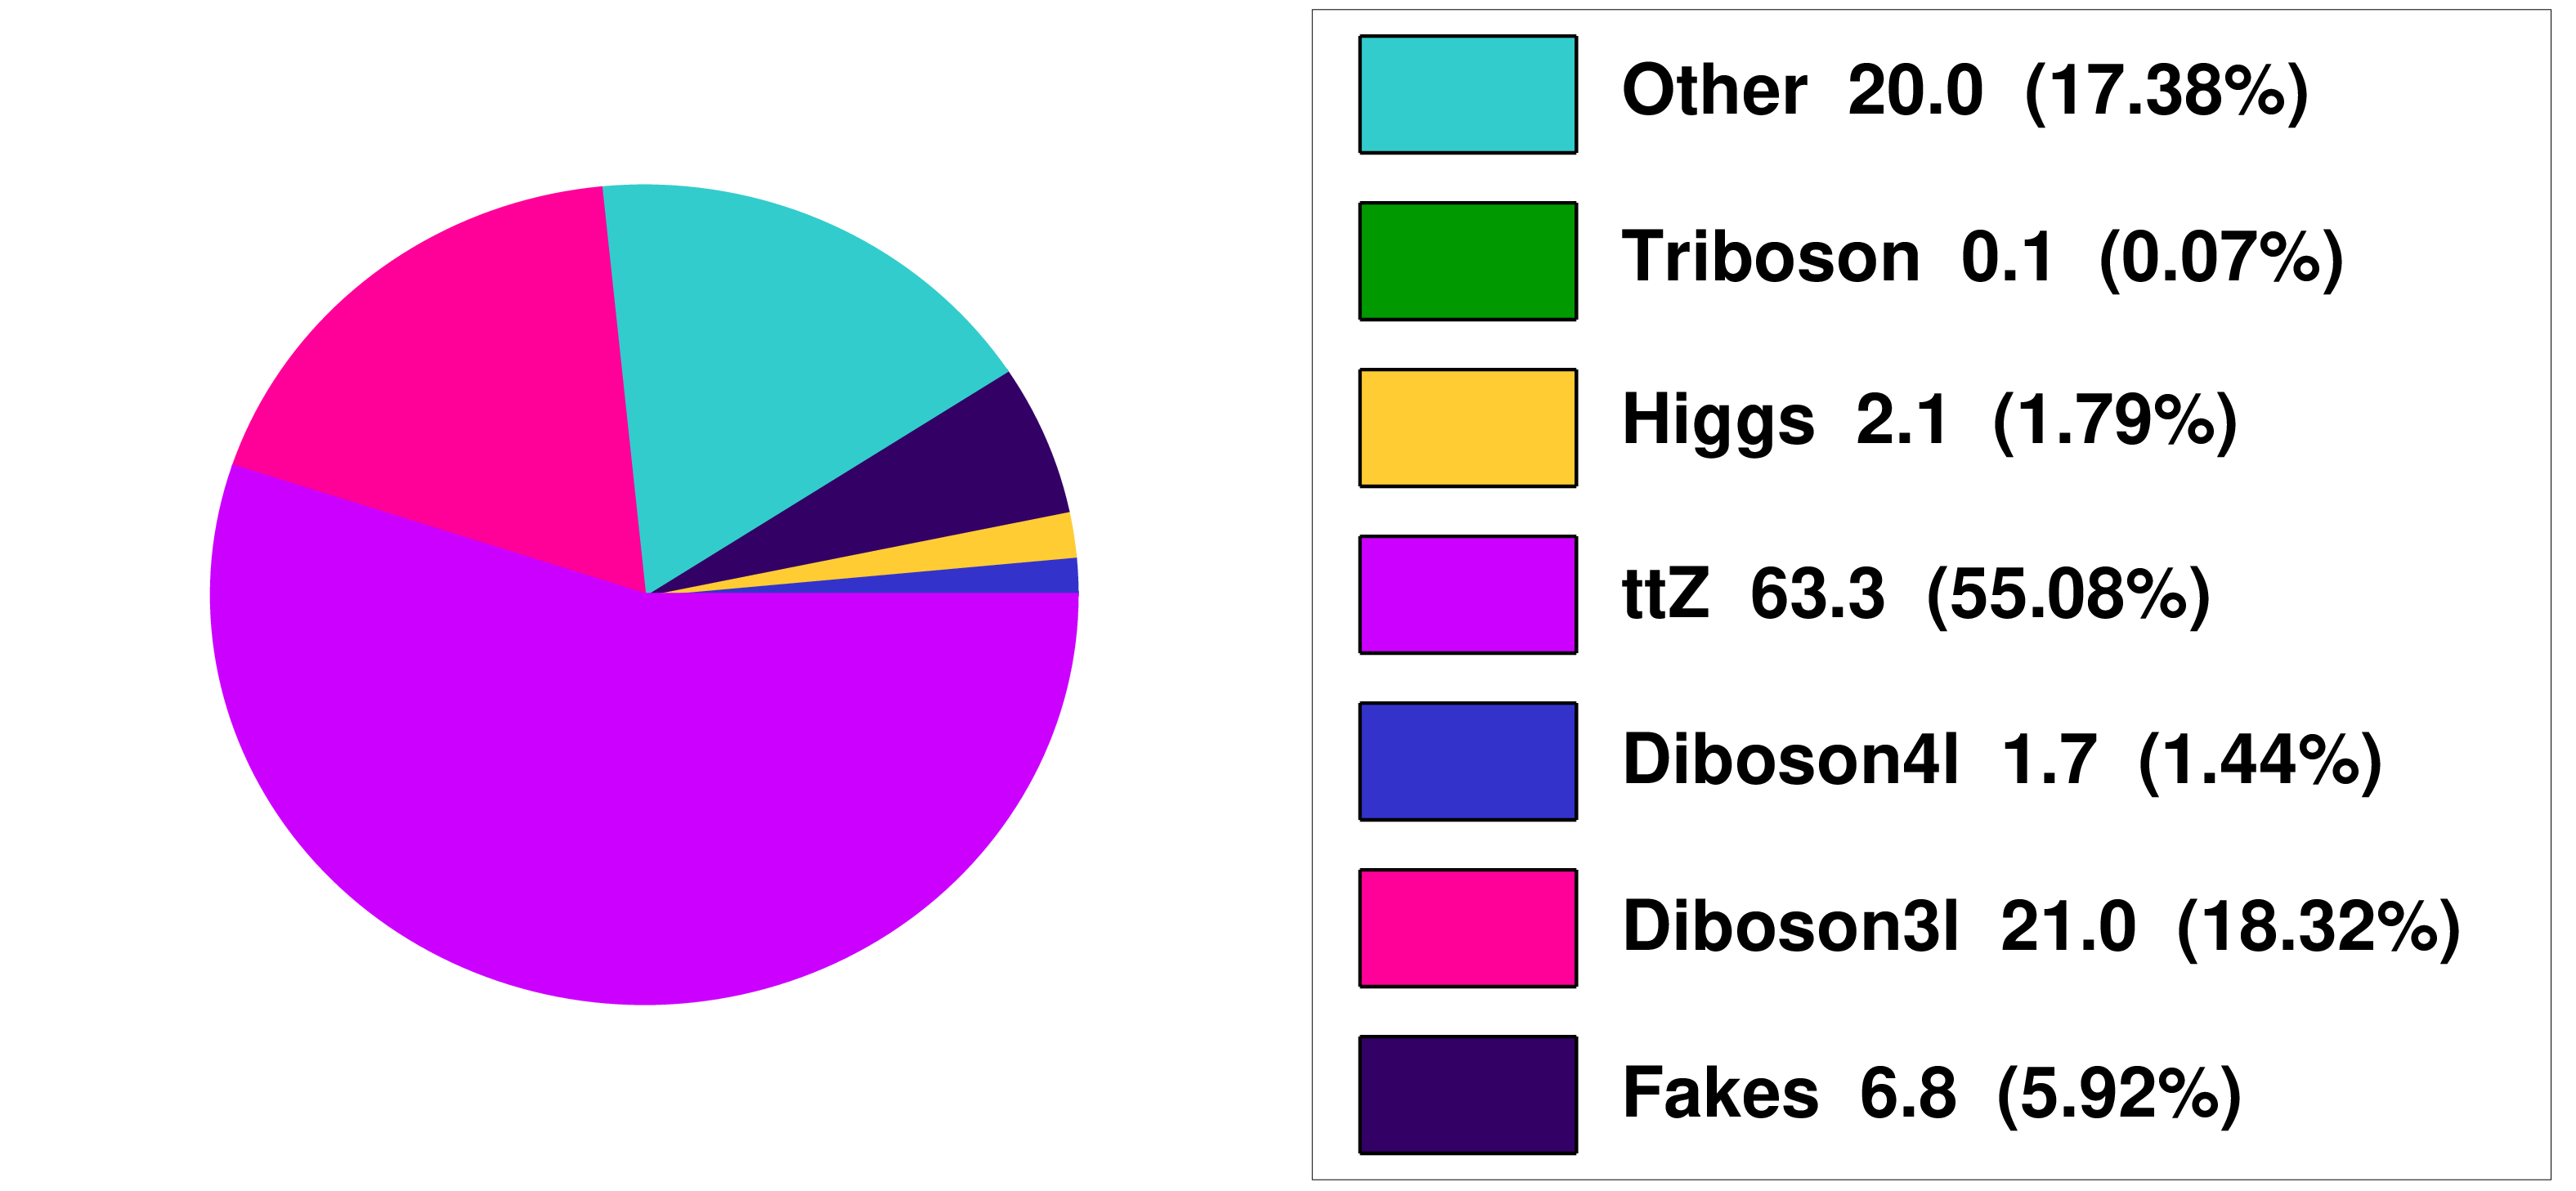
\includegraphics[width=0.98\textwidth]{figs/rpvthreel/VRttZ_yields.png}
      \caption{}
      \label{fig:VRttZ_yields}
    \end{subfigure}
  \caption[Expected yields of each background in \CRttZ and \VRttZ, assuming 140 \ifb. No normalization factors are applied.]
          {Expected yields of each background in \CRttZ and \VRttZ, assuming 140 \ifb. No normalization factors are applied.}
   \label{fig:ttZ_yields}
\end{figure}

\begin{table}[ht!]
  \small
  \begin{center}
  \begin{tabular}{l|cccccccc}
    \toprule
    \multirow{2}{*}{Region} & \multirow{2}{*}{$N_{\mathrm{lep}}$} & \multirow{2}{*}{$N_{\mathrm{b-jet}}$} & \multirow{2}{*}{$\Delta R(b,b)\dagger$} & \multirow{2}{*}{\met} & \multirow{2}{*}{\mTmin} & \multirow{2}{*}{Second} & \multirow{2}{*}{\FourlTwoZ;} & \multirow{2}{*}{\mZl} \\
        & & & & [GeV] & [GeV] & boson & $|m_{ll,2}-m_{Z}|$ [GeV] & asymmetry \\
    \midrule
        \SRThree       & 3 & - & $<$1.5 & $>$150 & $>$125   & - & - & - \\
        \CRWZ          & 3 & - & $<$1.5 & $<$80  & [50,100] & - & - & - \\
        \VRmet         & 3 & - & $<$1.5 & $>$80  & $<$100   & - & - & - \\
        \VRmTmin       & 3 & - & $<$1.5 & $<$80  & $>$125   & - & - & - \\
        %%VRZj          & ==3 & - & $<$1.5 & $<$80  & $<$50  & - & - & - \\
        \CRZj          & 3 & - & $<$1.5 & $<$30  & $<$30    & - & - & - \\
        \VRZj          & 3 & - & $<$1.5 & [30,80]& $<$30.   & - & - & - \\
    \midrule
        \CRttZ & $\geq$3 & $\geq$2 & $>$2.5      & $>$40 & - & - & veto; $<$20  & - \\
        \VRttZ & $\geq$3 & $\geq$2 & [1.5,2.5] & $>$40 & - & - &  veto; $<$20 & - \\
    \midrule
        \SRFour & $\geq$4 & -    & $<$1.5 & $>$80* & -    & No  & veto; $<$20 & - \\
        \SRFR          & $\geq$4 & -    & $<$1.5 & -    & -    & Yes & veto; $<$20 & $<$ 0.1 \\
        \CRZZ          & 4       & -    & $<$1.5 & -    & -    & -   & require; $<$5 & - \\
        \VRZZ          & 4       & -    & $<$1.5 & -    & -    & -   & require; [5,20] & - \\
    \bottomrule
  \end{tabular}
  \end{center}
  \caption[Kinematic selections for each region used in this analysis.]{Kinematic selections for each region used in this analysis. All regions require a SFOS pair of light leptons with an invariant mass between 81.2~\GeV and 101.2~\GeV and a third light lepton, the invariant mass of which (\mZl) must be at least 90~\GeV. The dagger ($\dagger$) indicates that this cut is only applied for events with at least 2 b-jets. The ``second boson'' requirement is shown to make the orthogonality between \SRFour and \SRFR explicit. This second boson is usually reconstructed from two jets, but it can also be reconstructed from two SFOS leptons, with an invariant mass requirement that changes depending on the objects used, as described in \ref{sec:srfr}. This is distinct from the \FourlTwoZ criterion which only applies to a leptonic Z. The asterisk (*) in the \SRFour \met\ cut indicates that this cut is only applied for events with two pairs of SF leptons. This condition is also referred to as \MetSF.}
  \label{tab:regions:regionBreakdown}
\end{table}



